%% +++++++++++++++++++++++++++++++++++++++++ %%
%                                             %
%                  Mainfile                   %
%                                             %
%% +++++++++++++++++++++++++++++++++++++++++ %%

% Latex-Vorlage für Abschlussarbeiten am Institut für Fahrzeugsystemtechnik (FAST), Teilinstitut Fahrzeugtechnik am Karlsruher Institut für Technologie (KIT)

% Stand: 07.07.2017, Timo von Wysocki

% Vollständig überarbeitete Version der Abschlussarbeitsvorlagen von Timo Rohrberg (2009) und Dominique Labonte (2012)

% In der Finalen Version der Abschlussarbeit, ist die draft-Option in der Dokumentenklasse (\documentclass[draft]{scrbook}) auszukommentieren und die disable-option im todo-Paket (\usepackage[%disable]{todonotes}) einzukommentieren!

\documentclass[				% Koma-Script
%draft,                     % Wird das einkommentiert, werden Bilder nur als Platzhalter eingefügt (schnellere PDF-Generierung zum schnelleren Testen)
a4paper,                    % Richtige Größe der Textfläche (A4)
pagesize=auto,              % Richtige Größe des Papiers
11pt,                       % Schriftgröße
oneside,                    % Einseitiger Druck
headsepline,                % Linie nach der Kopfzeile
DIV=12,                     % Wird benötigt, um den Bereich auf dem Blatt zu definieren, in dem sich der Text befindet. DIV = 12: Faktor für die Satzspiegelkonstruktion. Je größer der Wert, desto mehr Textfläche (Kleinere Ränder an den Seiten und oben und unten). Siehe scrguide, S. 36. Automatische, von der Schriftgröße Abhängige Berechnung durch DIV=calc
headinclude = true,         % Wenn die Kopfzeile in der Satzspiegelkonstruktion mitberücksichtigt werden soll, also zum Textbereich gezählt werden soll. Sinnvoll, wenn Kopfzeile mit viel Inhalt, bei eher leeren Kopfzeilen wirkt der obere Rand mit eingeschalteter Option zu leer. (siehe scrguide S.43)
footinclude = false,        % wie headinclude mit Fußzeile
%mpinclude = true,          % wie headinclude mit Randnotizen. Nur Sinnvoll, wenn man sehr viele Randnotizen hat
%BCOR = 20mm,               % Bindekorrektur
listof=totocnumbered,       % Gibt den Abbildungs- und Tabellen-Verzeichnissen einen (nummerierten) Eintrag im Inhaltsverzeichnis
listof=entryprefix,			% Abbildung und Tabelle wird im Verzeichnis vor die NUmmer geschrieben
index=totoc,				% Schreibt den Index ins Inhaltsverzeichnis
toc=bibliography,			% Schreibt die Bibliografie ins Inhaltsverzeichnis
parskip = half,             % Behandlung von Absätzen. Abstände zwischen den Absätzen, Einzug am Anfang der ersten Absatzzeile etc. Optionen siehe scrguide S.78
captions=tableheading       % Formatierung von Tabellenüberschriften als ÜBERschrift
]{scrbook}

% Referenz auf scr-guide: https://komascript.de/~mkohm/scrguide.pdf

\setcounter{secnumdepth}{2}	% Ebene, bis zu der nummeriert wird (chapter = 0; section = 1; etc.)
\setcounter{tocdepth}{5}	% Ebene bis zu der Überschriften im Inhaltsverzeichnis stehen (chapter = 0; section = 1; etc.)

%% +++++++++++++++++++++++++++++++++++++++++ %%
%                                             %
%               Standardklassen               %
%                                             %
%% +++++++++++++++++++++++++++++++++++++++++ %%

\usepackage[english]{babel}	% Sprache innerhalb des Dokuments (z.B. Überschrift toc)
\usepackage[T1]{fontenc}	% Lädt Zeichensatz mit Umlauten, nötig für korrekte deutsche Trennung
\usepackage[utf8]{inputenc}	% Umlaute können direkt eingetippt werden: äöüß
\usepackage{microtype}		% Ordentlicher Randausgleich 

\makeatletter
\renewcommand{\@pnumwidth}{3em}
\renewcommand{\@tocrmarg}{4em}
\makeatother
%\renewcommand\@pnumwidth{3em}% statt `2em' evtl. groesserer Wert 

\usepackage{blindtext}		% Fülltext zum Testen

\usepackage{tikz}			% Erstellen von Graphen
\usepackage{pgfplots}		% TEST IN PROGRESS
\pgfplotsset{compat=newest}
%\pgfdeclarelayer{bg}    % declare background layer
%\pgfsetlayers{bg,main}
\usepgfplotslibrary{groupplots}

\usepackage{filecontents}	% TEST IN PROGRESS

\usetikzlibrary{calc}		% Zusatzbibliothek für Tikz, um Berechnungen durchzuführen
\usetikzlibrary{arrows}
\usetikzlibrary{backgrounds}
\usetikzlibrary{chains}
\usetikzlibrary{circuits}
\usetikzlibrary{decorations.pathmorphing}
\usetikzlibrary{decorations.markings}
\usetikzlibrary{fadings}
\usetikzlibrary{fit}
\usetikzlibrary{intersections}
\usetikzlibrary{matrix}
\usetikzlibrary{positioning}
\usetikzlibrary{patterns}
\usetikzlibrary{scopes}
\usetikzlibrary{shadings}
\usetikzlibrary{shadows}
\usetikzlibrary{shapes}
\usepackage{url}

\usepackage{calc}			% Für berechnungen allgemein (genutzt bei Textboxen)

\usepackage[				% Textboxen absolut auf Seiten platzieren
absolute,					% Absolute Positionsangaben
overlay,					% Einfügen als Overlay über dem Text
]{textpos}
\usepackage{textfit}		% Text auf bestimmte Breite skalieren	

\usepackage{graphicx}		% Einbinden von Grafiken

\usepackage{pdfpages}		% Einbinden von PDF-Dateien

\usepackage{acronym}		% Für Abkürzungsverzeichnis

\usepackage{color,soul}			% Eigene Farben definieren

\usepackage{xcolor}

\usepackage{colortbl}

\usepackage[
%disable			% Diese Zeile aktivieren für finale Version! Deaktiviert alle Todos und Todoliste!
]{todonotes}      % Todos mit \todo{Aufgabe} als Randnotiz, kann als gesammelte Liste ausgegeben werden (Hier am Ende des Dokuments)

%% +++++++++++++++++++++++++++++++++++++++++ %%
%                                             %
%                  Kopfzeile                  %
%                                             %
%% +++++++++++++++++++++++++++++++++++++++++ %%

% Kein fancyhdr in Kombination mit KOMA!

% Siehe Coma-Anleitung, S.231


\usepackage[		% Das Koma-Script-Paket für Header und Footer
autooneside=false,	% Nötig, da einseitiger Druck
automark			% Definiert \leftmark und \rightmark sinnvoll
]{scrlayer-scrpage}

% Da das Dokument einseitig ist, ist jede Seite ungerade!

% Definition des Inhalts für die Kopfzeile
\lohead{\rightmark}			% lo = left odd, \rightrmark = Section, \leftmark = chapter
\cohead{}					% Mitte soll leer sein
\rohead{\pagemark}			% lo = right odd, \pagemark = Seitenzahl

% Mit diesen Einstellungen wird in der Kopfzeile solange das Kapitel angezeigt, bis die erste Section definiert wird. Ab da nur noch die sections.

\cofoot{}					% entfernt die Seitenzahl in der Fußzeile

% Entfernen der Seitenzahl auf Kapitelseiten, da es keinen Sinn macht, die Seitenzahl auf einer einzelnen Seite wo anders hinzuschreiben:
\renewcommand*{\chapterpagestyle}{empty}


%% +++++++++++++++++++++++++++++++++++++++++ %%
%                                             %
%                 Schriftart                  %
%                                             %
%% +++++++++++++++++++++++++++++++++++++++++ %%

% Laden der serifenlosen Schriftart Helvetica:
\usepackage[
scaled
]{helvet}	% scaled skaliert die Schriftart, da helvetica größer its als andere Schriften. Werden in einem dokument verschiedene Schriften verwendet (z.B. Serifen oder Kapitälchen) sollte Helvetica skaliert werden. Die Option scaled ohne Größenangabe skaliert automatisch auf eine Standardschriftgröße.

% Zuweisen der Serifenlosen Schrift als Standardschrift
\renewcommand\familydefault{\sfdefault}

% Zeeilenabstand ändern:
\usepackage[onehalfspacing]{setspace}
% onehalfspaceing schaltet auf 1,5-fachen Zeilenabstand

%% +++++++++++++++++++++++++++++++++++++++++ %%
%                                             %
%                  Tabellen                   %
%                                             %
%% +++++++++++++++++++++++++++++++++++++++++ %%

\usepackage{tabularx} 
\usepackage{booktabs}	% Für schöne Tabellenzwischenlinien
\usepackage{arydshln}	% Für gestrichelte Tebellenlinien, nach longtable einbinden!
\usepackage{longtable}	% Für mehrseitige Tabellen
\usepackage{multirow}

% Erstellen neuer Tabellenspaltentypen
\usepackage{array}		% Benötigt, um Text in Tabellenzeilen mit fester Breite auszurichten
\newcolumntype{C}[1]{>{\centering\arraybackslash}p{#1}} % zentrierte Spalten mit Breitenangabe 
\newcolumntype{R}[1]{>{\raggedleft\arraybackslash}p{#1}} % rechtsbündig mit Breitenangabe 

%% +++++++++++++++++++++++++++++++++++++++++ %%
%                                             %
%                  SI-Units                   %
%                                             %
%% +++++++++++++++++++++++++++++++++++++++++ %%

% Mit dem Paket werden Zahlen mit Einheiten mit einem halben geschützten Leerzeichen gesetzt, sowie Darstellungen können global geändert werden.

\usepackage[
per-mode=symbol,			% Darstellung von Einheitenbrüchen %[per-mode=symbol] oder [per-mode=fraction]. 1.Schrägstrich, 2. Bruchstrich
decimalsymbol=comma,		% Dezimalsymbol (Zahl immer mit Punkt schreiben!)
exponent-product = \cdot,	% Malzeichen für *10^n
repeatunits=false,			% Einheiten wiederholen bei SIrange
tophrase={{ bis }}	% benötigt 2 Klammern, wegen den Leerzeichen
]{siunitx}	% Darstellung von Zahlen mit Einheiten
\usepackage{siunitx}

% Eigene Einheiten definieren:
\DeclareSIUnit\g{g}	% Gewichtskraft
\DeclareSIUnit{\million}{\text{Mio.}}	% Million z.B. \million\kilo\metre
\DeclareSIUnit{\none}{-}	% Keine Einheit

% Benutzung:
% \SI{5}{\kilo\hertz} -> 5 kHz
% \si{\hertz} -> Hz
% \SIrange{5}{10}{\kilo\hertz} -> 5 bis 10 kHz

%% +++++++++++++++++++++++++++++++++++++++++ %%
%                                             %
%          Codedarstellung im Text            %
%                                             %
%% +++++++++++++++++++++++++++++++++++++++++ %%

% Farbdefinitionen
\definecolor{mycomment}{rgb}{0.4,0.4,0.4}
\definecolor{mykeyword}{rgb}{0,0,1}
\definecolor{mynumber}{rgb}{0.5,0.5,0.5}
\definecolor{mystring}{rgb}{0.58,0,0.82}

\usepackage{scrhack}			% Wird benötigt, damit ein Bug zwischen listings und koma-Script behoben wird
\usepackage{listings}			% Darstellung von Codebeispielen
\lstset{%
	language=Matlab,	 		%Standardsprache, wenn keine Option angegeben wird. Individuell änderbar mit \begin{lstlisting}[language=Python]...\end{lstlisting}. Auflistung verfügbarer Sprachen. https://en.wikibooks.org/wiki/LaTeX/Source_Code_Listings
	frame=single,				% Rahmen um den Code	
	extendedchars=true, 		% Für nicht Ascii-Zeichen, jedoch nur bei Latin-Codierung. UTF8 benötigt spezielle Definition unten
	basicstyle=\footnotesize,	% Schriftgröße des Codes
	basicstyle=\ttfamily,		% Schriftart des Codes als Monospace
	numbers=left,				% Zeilennummern links
	%tabsize=2,					% Breite für Tabs
	commentstyle=\color{mycomment},		% Farbe für Kommentare
	keywordstyle=\color{mykeyword}, 	% Farbe für Keywords
	numberstyle=\tiny\color{mynumber},	% Farbe für Zeilennummern
	stringstyle=\color{mystring},	% Farbe für Strings
	showspaces=false,			% Markiere Leerzeichen im Code
	showstringspaces=false,		% Markiere Leerzeichen in Strings
	breaklines=true,			% Aktiviert Zeilenumbrüche innerhalb des Codes (ansonsten laufen zu lange Zeilen nach rechts aus der Seite raus)
	breakatwhitespace=false,    % Sollen Zeilenumbrüche nur an Leerzeichen gestattet sein?	
	escapeinside={\%*}{*)},		% Escapecharacter um Latex-Code zwischen den Code zu schreiben. Verwendung: %*\label{codeline:add}*). Werden verschiedene Sprachen in einem Dokument definiert, kann es sinnvoller sein, die Escapecharacters individuell in den optionen der lstlisting-Umgebung zu definieren, so dass in jeder Sprache der Escapecharacter mit dem entsprechenden Kommentarsymbol beginnt.
}  

%\renewcommand{\lstlistingname}{Codebeispiel}	% Umbenennen der Code-Umgebung

% Behandlung von nicht Ascii-Zeichen in UTF8-Dokumenten
\lstset{literate=
	{á}{{\'a}}1 {é}{{\'e}}1 {í}{{\'i}}1 {ó}{{\'o}}1 {ú}{{\'u}}1
	{Á}{{\'A}}1 {É}{{\'E}}1 {Í}{{\'I}}1 {Ó}{{\'O}}1 {Ú}{{\'U}}1
	{à}{{\`a}}1 {è}{{\`e}}1 {ì}{{\`i}}1 {ò}{{\`o}}1 {ù}{{\`u}}1
	{À}{{\`A}}1 {È}{{\'E}}1 {Ì}{{\`I}}1 {Ò}{{\`O}}1 {Ù}{{\`U}}1
	{ä}{{\"a}}1 {ë}{{\"e}}1 {ï}{{\"i}}1 {ö}{{\"o}}1 {ü}{{\"u}}1
	{Ä}{{\"A}}1 {Ë}{{\"E}}1 {Ï}{{\"I}}1 {Ö}{{\"O}}1 {Ü}{{\"U}}1
	{â}{{\^a}}1 {ê}{{\^e}}1 {î}{{\^i}}1 {ô}{{\^o}}1 {û}{{\^u}}1
	{Â}{{\^A}}1 {Ê}{{\^E}}1 {Î}{{\^I}}1 {Ô}{{\^O}}1 {Û}{{\^U}}1
	{œ}{{\oe}}1 {Œ}{{\OE}}1 {æ}{{\ae}}1 {Æ}{{\AE}}1 {ß}{{\ss}}1
	{ű}{{\H{u}}}1 {Ű}{{\H{U}}}1 {ő}{{\H{o}}}1 {Ő}{{\H{O}}}1
	{ç}{{\c c}}1 {Ç}{{\c C}}1 {ø}{{\o}}1 {å}{{\r a}}1 {Å}{{\r A}}1
	{€}{{\euro}}1 {£}{{\pounds}}1 {«}{{\guillemotleft}}1
	{»}{{\guillemotright}}1 {ñ}{{\~n}}1 {Ñ}{{\~N}}1 {¿}{{?`}}1
}        

%% +++++++++++++++++++++++++++++++++++++++++ %%
%                                             %
%                    Mathe                    %
%                                             %
%% +++++++++++++++++++++++++++++++++++++++++ %%

\usepackage{amsmath}		% Mathe-Paket. Z.B. für \align
\usepackage{amssymb}		% Mathe-Symbole, lädt automatisch amsfonts mit, insbesondere Mengen
\usepackage{amsbsy}			% Fette Mathe-Buchstaben
\usepackage{mathtools}

\newcommand{\punkt}{\quad\text{.}}
\newcommand{\komma}{\quad\text{,}}

% Vektoren:
%\newcommand{\ve}[1]{\vec{#1}}						% Vektorpfeil
%\newcommand{\ve}[1]{\underline{#1}}				% Unterstrich
\newcommand{\ve}[1]{\boldsymbol{#1}}				% Fettdruck

% Matrizen:
%\newcommand{\ma}[1]{\underline{\underline{#1}}}	% Doppelter Unterstrich
\newcommand{\ma}[1]{\boldsymbol{#1}}				% Fettdruck

%% +++++++++++++++++++++++++++++++++++++++++ %%
%                                             %
%                  Zitieren                   %
%                                             %
%% +++++++++++++++++++++++++++++++++++++++++ %%

\usepackage{cite}

%\usepackage{csquotes}	% Erweitert die Zitiermöglichkeiten, wird von Biblatex benötigt, sonst Warnung


%\usepackage[
%backend=biber,			% Backend für die Bibliografieerzeugung. %Alternativ Bibtex
%style=alphabetic,		% Stil des Literaturverzeichnisses
%citestyle=alphabetic	% Stil der Zitation
%]{biblatex} 

% Einbinden der Literaturdatei:
%\bibliography{./quellen/quellen}	


%% +++++++++++++++++++++++++++++++++++++++++ %%
%                                             %
%                  Variablen                  %
%                                             %
%% +++++++++++++++++++++++++++++++++++++++++ %%

%% +++++++++++++++++++++++++++++++++++++++++ %%
%                                             %
%              Persönliche Daten              %
%                                             %
%% +++++++++++++++++++++++++++++++++++++++++ %%

% 07.07.2017 Timo von Wysocki

% Hier alles ausfüllen und bei Bedarf einkommentieren. Es muss nichts an den ersten vier Seiten von Hand geändert werden. Es kann alles hier in diesem Dokument eingestellt werden! Definiert den Inhalt für Titelseite, Aufgabenstellung sowie die Erklärungen zur Aufgabenstellung und Wissenschaftlichkeit.


\newcommand{\mydegree}{B.\,Sc.} % Akademischer Grad des Bearbeiters, \, = halbes geschütztes Leerzeichen
\newcommand{\anrede}{Mr}	% Herrn oder Frau oder leer
\newcommand{\myname}{Jinbo Chen}
\newcommand{\mymatnr}{1791575}
\newcommand{\mytitle}{Simulation of vehicle model for road features detection} % Titel der Arbeit
%\newcommand{\mysubtitle}{} % (Um zu benutzen nur einkommentiern, ausfüllen und compilen! Nichts im Deckblatt ändern)

% Adresse des Bearbeiters:
\newcommand{\mystreet}{Klosterweg.28}
\newcommand{\mytown}{76131 Karlsruhe, Germany}
\newcommand{\mytel}{49-176-7266-9331}

% Betreuer der Arbeit:
\newcommand{\reviewerone}{M.Sc. Johannes Masino}

% Um zu benutzen nur einkommentiern, ausfüllen und compilen! Nichts im Deckblatt ändern:
%\newcommand{\reviewertwo}{Name} 
%\newcommand{\advisor}{Name}
%\newcommand{\advisortwo}{Name}

\newcommand{\timestart}{01.08.17} 	% Startzeitpunkt
\newcommand{\timeend}{30.11.17}		% Endzeitpunkt
\newcommand{\datetitle}{Karlsruhe, November 2017}	% Das Datum, das auf der Titelseite steht
\newcommand{\dateerklaerung}{Karlsruhe, den 30.11.2017}	% Datum für die Erklärung zur Selbstständigkeit

% Pfad zum Titelbild:
\newcommand{\pathtitleimage}{./administration/grafiken/Titelbild.png} % Layout auf Titelbild im Format 1,618:1 optimiert
\newcommand{\numberthesis}{17-F-0114}	% Nummer der Arbeit
\newcommand{\thesistype}{Master Thesis}	% Typ der Arbeit

\newcommand{\projektleiter}{M.Sc. Johannes Masino} % Name des Projektleiters

% Hier kommt die Aufgabenstellung rein:
\newcommand{\aufgabenstellung}{%
%	Im Rahmen des industriegeförderten Forschungsprojektes sollen höhere Dimensionen erforscht werden.
%	Die Lösung der Aufgabenstellung erfolgt durch die Bearbeitung folgender Teilaufgaben:
The task of the research project is to detect the road features with data mining method in simulation environment.

The solution of this task is split into the following subtasks:
	\begin{itemize}
		\item Induction of the theme by researching about the current state of the art
		\item Implementation of different road surfaces and road damages.
		\item Further development of the full car model
		\item Extraciton of features for the Machine Learning.
		\item Training the Support-Vector Machine for the Machine Learning.
		\item Improving the classification for practical application
		\item Documentation of the entire work.
\end{itemize}
}

% Layouteinstellungen:

% Soll die Titelseite einen Rahmen besitzen?
\newif\ifFrame
\Frametrue
%\Framefalse

% Soll das Institutslogo oder die Institutsadresse angezeigt werden?
\newif\ifLogo
%\Logotrue
\Logofalse	


%% +++++++++++++++++++++++++++++++++++++++++ %%
%                                             %
%                    Index                    %
%                                             %
%% +++++++++++++++++++++++++++++++++++++++++ %%

\usepackage{makeidx}	% Paket zum Erstellen von Indizes
\makeindex				% Generiert den Index
% Index muss beim ersten mal von Hand erzeugt werden!


%% +++++++++++++++++++++++++++++++++++++++++ %%
%                                             %
%                  Hyperref                   %
%                                             %
%% +++++++++++++++++++++++++++++++++++++++++ %%

\usepackage[
bookmarksopenlevel=1,
bookmarksopen=true,		% öffnet die Bookmarks standardmäßig im adobe reader
bookmarksnumbered=true,
pdfborder={0 0 0.5},	% Setzt die Liniendicke von Kästen				
linkbordercolor={0 0.61 0.50},   
citebordercolor={0 0.61 0.50},
hyperfootnotes=false,	% Warum sollte man das abschalten?
linktoc=all				% Im Inhaltsverzeichnis ist Bezeichnung ond Seitenzahl ein Link
]{hyperref} 

\hypersetup{	% Titel etc. sollten erst nach dem laden des Pakets hyperref definiert werden
	pdfauthor={\myname},
	pdftitle={\mytitle},
	%pdfsubject={Not set},
	%pdfkeywords={Not set}
}


%% +++++++++++++++++++++++++++++++++++++++++ %%
%% +++++++++++++++++++++++++++++++++++++++++ %%
%                                             %
%                 MainDocument                %
%                                             %
%% +++++++++++++++++++++++++++++++++++++++++ %%
%% +++++++++++++++++++++++++++++++++++++++++ %%


\pgfplotsset{
	%xlabela/.style={Test test 123},
	default_figure/.style={
   scaled ticks=false,
   tick label style={/pgf/number format/fixed},
		every axis label/.append style={font=\footnotesize},
		legend style={font=\footnotesize, cells={anchor=west}, draw=none},
		title style={font=\footnotesize},
		tick label style={font=\footnotesize},
		every axis label/.append style={font=\footnotesize},
		every node near coord/.append style={font=\footnotesize},
		%unit markings=parenthesis, %all units inside (...)
		ylabel near ticks, xlabel near ticks, %remove white space
		%thick, %draw everything with thick lines
		separate axis lines, % important !
		unbounded coords=jump,
		scale only axis=true,
		%cycle list name=mycyclelist,
	},
%axis_2_figure/.style={default_figure,width=5cm,height=5cm},
%axis_1_middle_figure/.style={default_figure,width=5cm,height=5cm},
%axis_1_wide_figure/.style={default_figure,width=\linewidth,height=4cm},
%axis_1_big_figure/.style={default_figure,width=\linewidth,height=6.4cm},
	mygroupplot/.style={default_figure,	height=3cm, width=3.5cm},
   mygroupplotsmall/.style={default_figure,	height=1.5cm, width=3.5cm},
	mylineplot/.style={default_figure, height=3.5cm, width=0.7\linewidth},
compat=1.13,
  mlspectrogram/.style={
	default_figure,	height=3.5cm, width=3.5cm,
		enlargelimits=false, axis on top, use units,
    xlabel=Time (s),
    ylabel=Frequency (kHz),
    colormap={parula}{
            rgb255=(53,42,135)
            rgb255=(15,92,221)
            rgb255=(18,125,216)
            rgb255=(7,156,207)
            rgb255=(21,177,180)
            rgb255=(89,189,140)
            rgb255=(165,190,107)
            rgb255=(225,185,82)
            rgb255=(252,206,46)
            rgb255=(249,251,14)
        }, colorbar,
    colorbar style={ylabel=Power/Frequency (dB/Hz)},
  },
}

\newcommand{\myGroupSep}{50pt}
\newcommand{\myGroupVertSep}{60pt}
\newcommand{\myGroupVertSepWithout}{50pt}
\newcommand{\myLabelSep}{7ex}
\newcommand{\myLegendPosition}{(0.5,1.03)}


\definecolor{UniBlau}{cmyk}{1,0.7,0,0}
\definecolor{UniGruen}{cmyk}{0.6,0,1,0}
\definecolor{UniOrange}{cmyk}{0,0.3,1,0}
\definecolor{UniRot}{cmyk}{0.4,1,0,0}

\pgfplotscreateplotcyclelist{mycyclelist}{
{UniBlau, line width = 1pt},
{UniGruen, line width = 1pt},
{UniOrange, line width = 1pt},
{UniRot, line width = 1pt},
{UniBlau!50!UniGruen, line width = 1pt},
{UniGruen!50!UniOrange, line width = 1pt},
{UniOrange!50!UniRot, line width = 1pt},
{UniRot!50!UniBlau, line width = 1pt},
}

\begin{document}
	\frontmatter	% Schaltet u.a. in den römischen Nummerierungsmodus
	%% +++++++++++++++++++++++++++++++++++++++++ %%
%                                             %
%           Template für KIT-Rahmen           %
%                                             %
%% +++++++++++++++++++++++++++++++++++++++++ %%

% 07.07.2017 Timo von Wysocki

%% Erstellt den Ramen für die ersten vier Seiten inklusive Logos, Internetadressen und Anschriften. Zur Benutzung \titletemplate{Inhalt1}{Inhalt2}. Inhalt 1 wird korrekt in der Schriftfläche der Seite platziert. Inhalt 2 kann eigene Platzierungen oder Modifikationen enthalten.

% Abstände definieren:
\newcommand{\diameter}{25pt}		% Durchmesser des Bogens des Rahmens
\newcommand{\border}{19mm}			% Abstand des Rahmens zum Rand in mm
\newcommand{\logoborder}{7mm}		% Abstand des Logos zum Rand in mm
\newcommand{\titleBorder}{60mm} 	% Abstand des Textes zum Rand nach oben in mm
\newcommand{\imageBorder}{133mm}	% Abstand des Bildes zum Rand nach oben in mm
\newcommand{\reviewerBorder}{45mm}	% Abstand des Projektleiters zum Rand nach unten in mm
\newcommand{\webBorder}{5mm}		% Abstand der Website zum unteren Rand nach oben in mm

% Berechnen der Länge des Institutsnamens um Box zu erzeugen mit exakt dieser Breite um rechts ausgerichteten linksbündigen Text zu produzieren
\newlength{\institutsname}
\settowidth{\institutsname}{Institute of Vehicle Systems Technology} % Berechne die Breite diess Textes, für die ordentliche Ausrichtung des Adressblocks

% Neues Kommando mit 2 Inputparametern. Der erste wird in eine fertige Box geschrieben und platziert, im zweiten können beliebige Kommandos eingefügt werden, auch neue Boxen etc.
\newcommand{\titletemplate}[2]{
\begin{titlepage}	% Definiere eine Titlepage
	
% KIT-Rahmen um die Titlepage
\ifFrame
	\definecolor{FrameColor}{rgb}{0.5,0.5,0.5}
\else
	\definecolor{FrameColor}{rgb}{1,1,1}
\fi	

\begin{tikzpicture}[remember picture, overlay]
	\draw [color=FrameColor] 
	($(current page.north west)+(\border,-\border)$) -- % gerade linie von oben links 
	($(current page.north east)+(-\border-\diameter, -\border)$) % nach oben recht bis vor den Bogen
	arc (90:0:\diameter) -- % Bogen
	($(current page.south east)+(-\border, \border)$) % Linie nach unten rechts
	-- ($(current page.south west)+(\border+\diameter,\border)$) % Linie nach unten Link bis vor den Bogen
	arc (90:0:-\diameter) -- % Bogen unten links
	cycle;	% schließe den Bogen	
	\end{tikzpicture}

	
	


% KIT-Logo:
\begin{textblock*}{10cm}(\border+ \logoborder ,\border+\logoborder)
	
\includegraphics[width=3.8cm]{./administration/grafiken/KIT.pdf}
\end{textblock*}
	
\ifLogo	
% Institutslogo:
\begin{textblock*}{10cm}[1,0](\paperwidth-\border-\logoborder,\border+\logoborder)
	\raggedleft
	
\includegraphics[width=4.8cm]{./administration/grafiken/institut_fast.png}
\end{textblock*}
\else
% Institutsadresse	
\begin{textblock*}{\institutsname}	[1,0](\paperwidth-\border-\logoborder,\border+\logoborder) % Ausrichten an Ecke rechts (1) oben (0) der Box	
		\small{\textbf{Institute of Vehicle Systems Technology}}\\
		\small{\textbf{Devision of Vehicle Technology}}\\
		\footnotesize{Head: Prof. Dr. rer. nat. Frank Gauterin}\\
		\footnotesize{Rintheimer Querallee 2}\\
		\footnotesize{76131 Karlsruhe}
\end{textblock*}	
\fi

% Userinput #1:
\begin{textblock*}{\textwidth}[0.5,0](\paperwidth/2,\titleBorder)
#1
\end{textblock*}

% Userinput #2:
#2

% KIT-Schriftzug unter Rahmen:
\ifFrame
\begin{textblock*}{10cm}[0,0.5](\border+\logoborder,\paperheight-\border+\webBorder)
\tiny{ 
	\iflanguage{english}
		{KIT -- The Research University in the Helmholtz Association}
		{KIT -- Die Forschungsuniversität in der Helmholtz-Gemeinschaft}
}
\end{textblock*}
\fi

% KIT-WEbsite unter Rahmen
\ifFrame
\begin{textblock*}{5cm}[1,0.5](\paperwidth-\border-\logoborder,\paperheight-\border+\webBorder)
	\raggedleft
	% Versuche, den Link klickbar zu machen, ohne optischen Rahmen
	%\hypersetup{hidelinks=true}
	%\href{www.kit.edu}{\large{	\textbf{www.kit.edu}}}
	%\hypersetup{hidelinks=false}
	\large{	\textbf{www.kit.edu}}	
\end{textblock*}
\fi

\end{titlepage}}
	
	%% +++++++++++++++++++++++++++++++++++++++++ %%
%                                             %
%                   Deckblatt                 %
%                                             %
%% +++++++++++++++++++++++++++++++++++++++++ %%

% 07.07.2017 Timo von Wysocki

%% Beinhaltet Seite 1 der offiziellen Anfangsseiten mit dem Deckblatt. Der Inhalt wird in der Datei ./inhalt/0000_persoenliche_daten definiert!


\titletemplate{	% 1. Input für titletemplate:
	\centering
	\textbf{\scaletowidth{8cm}{\thesistype}} % Die Leerzeilen sind wichtig!
	
	\vspace{0.5cm}
	\huge{\mytitle}
	
	\ifx\mysubtitle\undefined
	\else
	\vspace{0.5cm}		
	\Large{\textit{\mysubtitle}}
	\fi
	
	\vspace{0.5cm}
	\Large{\mydegree{} \myname}	
	
}{

% Titelbild
\begin{textblock*}{\textwidth}[0.5,0](\paperwidth/2,\imageBorder)
	\centering
	\vspace{3cm}
	\includegraphics[width=0.7\paperwidth]{\pathtitleimage}
\end{textblock*}	

\begin{textblock*}{\textwidth}[0,1](\border+\logoborder,\paperheight-\reviewerBorder)
	\begin{tabular}{@{}lcl@{}}
	\iflanguage{english}{Reviewer}{Project Manager}: & \qquad  & \reviewerone\\
	% Füge weitere Namen ein, wenn diese definiert sind:
	\ifx\reviewertwo\undefined
	\else & \qquad  & \reviewertwo\\
	\fi
	\ifx\advisor\undefined
	\else & \qquad  & \advisor\\
	\fi
	\ifx\advisortwo\undefined
	\else & \qquad  & \advisortwo\\
	\fi
	\end{tabular}	
\end{textblock*}

% Nummer der Arbeit
\begin{textblock*}{4cm}[0,1](\border+\logoborder,\paperheight-\border-\logoborder)
	Nr.: \numberthesis
\end{textblock*}

\begin{textblock*}{5cm}[1,1](\paperwidth-\border-\logoborder,\paperheight-\border-\logoborder)
	\raggedleft
	\datetitle
\end{textblock*}}
	%% +++++++++++++++++++++++++++++++++++++++++ %%
%                                             %
%               Aufgabenstellung              %
%                                             %
%% +++++++++++++++++++++++++++++++++++++++++ %%

% 07.07.2017 Timo von Wysocki

%% Beinhaltet Seite 2 der offiziellen Anfangsseiten mit der Aufgabenstellung. Der Inhalt wird in der Datei ./inhalt/0000_persoenliche_daten definiert!

\titletemplate{		
	\begin{center}
		%\Huge{\thesistype}
		\Huge{Master Thesis}
		\vspace{0.2cm}
		
		%\large{für}\\
		\LARGE{\anrede{} \mydegree{} \myname}\\
		\vspace{0.2cm}
		
		\large{(Std.-Nr.: \mymatnr)}\\
		\vspace{0.5cm}
		
		\huge{\mytitle}\\
		\vspace{1cm}

		\huge{Scope of the Thesis}		
		
	\end{center}


\aufgabenstellung
}{}

	%% +++++++++++++++++++++++++++++++++++++++++ %%
%                                             %
%     Vollständigkeit der Aufgabenstellung    %
%                                             %
%% +++++++++++++++++++++++++++++++++++++++++ %%

% 07.07.2017 Timo von Wysocki

%% Beinhaltet Seite 3 der offiziellen Anfangsseiten mit der Erklärung zur Vollständigkeit der Aufgabenstellung. Der Inhalt wird in der Datei ./inhalt/0000_persoenliche_daten definiert!

\titletemplate{		
Hiermit wird die Vollständigkeit der Aufgabenstellung bestätigt. Alle darüber hinaus gehenden Aufgaben sind nicht Teil der Abschlussarbeit oder werden in der Ausarbeitung als solche kenntlich gemacht. Sollte es der/dem Studierenden, ohne eigenes Verschulden, nicht möglich sein, diese Aufgabenstellung in der vorgesehenen Bearbeitungszeit vollständig zu erfüllen, ist dies in der Ausarbeitung zu begründen.
Mit ihrer/seiner Unterschrift nimmt die/der Studierende  die Aufgabenstellung an. 
Der Ausgabe- sowie Abgabetag ist somit bindend
	
%Die Diplomarbeit ist im engen Kontakt mit dem Institut auszuarbeiten und bleibt dessen Eigentum. Eine Einsichtnahme Dritter darf nur nach Rücksprache mit dem Institut erfolgen.

\vspace{2cm}

\centering
\begin{tabular}{@{}p{0.4\textwidth}p{0.1\textwidth}p{0.4\textwidth}@{}}
	Ausgabetag: \timestart &&Abgabetag: \timeend\\
	&&\\
	Betreuer:&&Projektleiter:\\
	&&\\
	&&\\
	&&\\	\cdashline{1-1}\cdashline{3-3}
	(Prof. Dr.rer.nat. Frank Gauterin)&&(\projektleiter)\\
	&&\\
	&&\\
	&&\\
	Bearbeiter:&&Anschrift:\\
	&&\\
	&& \mystreet\\
	&& \mytown\\ \cdashline{1-1}
	(\mydegree{} \myname)&&Tel.: \mytel\\
\end{tabular}

}{}

	%% +++++++++++++++++++++++++++++++++++++++++ %%
%                                             %
%        Erklärung zur Selbstständigkeit      %
%                                             %
%% +++++++++++++++++++++++++++++++++++++++++ %%

% 07.07.2017 Timo von Wysocki

%% Beinhaltet Seite 4 der offiziellen Anfangsseiten mit der Erklärung zur Selbstständigkeit und wissenschaftlichen Praxis. Der Inhalt wird in der Datei ./inhalt/0000_persoenliche_daten definiert!


\titletemplate{
\textbf{\Large Erklärung zur Selbstständigkeit und wissenschaftlichen Praxis}

Hiermit versichere ich, die Arbeit selbstständig verfasst und keine anderen als die angegebenen Quellen und Hilfsmittel benutzt sowie, die wörtlich oder inhaltlich übernommenen Stellen als solche kenntlich gemacht zu haben.

Die Satzung des Karlsruher Instituts für Technologie (KIT) zur Sicherung guter wissenschaftlicher Praxis in der jeweils gültigen Fassung habe ich beachtet.

\begin{tabular}{@{}p{0.4\textwidth}@{}}
	\\
	\\
	\\ \cdashline{1-1}
	\footnotesize \dateerklaerung
\end{tabular}
}{}

	
	
	%% +++++++++++++++++++++++++++++++++++++++++ %%
%                                             %
%            Kurzfassung der Arbeit           %
%                                             %
%% +++++++++++++++++++++++++++++++++++++++++ %%

%% Seite 5 der Arbeit

\addchap{Kurzfassung}
\thispagestyle{empty}
\section*{Simulation des Fahrzeugmodells zur Erkennung von Straßenmerkmalen}

% Hier Text einfügen:

Der Zustand der Straßeninfrastruktur beeinflusst Wohlstand, Produktivität, Wachstum und soziales Wohlergehen moderner Volkswirtschaften.
%
Die gegenwärtige Praxis der Straßenzustandsüberwachung ist mühsam und zeitaufwendig, da die meisten Schritte des Prozesses manuell durchgeführt werden.
%
Nur wenige Länder verfügen über die teure Spezialfahrzeuge für eine automatisierte Datenerhebung.
%
Außerdem die Überwachung ist nur in festen Intervallen von 1 bis 4 Jahren stattgefunden.
%
Mit der gegenwärtigen Praxis ist es unmöglich, dass Defekte in die frühe Phase umfassend identifiziert werden, bis die Reparaturen kosteneffizienter sind.
%
Vision-basierte Systeme können nur dann sehr umfassende Informationen liefern, wenn die Sichtlinie nicht behindert wird und genügend Rechenressourcen verfügbar sind.
%
Daher wurden neue Verfahren auf der Basis von Fahrzeugsensoren, insbesondere ein Inertialsensor, in der Fahrzeugkarosserie und überwachtes maschinelles Lernen entwickelt, um die Straßeninfrastruktur automatisch zu überwachen.
%
Überwachte maschinelle Lerntechniken beinhalten jedoch eine kostspielige und mühsame Sammlung von gelabelten Daten zum Trainieren und Testen.
%
Wir haben eine neuartige Simulationsumgebung entwickelt, um diese Kosten zu reduzieren und spezifische Fahrzeugparameter und Einstellungen für die Klassifikationsergebnisse zu untersuchen und zu quantifizieren.
%
Die entwickelten Simulationen und Ergebnisse ist hilflich für die Verbesserung von dem Modell um den realen Anwendungen.
	%% +++++++++++++++++++++++++++++++++++++++++ %%
%                                             %
%             Abstract  der Arbeit            %
%                                             %
%% +++++++++++++++++++++++++++++++++++++++++ %%

%% Seite 6 der Arbeit

\addchap{Abstract}
\thispagestyle{empty}
\section*{Simulation of vehicle model for road features detection}

% Hier Text einfügen:
% \blindtext

The condition of the road infrastructure influences the prosperity, productivity, growth and social wellbeing of modern economies.
%
Current practice of road condition monitoring is laborious and time-consuming as most steps of the process are done manually.
%
Few countries have expensive specialized vehicles for an automated data collection whereas the monitoring is only scheduled in fixed intervals of 1 to 4 years.
%
With current practice defects are unlikely to be comprehensively identified in early stages, when repairs are more cost-efficient.
%
Vision-based systems can provide very comprehensive information only when the line of sight is not obstructed and enough computational resources are available.
%
Therefore, new methods based on vehicle sensors, especially an inertial sensor, in the vehicle body, and supervised machine learning have been developed to autonomously monitor the road infrastructure.
%
However, supervised machine learning techniques involve a costly and laboriously collection of labeled data for training and testing.
%
We have developed a novel simulation environment to reduce these costs and to investigate and quantify specific vehicle parameters and settings on the classification results.
%
The developed simulation and results help to improve the models for real world applications.

	%% +++++++++++++++++++++++++++++++++++++++++ %%
%                                             %
%                  Danksagung                 %
%                                             %
%% +++++++++++++++++++++++++++++++++++++++++ %%

%% Seite 7 der Arbeit

\addchap{Danksagung}
\thispagestyle{empty}

% Hier Text einfügen:

An dieser Stelle möchte ich mich bei all denjenigen bedanken, die mich während der Anfertigung dieser Masterarbeit unterstützt und motiviert haben.

Zuerst gebührt mein Dank Herr Johannes Masino, der meine Masterarbeit betreut und begutachtet hat und mir mit viel Geduld, Interesse und Hilfsbereitschaft zur Seite standen.
%
Für die hilfreichen Anregungen, die konstruktive Kritik bei der Erstellung dieser Arbeit möchte ich mich herzlich bei ihm bedanken, ohne die diese Arbeit nicht hätte entstehen können.

Ebenfalls möchte ich mich bei Herrn Prof. Frank Gauterin und Herrn Dr. Michael Frey bedanken, die mich mit allen seinen Mitteln unterstützten und ohne dessen Hilfe und Bemühungen diese Arbeit nicht zustande gekommen wäre.

Meinen Freunden Oliver, Zhe Pang und meiner Freundin Hui Wang danke ich besonders für den Hilfen und starken emotionalen Rückhalt über die Dauer meines gesamten Studiums.

Abschließend möchte ich mich bei meinen Eltern bedanken, die mir mein Studium durch ihre Unterstützung ermöglicht haben und stets ein offenes Ohr für meine Sorgen hatten.


Jinbo Chen,

Karlsruhe, 26.11.2017





	
	
	
	\microtypesetup{protrusion=false}	% Ordnet die Seitenzahlen ordentlicher an
	\tableofcontents	% Inhaltsverzeichnis	
	\microtypesetup{protrusion=true}
	
%	%% +++++++++++++++++++++++++++++++++++++++++ %%
%                                             %
%               Symbolverzeichnis             %
%                                             %
%% +++++++++++++++++++++++++++++++++++++++++ %%

\chapter{Symbolverzeichnis}

% Unterverzeichnisse (z.B. für lateinische und griechische Buchstaben können als Section eingefügt werden)

% \todo{Ist ein Einheitsvektor einheitslos?}
\begin{longtable}[c]{@{}p{0.15\textwidth}p{0.6\textwidth}p{0.15\textwidth}@{}}
\caption{Lateinische Symbole\label{tab:symboleLateinisch}} \\
\toprule
Symbol & Bedeutung & Einheit\\
\midrule \endfirsthead
\caption{Lateinische Symbole -- Fortsetzung} \\
\toprule
Symbol & Bedeutung & Einheit\\
\midrule \endhead
\midrule
\multicolumn{3}{c}{\vdots}\\
\bottomrule \endfoot
\bottomrule \endlastfoot
$A_m$	&	Amplitude laufende Welle	&	\si{\milli\metre}\\
$A_s$	&	Amplitude stehende Welle	&	\si{\milli\metre}\\
$\ve{e}_r$&	Einheitsvektor in Radialrichtung	&	\si{\none}\\
$\ve{e}_t$&	Einheitsvektor in Tangentialrichtung	&	\si{\none}\\
$\ve{e}_x$&	Einheitsvektor in $x$-Richtung	&	\si{\none}\\
$\ve{e}_y$&	Einheitsvektor in $y$-Richtung	&	\si{\none}\\
$\ve{e}_z$&	Einheitsvektor in $z$-Richtung	&	\si{\none}\\
$f_m$	&	Frequenz laufende Welle		&	\si{\hertz}\\
$f_s$	&	Frequenz stehende Welle		&	\si{\hertz}\\
$n_m$	&	Anzahl Wellenbäuche über Umfang laufende Welle	&	\si{\none}\\
$n_s$	&	Anzahl Wellenbäuche über Umfang stehende Welle	&	\si{\none}\\
$r_{dyn}$&	Dynamischer Reifenhalbmesser	&	\si{\metre}\\
$t$		&	Zeit						&	\si{\second}\\
$v_r$	&	Rotationsgeschwindigkeit Oberfläche Reifen	&	\si{\metre\per\second}\\
%$\mu$ 	& Reibungskoeffizient 		& $[-]$ \\
%$A$ 	& Querschnitt/Profilfläche 	& $[mm^2]$\\
%$A_0$ 	& Grundfläche 				& $[mm^2]$ \\
%$E$ 	& Elastizitätsmodul 		& $[N/mm^2]$\\
%$e$ 	& Empfindlichkeit 			& $[N/V]$\\
%$\epsilon$	& Dehnung 				& $[-]$ \\
%$F$		& Kraft 					& $[N]$ \\
%$F_x$	& Umfangskraft 				& $[N]$ \\
%$F_y$	& Seitenkraft				& $[N]$ \\
%$F_z$	& Radlast					& $[N]$ \\
%$F_g$	& Gewichtskraft				& $[N]$ \\
%$I$		& Trägheitsmoment			& $[mm^4]$ \\
%$k$		& k-Faktor (Proportionalitätsfaktor DMS) &$[-]$\\ 
%$l$		& Länge						& $[mm]$ \\
%$M$		& Moment					& $[Nm]$ \\
%$M_x$	& Moment um die x-Achse		& $[Nm]$ \\
%$M_z$	& Moment um die z-Achse		& $[Nm]$ \\
%$m$		& Masse						& $[kg]$ \\
%$m'$	& Masse pro Längeneinheit	& $[kg/mm]$ \\
%$R$		& Elektrischer Widerstand	& $[\Omega]$ \\
%$R_m$	& Zugfestigkeit				& $[N/mm^2]$ \\
%$R_{eS}$& Elastische Streckgrenze	& $[N/mm^2]$ \\
%$R_{p0,2}$& 0,2\%-Dehngrenze		& $[N/mm^2]$ \\
%$S$		& Sicherheitsfaktor			& $[-]$ \\
%$\sigma$& Mechanische Spannung		& $[N/mm^2]$ \\
%$U$		& Elektrische Spannung		& $[V]$ \\
%$U_x$	& Spannung der Messbrücken der Umfangskraft & $[V]$ \\
%$U_y$	& Spannung der Messbrücken der Seitenkraft & $[V]$ \\
%$U_z$	& Spannung der Messbrücken der Radlast & $[V]$ \\
%$W$		& Widerstandsmoment			& $[mm^3]$ \\
%Ab hier wiederholt &&\\
%$\mu$ 	& Reibungskoeffizient 		& $[-]$ \\
%$A$ 	& Querschnitt/Profilfläche 	& $[mm^2]$\\
%$A_0$ 	& Grundfläche 				& $[mm^2]$ \\
%$E$ 	& Elastizitätsmodul 		& $[N/mm^2]$\\
%$e$ 	& Empfindlichkeit 			& $[N/V]$\\
%$\epsilon$	& Dehnung 				& $[-]$ \\
%$F$		& Kraft 					& $[N]$ \\
%$F_x$	& Umfangskraft 				& $[N]$ \\
%$F_y$	& Seitenkraft				& $[N]$ \\
%$F_z$	& Radlast					& $[N]$ \\
%$F_g$	& Gewichtskraft				& $[N]$ \\
%$I$		& Trägheitsmoment			& $[mm^4]$ \\
%$k$		& k-Faktor (Proportionalitätsfaktor DMS) &$[-]$\\ 
%$l$		& Länge						& $[mm]$ \\
%$M$		& Moment					& $[Nm]$ \\
%$M_x$	& Moment um die x-Achse		& $[Nm]$ \\
%$M_z$	& Moment um die z-Achse		& $[Nm]$ \\
%$m$		& Masse						& $[kg]$ \\
%$m'$	& Masse pro Längeneinheit	& $[kg/mm]$ \\
%$R$		& Elektrischer Widerstand	& $[\Omega]$ \\
%$R_m$	& Zugfestigkeit				& $[N/mm^2]$ \\
%$R_{eS}$& Elastische Streckgrenze	& $[N/mm^2]$ \\
%$R_{p0,2}$& 0,2\%-Dehngrenze		& $[N/mm^2]$ \\
%$S$		& Sicherheitsfaktor			& $[-]$ \\
%$\sigma$& Mechanische Spannung		& $[N/mm^2]$ \\
%$U$		& Elektrische Spannung		& $[V]$ \\
%$U_x$	& Spannung der Messbrücken der Umfangskraft & $[V]$ \\
%$U_y$	& Spannung der Messbrücken der Seitenkraft & $[V]$ \\
%$U_z$	& Spannung der Messbrücken der Radlast & $[V]$ \\
%$W$		& Widerstandsmoment			& $[mm^3]$ \\
\end{longtable}

\begin{longtable}[c]{@{}p{0.15\textwidth}p{0.6\textwidth}p{0.15\textwidth}@{}}
	\caption{Griechische Symbole\label{tab:symboleGriechisch}} \\
	\toprule
	Symbol & Bedeutung & Einheit\\
	\midrule \endfirsthead
	\caption{Griechische Symbole -- Fortsetzung} \\
	\toprule
	Symbol & Bedeutung & Einheit\\
	\midrule \endhead
	\midrule
	\multicolumn{3}{c}{\vdots}\\
	\bottomrule \endfoot
	\bottomrule \endlastfoot
	$\varphi$	&	Winkel in Polarkoordinaten	&	\si{\radian}\\
	$\omega_r$	&	Winkelgeschwindigkeit Reifen	&	\si{\radian\per\second}\\
\end{longtable}
	
	%% +++++++++++++++++++++++++++++++++++++++++ %%
%                                             %
%             Abkürzungsverzeichnis           %
%                                             %
%% +++++++++++++++++++++++++++++++++++++++++ %%

\addchap{Glossary}
	% Abkürzungen werden bei der ersten Verwendung mit \ac{dgl} ausgeschrieben, danach nur noch abgekürzt
	\begin{acronym}
		%\acro{aufrufename}[abkürzung]{Bedeutung}
		\acro{abs}[ABS]{Antiblockiersystem}
		%\acroplural{abs}[ABS]{Antiblockiersysteme}
		\acro{dgl}[DGL]{Differentialgleichung}
		%\acroplural{dgl}[DGLs]{Differentialgleichungen}
		\acro{SPD}[SPD]{spectral power distribution}
        \acro{PSD}[PSD]{power spectral density}
        \acro{IRI}[IRI]{international roughness index}
        \acro{FCM}[FCM]{full car model}
        \acro{DOF}[DOF]{degrees of freedom}
        \acro{LQR}[LQR]{linear quadratic regulator}
        \acro{SVFB}[SVFB]{state-variable feedback}
        \acro{SISO}[SISO]{single-input single-output}
        \acro{MIMO}[MIMO]{multi-input multi-output}
        \acro{MANOVA}[MANOVA]{multivariate analysis of variance}
        \acro{SVM}[SVM]{support vector machine}
        \acro{LDA}[LDA]{linear discriminant analysis}
        \acro{intBP}[intBP]{integration of the band-pass filter for a certain frequency range}
        \acro{maxBP}[maxBP]{maximum of the band-pass filter for a certain frequency range}
        \acro{Std}[Std]{standard deviation}
        \acro{RMS}[RMS]{root mean square}
        \acro{SNR}[SNR]{signal to noise ration}
		%\acused{dgl} % Das ist so allgemeinwissen, das muss man nicht einführen
	\end{acronym}
	
	\mainmatter	% Schaltet in den Hauptdokumentenmodus (normale Nummerierung und Benennung)
	
	
	\chapter{Introduction}
\label{intro}

The condition of the road infrastructure has severe impacts on the driving comfort, driving driving safety, tire road noise and rolling resistance~\cite{ihs_influence_2005, sandberg_road_1987-1, descornet_road-surface_1990, masino_identification_2017}.
%
Subsequently, tire road noise leads to sleep disturbances, general annoyance, or speech interference~\cite{ohrstrom_effects_2006, schwela_world_2000}. 
%
Therefore the costs for noise abatement measures increases~\cite{bmvi_statistik_2015} and the value of houses and land close to noisy transport roads decreases~\cite{taylor_effect_1982, wilhelmsson_impact_2000, Theebe2004}.
%
A higher rolling resistance leads to higher vehicle operational costs, e.g. for fuel, and decreases the range of electric vehicles~\cite{barrand2008reducing}.
%
Furthermore, a delayed detection and maintenance of road damages results in the erosion of the road substance. Subsequently, a complete renewal increases the costs over the life cycle of the road and yields to a complete roadblock and traffic jams~\cite{forschungsgesellschaft_fur_strassen-_und_verkehrswesen_merkblatt_2004}. 
%
State departments of transport around the world mainly monitor the road infrastructure manually, which is laborious and time-consuming~\cite{radopoulou_improving_2016}.
%
Inspectors collect data manually and rate road segments based on their experience.
%
Only few countries employ specialized vehicles with an automated data collection~\cite{koch2011pothole}. 
%
However, they are sophisticated and expensive to use~\cite{radopoulou_improving_2016}.

Researches have addressed the common problem of road infrastructure monitoring and present methods, which are based on vehicle sensors and machine learning. 
%
The idea is to collect data with a crowd of vehicles with on-board sensors, which sense the environment of the vehicle~\cite{radopoulou_automated_2016}.A literature review about this approach is given in~\cite{radopoulou_automated_2016}.
%
The most promising sensors are cameras, such as the Bosch stereo camera, or inertial sensors in the vehicle body.

Novel developed computer vision techniques lead to good results of the detection of road defects.
%
However, only high class vehicles with expensive packages, e.g. magic body control from Mercedes-Benz, have a camera on-board.
%
Moreover, they are limited to decent weather conditions and higher velocities of the vehicle have a negative impact on the precision~\cite{radopoulou_automated_2016}.
%
Furthermore, computer vision needs a lot of storage and computer power since a large amount of data need to be processed.

In contrast to cameras, the inertial sensors are less computational intensive and independent from light conditions.
%
Several studies have shown that inertial sensor data from the vehicle body with data processing based on machine learning are suitable to detect road damages or estimate the road roughness~\cite{eriksson_pothole_2008, Chen.2013, ngwangwa_reconstruction_2010, nitsche_comparison_2012, seraj_roads:_2014}.
%
Most papers implement a classification, which predicts specific road defects, such as potholes.
%
The classifier is trained with inertial sensor data labeled with the desired output, here the road defects.
%
After the training process, the classifier is tested with new and unseen labeled data.
%
The output of the training and testing process are confusion matrices, from which performance measures can be derived, e.g. the accuracy, precision and recall.
%
However, only few kilometres and specific road segments with few variations of the driving conditions are applied in most papers.
%
More importantly, no study has performed a sensitivity analysis and has investigated the impact of different influences on the classification accuracy, e.g. the vehicle load, noise of the sensor, or the type of vehicle.

This research cap is closed and a novel simulation environment is presented, which is based on a full car model. The road features, such as potholes, railroad crossing are simulated with functions and those contact with tires is also considered.
% 
In this thesis, a basic full car model is enhanced to analyze the impact of different settings of the vehicle on the classification results of road defects.
%
The road is modeled as a surface with different degrees of roughness and the \ac{SPD} of our road corresponds to the \ac{SPD} of real road surfaces.
%
Furthermore, the position of the inertial sensor in the vehicle is varied in the simulation to identify the position with highest signal-to-noise ratio and which leads to the best classification accuracy.

The advantage of this novel environmental simulation in contrast to real test drives is the reproducibility and the precise investigation of specific influences.
%
Furthermore, the costs to perform this analysis is drastically reduced.
%
The results of our investigations helps the further development of automatic road condition monitoring system and reduces the efforts to investigate further influences or to test novel classification algorithms.	
	\chapter{Simulation}
\label{chaptr:simulation}
 
%  There are several reasons why a simulation was used as a helpful tool alongside the real test-drives~\cite{wallentowitz1997vertikal}.
 
%%%%%%%%%%%%%%%%%%%%%%%%%%%%%%%%%%%%%%%%%%%%%%%%%%%%%%%%%%%%%%%%%%%%%%%%%%%%%%%%%%%%%%%%%%%%%%%%%%%
 \section{Road model}
 \label{sec:roadmodel}
 
 In general, the unevenness density of a road real profile decreases with an increase in spatial frequency.
%
The \ac{SPD} of a road profile is defined in \cite{_iso_2016} as 
\begin{align}\label{eq:psdiri}
G_d(\Omega) =
  \begin{cases}
    G_d(\Omega_0) \cdot \left(\dfrac{\Omega}{\Omega_0} \right)^{-n_1}  & \quad \text{if } \Omega \leq \frac{1}{2 \pi}\\
    G_d(\Omega_0) \cdot \left(\dfrac{\Omega}{\Omega_0} \right)^{-n_2}  & \quad \text{if } \Omega > \frac{1}{2 \pi}\\
  \end{cases},
\end{align}

where $\Omega = \frac{2\pi}{L}$ is the angular spatial frequency and $L$ the road length. Usually, $n_1=2$, $n_2=1.5$, $\Omega_0=1$ and the degree of roughness $G_d(\Omega_0)$ can be obtained from \cite{_iso_2016} for different road classes. It ranges from 0 (very smooth) to 8192 (very bad condition).
%
The unit of $G_d(\Omega_0)$ is $10^{-6}m^3$ and the unit of $\Omega_0$ is $rad/m$.
%
A random periodic road profile that fits the \ac{SPD} described in \eqref{eq:psdiri} can be generated with a Fourier series, the sum of individual sine waves, with~\cite{cebon_handbook_1999-1, agostinacchio_vibrations_2014}.

\begin{equation}
r(x)= \sum_{i=0}^{N}{\hat{p}_i \cdot \sin(2\pi \cdot i \cdot x+ \epsilon_i)}, \label{eq:RoadProf} 
\end{equation}

which lead us to
\begin{equation}
r(x)= \sum_{i=0}^{N}{\sqrt{2 \cdot \Delta\Omega \cdot G_d(i\cdot\Delta\Omega)} \cdot \sin(2\pi \cdot i \cdot x \cdot \Delta\Omega + \epsilon_i)}. \label{eq:genRoadProf}
\end{equation}
%
$\Delta\Omega$ is the frequency band and $\epsilon_i$ as a random phase angle uniformly distributed between $0$ and $2\pi$.

Furthermore, we have added road features to our road profile, including potholes, manhole cover, railway crossing and cobbled road.
%
It is described through suitable functions with varying parameters in a specific range, e.g. the depth or height $h$ and the length $l$ of such road features.
%
Hereby, an obstacle described by a non-continuously differentiable function can cause numerical issues in the time step integration process of the simulation itself~\cite{frey2012development}.
%
Thus the transition part of the road features should be smooth. The function and the profile of the road features are shown as below.

\begin{align}
    f_\text{pothole}(x)&=\frac{h}{2}\cdot (cos(\frac{2\pi}{l} \cdot x)-1) \quad (0\leq x \leq l),
    \\
f_\text{manhole\_cover}(x)&=
\begin{cases}
    \frac{h}{2}\cdot (1-cos(\frac{12 \pi}{l}\cdot x))  & (0\leq x \leq \frac{l}{12}) \\
    1              & (\frac{l}{12} \leq x \leq \frac{11l}{12}) \\
    \frac{h}{2}\cdot (1+cos(\frac{12 \pi}{l}\cdot (x-\frac{11l}{12})))  & (\frac{11l}{12} \leq x \leq l)
\end{cases},
\\
    f_\text{cobble\_left}(x) &=\frac{h}{2}\cdot (1-cos(\frac{2\pi}{l} \cdot x)) \quad (0\leq x \leq l), \\
    f_\text{cobble\_right}(x)&=\frac{h}{2}\cdot (1+cos(\frac{2\pi}{l} \cdot x)) \quad (0\leq x \leq l),
\\
f_\text{railway\_crossing}(x) &=
\begin{cases}
    \frac{h}{2}\cdot (cos(\frac{80 \pi}{l}\cdot x)-1) & (0\leq x \leq \frac{l}{80}) \\
    0             & (\frac{l}{80} \leq x \leq \frac{l}{16}) \\
    \frac{h}{2}\cdot (cos(\frac{80 \pi}{l}\cdot (x-\frac{5l}{80}))+1) & (\frac{5l}{80} \leq x \leq \frac{6l}{80}) \\
    0             & (\frac{6l}{80} \leq x \leq \frac{74l}{80}) \\
    \frac{h}{2}\cdot (cos(\frac{80 \pi}{l}\cdot (x-\frac{74l}{80}))-1) & (\frac{74l}{80} \leq x \leq \frac{75l}{80}) \\
    0             & (\frac{75l}{80} \leq x \leq \frac{79l}{80}) \\
    \frac{h}{2}\cdot (cos(\frac{80 \pi}{l}\cdot (x-\frac{79l}{80}))+1) & (\frac{79l}{80} \leq x \leq l)
\end{cases}.
\end{align}


\begin{figure}
 \centering
 \begin{tikzpicture}
 \begin{groupplot}[mygroupplot,
 group style={group name=my plots,group size= 2 by 2, horizontal sep=\myGroupSep, 
 vertical sep=\myGroupVertSep},
 ]
 		
 	\nextgroupplot[
	xlabel=Distance ($m$),
	ylabel=Height ($m$),
	%ymin=-0.01,   
	%ymax=0.03,
	%ymin=100,   
	%ymax=120,
%	legend columns=1,
%	legend entries={with anti-roll bar, without anto roll bar},
%	legend style={at={\myLegendPosition},anchor=south,name=leg},
    cycle list name=mycyclelist,
    ]
    \newcommand{\point}{5};
    \addplot+[no marks, each nth point=\point] table[x=r,y=h] {data/pothole.txt};
 
 
  	\nextgroupplot[
	xlabel=Distance ($m$),
	ylabel=Height ($m$),
	%ymin=-0.01,   
	%ymax=0.03,
	%ymin=100,   
	%ymax=120,
	%legend columns=1,
	%legend entries={,$sin(x)+0.5$},
	%legend style={at={\myLegendPosition},anchor=south,name=leg},
    cycle list name=mycyclelist,
    ]
    \newcommand{\point}{5};
    \addplot+[no marks, each nth point=\point] table[x=r,y=h] {data/manhole.txt};
    
    \nextgroupplot[
	xlabel=Distance ($m$),
	ylabel=Height ($m$),
	%ymin=-0.01,   
	%ymax=0.03,
	%ymin=100,   
	%ymax=120,
	%legend columns=1,
	%legend entries={,$sin(x)+0.5$},
	%legend style={at={\myLegendPosition},anchor=south,name=leg},
    cycle list name=mycyclelist,
    ]
    \newcommand{\point}{5};
    \addplot+[no marks, each nth point=\point] table[x=r,y=h] {data/cobbled.txt};
    
    \nextgroupplot[
	xlabel=Distance ($m$),
	ylabel=Height ($m$),
	%ymin=-0.01,   
	%ymax=0.03,
	%ymin=100,   
	%ymax=120,
	%legend columns=1,
	%legend entries={,$sin(x)+0.5$},
	%legend style={at={\myLegendPosition},anchor=south,name=leg},
    cycle list name=mycyclelist,
    ]
    \newcommand{\point}{5};
    \addplot+[no marks, each nth point=\point] table[x=r,y=h] {data/crack.txt};
 
 \end{groupplot}

\node[below = \myLabelSep of my plots c1r1.south] {pothole};
\node[below = \myLabelSep of my plots c2r1.south] {manhole cover};
\node[below = \myLabelSep of my plots c1r2.south] {cobbled road};
\node[below = \myLabelSep of my plots c2r2.south] {railway crossing};

 \end{tikzpicture}
 \label{fig:road_events}
 \caption{Generated road profile for simulation of car models described in Sections~\ref{sec:antirollbar} to \ref{sec:positionofoutput}. Left and right profiles are different to investigate the influence of the anti-roll bar.}
 \end{figure}
 

% One concern that is unique to the simulation of tire models as they traverse a rectangular cleat is the instantaneous change in vertical velocity or at least a change that is more rapid than the actual physical system can cause 

Fig.~\ref{fig:road_profile_1} shows the generated road profile, which is used to show the influences of various extensions of the full car model in Sections~\ref{sec:antirollbar} to \ref{sec:positionofoutput}.

 \begin{figure}
 \centering
 \begin{tikzpicture}
 \begin{groupplot}[mygroupplot,
 group style={group name=my plots,group size= 2 by 1, horizontal sep=\myGroupSep, 
 vertical sep=\myGroupVertSep},
 ]
 		
 	\nextgroupplot[
	xlabel=Distance ($m$),
	ylabel=Height ($m$),
	ymin=-0.01,   
	ymax=0.03,
	%ymin=100,   
	%ymax=120,
%	legend columns=1,
%	legend entries={with anti-roll bar, without anto roll bar},
%	legend style={at={\myLegendPosition},anchor=south,name=leg},
    cycle list name=mycyclelist,
    ]
    \newcommand{\point}{5};
    \addplot+[no marks, each nth point=\point] table[x=r,y=h1] {data/road_profile1.txt};
 
 
  	\nextgroupplot[
	xlabel=Distance ($m$),
	ylabel=Height ($m$),
	ymin=-0.01,   
	ymax=0.03,
	%ymin=100,   
	%ymax=120,
	%legend columns=1,
	%legend entries={,$sin(x)+0.5$},
	%legend style={at={\myLegendPosition},anchor=south,name=leg},
    cycle list name=mycyclelist,
    ]
    \newcommand{\point}{5};
    \addplot+[no marks, each nth point=\point] table[x=r,y=h2] {data/road_profile1.txt};
 
 \end{groupplot}

\node[below = \myLabelSep of my plots c1r1.south] {left: $G_d(\Omega_0)=8$ and oscillations};
\node[below = \myLabelSep of my plots c2r1.south] {right: $G_d(\Omega_0)=8$};

 \end{tikzpicture}
 \label{fig:road_profile_1}
 \caption{Generated road profile for simulation of car models described in Sections~\ref{sec:antirollbar} to \ref{sec:positionofoutput}. Left and right profiles are different to investigate the influence of the anti-roll bar.}
 \end{figure}
 

%%%%%%%%%%%%%%%%%%%%%%%%%%%%%%%%%%%%%%%%%%%%%%%%%%%%%%%%%%%%%%%%%%%%%%%%%%%%%%%%%%%%%%%%%%%%%%%%%%%
\section{Basic full car model}
\label{sec:full car model}
 
The basic full car model consists of springs, dampers, masses and incorporates pitch and roll motion, giving a total of seven \ac{DOF}.
%
Consequently it can present more details of the behavior of the vehicle traversing different road situation.
%
The mass of axle is distributed to the vehicle body and the mass of the wheel and tire is modeled as a mass point.
%
To simplify the calculation, the roll center and pitch center of the vehicle are assumed to coincide in the gravity center.
%
Besides, we set 1, 2 as the front-right and front-left wheel and 3, 4 as the rear-right and rear-left wheel.

Since the damper of the tire is very small compared to the damper of the suspension, it can be neglected.
%
A damper limits the resonant response of the vehicle vibration due to the suspension springs is non-linear.
%
However, the transmission behavior of the axis has improved its linearity until the wheel frequency due to the interaction between the ripple of the roadway excitation and the transfer behavior of the axis. 
%
This advocates the use of linear transfer functions to characterize the vibration comfort~\cite{iliev2014systemansatz}.
%
Thus the passive suspension system between the sprung mass and unsprung masses was modeled as a linear spring and viscous damper at each corner.

The front suspension of the test vehicle BMW 116d is the MacPherson suspension and the rear suspension of it is multi-link suspension.
%
It is well known that the strut of these suspension is not directly connected to the center of the tire.
%
Moreover, the strut of the MacPherson suspension especially has an angle relative to the vertical line of the tire.
%
The method to describe the suspension can be found in~\cite{jazar2008vehicle}, which is shown in Fig.~\ref{fig:susp}.

 \begin{figure}
 \centering
 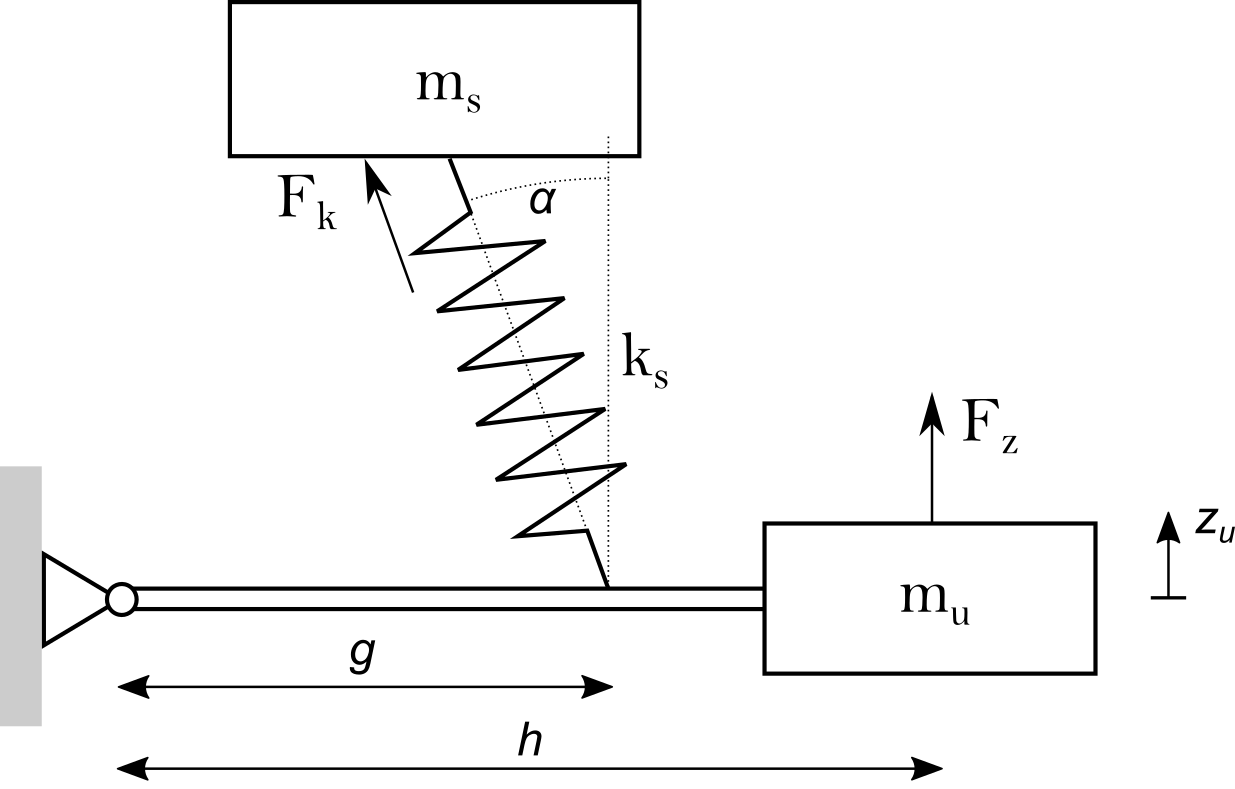
\includegraphics[width=0.5\textwidth]{bilder/suspension.png}
 \caption{The strut equivalent schematic}
 \label{fig:susp}
 \end{figure}

Regardless of the damper, the spring elongation $\delta_u$ is

\begin{equation}
    \delta_u = -\frac{g}{h} cos\alpha \cdot z_u
\end{equation}

According to the spring elongation, the spring force $F_k$ is

\begin{equation}
    F_k = -k_s\delta_u = k_s\frac{g}{h} cos\alpha \cdot z_u
\end{equation}

It is now possible to substitute the tilted spring elongation with an equivalent spring elongation $z_{eq}$ on the z-axis that needs the same force $F_z$, to elongate the same amount as the mass moves.
%

\begin{equation}
    z_{eq} = \frac{g}{h} cos\alpha \cdot z_u
\end{equation}

The vertical component of the force on the unsprung mass can be calculated by

\begin{equation}
    F_z = \frac{g}{h} cos\alpha \cdot F_k
\end{equation}

Thus the relationship can be describe by a equivalent coefficient $i$, the force on the sprung mass $F$ and on the unsprung mass $F_z$ are

\begin{align}
    F &= -cos\alpha \cdot (k_s(z_s - i\cdot z_u)+d_s(\dot{z_s}-i\cdot \dot{z_u})) \\
    F_z &= i\cdot (k_s(z_s - i\cdot z_u)+d_s(\dot{z_s}-i\cdot \dot{z_u}))
\end{align}

where

\begin{equation}
    i = \frac{g}{h} cos\alpha
\end{equation}

The equivalent coefficient $i$ is relative to the dimension of the structure of the suspension.
%
Due to the unavailable devices for the measurement of the length and angle of the strut, the coefficient is temporarily assumed as one.
%
Here i ignore the influence by the mechanic structure of the suspension.

With the above mentioned assumptions the \ac{FCM} is shown in Fig.~\ref{fig:fullcar},

\begin{figure}%
\footnotesize
\centering
\pgfdeclarelayer{bg}    % declare background layer
\pgfsetlayers{bg,main}
\begin{tikzpicture}
%\draw (-8.7,-2.7) rectangle (2,3.7);
\clip (-8.7,-2.7) rectangle (2,3.7);
		\def\lengthstreet{0.6cm};
		\def\spacerstreet{0cm};
		\def\tireheight{0.4cm};
		\def\tirewidth{0.8cm};
		\def\vectorlength{0.39cm};
		\def\labledistanceleft{0.0cm};
		\def\labledistanceright{0.15cm};
		\def\myyshift{-0.19cm}
		
		\def\a{-0.2cm};
		\def\b{-1.3cm};
		\def\c{-2.8cm};
		\def\d{0.21cm};
		\tikzstyle{line}=[];
     \tikzstyle{spring}=[line,decorate,decoration={zigzag,pre length=0.3cm,post length=0.3cm,segment length=6}]
		 
     \tikzstyle{strasse}=[line,decorate,decoration={snake,pre length=0cm,post length=0.0cm,segment length=30, amplitude = 0.1cm}]%, pattern = north east lines] 
     \tikzstyle{dampener}=[line,decoration={markings, mark connection node=dmp,mark=at position 0.5 with {
     \node (dmp) [line,inner sep=0pt,transform shape,rotate=-90,minimum width=15pt,minimum height=3pt,draw=none] {};
     \draw [line] ($(dmp.north east)+(2pt,0)$) -- (dmp.south east) -- (dmp.south west) -- ($(dmp.north west)+(2pt,0)$); \draw [line] ($(dmp.north)+(0,-5pt)$) -- ($(dmp.north)+(0,5pt)$);}}, decorate]
     \tikzstyle{ground}=[fill,pattern=north east lines,draw=none,minimum width=4cm,minimum height=0.3cm]

		\newcommand\centerofmassfc{%
    \tikz[radius=0.4em] {%
        \fill (0,0) -- ++(0.4em,0) arc [start angle=0,end angle=90] -- ++(0,-0.8em) arc [start angle=270, end angle=180];%
        \draw (0,0) circle;%
			}%
		}
     \begin{scope}
		
		
  \coordinate (A0) at (-7cm,0.5cm);% node at (A0){A0}; % central top point (To pick)
	\coordinate (A1) at ($(A0) + (0cm,\a)$);% node at (A1){A1}; % central top point (To pick)
	\coordinate (A3) at ($(A1) + (0cm,\c)$);
	
	
	\coordinate (B0) at (-2.5cm,1.7cm);% node at (B0){B0}; % right vanishing point (To pick)
	\coordinate (B1) at ($(B0) + (0cm,\a)$);% node at (B1){B1}; % right vanishing point (To pick)
	\coordinate (B3) at ($(B1) + (0cm,\c)$);
	
	
	\coordinate (C0) at (0cm,1.7cm);% node at (C0){C0}; % left vanishing point (To pick)
	\coordinate (C1) at ($(C0) + (0cm,\a)$);% node at (C1){C1}; % left vanishing point (To pick)
	\coordinate (C3) at ($(C1) + (0cm,\c)$);
	
	\coordinate (D0) at (-4.5cm,0.5cm);% node at (D0){D0}; % central bottom point (To pick)
	\coordinate (D1) at ($(D0) + (0cm,\a)$);% node at (D1){D1}; % central bottom point (To pick)
	\coordinate (D3) at ($(D1) + (0cm,\c)$);
	
	
	
	

	%% (C1) and (B1) defines the 2 central points of the cuboid

	

%	\node at (barycentric cs:C1=1,B1=1,B1=1,D1=1) {\tiny f6};
	
	\fill[color=white] (D1) .. controls (B0) and (B0)  ..  (B0) .. controls (C1) and (C1) .. (D1);
	
	
	
 \draw[line, <->] ($(B0) + (0cm,0.2cm)$) -- ($(C0)!0.5!(B0)+ (0cm,0.2cm)$) node[midway, above]{$D_r$};
 \draw[line, <->] ($(C0) + (0cm,0.2cm)$) -- ($(C0)!0.5!(B0)+ (0cm,0.2cm)$) node[midway,above]{$D_l$};
	%% (C1) and (B1) defines the 2 central points of the cuboid


	%\draw[thick, <->] ($(A0) + (0cm,0.5cm)$) -- ($(B0) + (0cm,0.5cm)$) node[midway, above] {b};
	\draw[line, <->] ($(A0) + (0cm,0.2cm)$) -- ($(A0)!0.5!(B0)+ (0cm,0.2cm)$) node[midway, above] {$L_f$};
	\draw[line, <->] ($(B0) + (0cm,0.2cm)$) -- ($(A0)!0.5!(B0)+ (0cm,0.2cm)$) node[midway, above] {$L_r$};
%	\draw[thick, <->] (-2.5cm,3cm) -- (2cm,4.5cm) node[midway,above] {b};
	
\draw[very thick, <-] ($(A0)!-0.1!(B0) + (0cm,1.5cm)$) -- ($(A0)!0.3!(B0)+ (0cm,1.5cm)$) node[midway,above] {$ \vec v$};


	
% Vektoren

	\node at ($(barycentric cs:C0=1,B0=1,A0=1,D0=1)+ (0cm,-0.1cm)$)(cg){};

	     \draw [dashed,thick, -latex](cg.center) -- +(0,2) node[right] {$Z$}; % vektor
			\draw [-latex, thick, rotate=0] ($(cg.center) +(0.15,2.2)$) arc [start angle=-70, end angle=250, x radius=0.4cm, y radius=0.06cm] node[above = 0.1cm] {$\psi$ }; 
			
			
       \draw [dashed, thick, -latex](cg.center) -- +(-4.5,-1.2) node[above right, yshift=2] {$X$}; % vektor
			\draw [-latex, thick, rotate=0] ($(cg.center) +(-4.6,-1.05)$) arc [start angle=20, end angle=340, x radius=0.15cm, y radius=0.4cm] node[below = 0.3cm] {$\phi$ }; 
			
			 \draw [dashed,thick, -latex](cg.center) -- +(4.7,-0) node[above left] {$Y$}; % vektor
			\draw [-latex, thick, rotate=0] ($(cg.center) +(4.85,-0.15)$) arc [start angle=200, end angle=530, x radius=0.2cm, y radius=0.4cm] node[below = 0.45cm] {$\theta$ };
			
%\node at (cg)[circle,style={draw,outer sep=0pt,thick, fill = gray!0}]{\tiny M};
			\node at (cg) {\centerofmassfc};
			\node at ($(cg.center) + (0.3,0.3)$) [right]{ M};
			
%			\node at ($(A1)+(1,0)$) {\centerofmassfc};
			
			
			\draw [line](C1) -- (C0);
  		%\draw [line, opacity= 0.4](B1) -- (B0);
  		\draw [line](A1) -- (A0);
  		\draw [line](D1) -- (D0);
  		\draw [line](D1) -- (C1);
  		\draw [line](D1) -- (A1);
  		%\draw [line, opacity= 0.4](B1) -- (A1);
  		%\draw [line, opacity= 0.4](B1) -- (C1);
  		\draw [line](D0) -- (A0);
  		\draw [line](D0) -- (C0);
  		\draw [line](B0) -- (C0);
  		\draw [line](B0) -- (A0);




% Rad unten rechts
%	\node at (barycentric cs:A1=1,D1=1,C0=1,B0=1) {\tiny f3};
%     \node at (2.5,0.5) [draw,rectangle, minimum width=9cm,minimum height=1cm,anchor=south,,transform shape](D2) {$D2$}; %Box D2
%      \draw [very thick, -latex](D2.north) -- +(0,1); % vektor 
		
			\draw [line] ($(D1) + (-\d,-\d)$) -- (D1);
  		\draw [line]($(D1) + (\d,-\d)$) -- (D1);
     \node at ($(D1) + (0cm,\b)$) [rectangle, minimum width=\tirewidth,minimum height=\tireheight,anchor=north,style={draw,outer sep=0pt}](D2) {$m_2$}; %Box C2
     \draw [thick, -latex](D2.north) -- +(0,\vectorlength); % vektor
     \draw [spring] (D2.135) -- ($(D1) + (-\d,-\d)$) node[midway,left=\labledistanceleft, yshift=\myyshift] {$k_2$}; % Feder
      \draw [dampener,label=D1,] (D2.45) -- ($(D1) + (\d,-\d)$)node[midway,right=\labledistanceright, yshift=\myyshift] {$d_2$}; % Dämpfer
%      \node (ground1) at (-2,-5.5)  [ground, anchor=north] {}; % Boden
%        \draw [ground] (-1,-5) -- (1,-5);
      \draw [spring] ($(D3)$) -- (D2.270)node[midway,left=\labledistanceleft, yshift=\myyshift] {$k_{t2}$}; % Feder
%     \draw [spring] (-0.5,-5) -- (-0.5,-3)node[draw=none,midway,left=0.3cm] {k2}; % If you don't want borders around lables use [draw=none]
%       \draw [dampener] (1.5,-6) -- (1.5,-4)node[midway,right=0.4cm] {d2}; %Dämpfer

% Rad oben rechts

 %    \node at (5,0) [draw,rectangle, minimum width=5cm,minimum height=1cm,anchor=south,,transform shape](A2) {$A2$}; %Box D2
 %     \draw [very thick, -latex](A2.north) -- +(0,1); % vektor 
		  \draw [line]($(C1) + (-\d,-\d)$) -- (C1);
  		\draw [line]($(C1) + (\d,-\d)$) -- (C1);
     \node at ($(C1) + (0cm,\b)$) [rectangle, minimum width=\tirewidth,minimum height=\tireheight,anchor=north,style={draw,outer sep=0pt,line}](C2) {$m_4$}; %Box C2
		
     \draw [thick, -latex](C2.north) -- +(0,\vectorlength); % vektor
     \draw [spring] (C2.135) -- ($(C1) + (-\d,-\d)$) node[midway,left=\labledistanceleft, yshift=\myyshift] {$k_4$}; % Feder
      \draw [dampener,label=D1,] (C2.45) -- ($(C1) + (\d,-\d)$)node[midway,right=\labledistanceright, yshift=\myyshift] {$d_4$}; % Dämpfer
 %     \node (ground1) at (7,-2.5)  [ground, anchor=north] {}; % Boden
%        \draw [ground] (-1,-5) -- (1,-5);
      \draw [spring] ($(C3)$) -- (C2.270)node[midway,left=\labledistanceleft, yshift=\myyshift] {$k_{t4}$}; % Feder
%     \draw [spring] (-0.5,-5) -- (-0.5,-3)node[draw=none,midway,left=0.3cm] {k2}; % If you don't want borders around lables use [draw=none]
%       \draw [dampener] (7.5,-3.5) -- (7.5,-1.5)node[midway,right=0.4cm] {d4}; %Dämpfer

% Rad unten links

			\draw [line]($(A1) + (-\d,-\d)$) -- (A1);
  		\draw [line]($(A1) + (\d,-\d)$) -- (A1);
     \node at ($(A1) + (0cm,\b)$) [rectangle, minimum width=\tirewidth,minimum height=\tireheight,anchor=north,style={draw,outer sep=0pt,line}](A2) {$m_1$}; %Box C2
     \draw [thick, -latex](A2.north) -- +(0,\vectorlength); % vektor
     \draw [spring] (A2.135) --($(A1) + (-\d,-\d)$) node[midway,left=\labledistanceleft, yshift=\myyshift] {$k_1$}; % Feder
      \draw [dampener,label=D1,] (A2.45) -- ($(A1) + (\d,-\d)$)node[midway,right=\labledistanceright, yshift=\myyshift] {$d_1$}; % Dämpfer
%      \node (ground1) at (-7,-5.5)  [ground, anchor=north] {}; % Boden
%        \draw [ground] (-1,-5) -- (1,-5);
      \draw [spring] ($(A3)$) -- (A2.270)node[midway,left=\labledistanceleft, yshift=\myyshift] {$k_{t1}$}; % Feder
%     \draw [spring] (-0.5,-5) -- (-0.5,-3)node[draw=none,midway,left=0.3cm] {k2}; % If you don't want borders around lables use [draw=none]
%       \draw [dampener] (-2.5,-2.5) -- (-2.5,-0.5)node[midway,right=0.4cm] {d6}; %Dämpfer

% Rad oben links

\begin{pgfonlayer}{bg}
		  \draw [line, opacity= 1]($(B1) + (-\d,-\d)$) -- (B1);
  		\draw [line, opacity= 1]($(B1) + (\d,-\d)$) -- (B1);
     \node at ($(B1) + (0cm,\b)$) [rectangle, minimum width=\tirewidth,minimum height=\tireheight,anchor=north,style={draw,outer sep=0pt,line}](B2) {$m_3$}; %Box C2
		
     \draw [thick, -latex](B2.north) -- +(0,\vectorlength); % vektor
     \draw [spring, opacity= 1] (B2.135) -- ($(B1) + (-\d,-\d)$) node[midway,left=\labledistanceleft, yshift=\myyshift] {$k_3$}; % Feder
		
      \draw [line,decoration={markings, mark connection node=dmp,mark=at position 0.5 with {
     \node (dmp) [line,inner sep=0pt,transform shape,rotate=-90,minimum width=15pt,minimum height=3pt,draw=none] {};
     \draw [line,opacity = 1] ($(dmp.north east)+(2pt,0)$) -- (dmp.south east) -- (dmp.south west) -- ($(dmp.north west)+(2pt,0)$); \draw [line, opacity = 1] ($(dmp.north)+(0,-5pt)$) -- ($(dmp.north)+(0,5pt)$);}}, decorate, opacity= 1] (B2.45) -- ($(B1) + (\d,-\d)$)node[midway,right=\labledistanceright, yshift=\myyshift] {$d_3$}; % Dämpfer

%      \node (ground1) at (2,-2.5)  [ground, anchor=north] {}; % Boden
%        \draw [ground] (-1,-5) -- (1,-5);
      \draw [spring] ($(B3)$) -- (B2.270)node[midway,left=\labledistanceleft, yshift=\myyshift] {$k_{t3}$}; % Feder
%     \draw [spring] (-0.5,-5) -- (-0.5,-3)node[draw=none,midway,left=0.3cm] {k2}; % If you don't want borders around lables use [draw=none]
%       \draw [dampener] (3.5,-1.5) -- (3.5,0.5)node[midway,right=0.4cm] {d8}; %Dämpfer
\end{pgfonlayer}



			\draw [strasse] ($(A3) + (-\lengthstreet,\spacerstreet)$) -- ($(A3) + (\lengthstreet,\spacerstreet)$) node[midway,right=\lengthstreet] {$r_{1}$};
			\draw [strasse] ($(D3) + (-\lengthstreet,\spacerstreet)$) -- ($(D3) + (\lengthstreet,\spacerstreet)$) node[midway,right=\lengthstreet] {$r_{2}$};
			\draw [strasse] ($(B3) + (-\lengthstreet,\spacerstreet)$) -- ($(B3) + (\lengthstreet,\spacerstreet)$) node[midway,right=\lengthstreet] {$r_{3}$};	
			\draw [strasse] ($(C3) + (-\lengthstreet,\spacerstreet)$) -- ($(C3) + (\lengthstreet,\spacerstreet)$) node[midway,right=\lengthstreet] {$r_{4}$};	
			
			%\draw[strasse, white ,pattern = north east lines,path fading=south] ($(A3)+ (\lengthstreet,\spacerstreet)$) rectangle +(1.2,-2);
			%\draw[ white ,path fading=south,draw=black] ($(A3)+ (5,-4)$) rectangle +(3,3);
			%\draw  (3,-6) -- (3,-3) -- (0,-3) -- (0,-6);
			%\draw[line,decorate,decoration={snake,pre length=0cm,post length=0.0cm,segment length=30, amplitude = 0.1cm}]  (1.2,-3) -- (0,-3) ;
			%\filldraw [thick, fill=red] ($(Origin)+(2,-6)$) coordinate (Square) -- ++(0,4) -- ++(4,0) -- ++(0,-4);
			
			%\coordinate (A) at ($(A3)+ (-\lengthstreet,\spacerstreet)$);
			%\coordinate (B) at ($(A3)+ (\lengthstreet,\spacerstreet)$);
			%\coordinate (C) at ($(A3)+ (\lengthstreet,-\spacerstreet)$);
			%\coordinate (D) at ($(A3)+ (-\lengthstreet,-\spacerstreet)$);
			%\begin{scope}[strasse]
			%	\draw[fill=red,pattern = north east lines,path fading=south,] (B) to (C) 
              %  decorate {-- (D)}  
              %  to (A) 
              %  to (B);
				%\end{scope}
			

			%[line,decorate,decoration={snake,pre length=0cm,post length=0.0cm,segment length=30, amplitude = 0.1cm}]
%			\draw[white ,pattern = north east lines,path fading=south] (-9,-5.63) rectangle +(4,-1.0);
%			\draw[white ,pattern = north east lines,path fading=south] (-4,-5.63) rectangle +(4,-1.0);
%			\draw[white ,pattern = north east lines,path fading=south] (5,-2.63) rectangle +(4,-1.0);
			
			
      \end{scope}	
					
					\node at (-2,4.8)(a){};
					\node at (-0.5,4.8)(b){};
					%\draw [dashed,-latex]($(C1) + (0cm,-1.55cm)$) -- ($(C1) + (2.5cm,-1.55cm)$) node[above  ] {\scriptsize}; % vektor
					%\draw [-latex, thick, rotate=0] (2.8cm,-0.4cm) arc [start angle=-160, end angle=180, x radius=0.3cm, y radius=0.5cm];
					
  				\node at (0.5,4.95)(c){};
					\node at (2,5.5)(d){};
					%\path[very thick, -latex] (d) edge[bend right = 60] node [above = 0.1cm] {Pitch} (c);
\end{tikzpicture}
\caption{Full car model for simulation.}
\label{fig:fullcar}
\end{figure}
 
The definition of the not labeled variables is shown in table~\ref{tbl:def_of_var} and the differential equations of the heaving \eqref{equ:fcm1}, pitching \eqref{equ:fcm2}, rolling \eqref{equ:fcm3} of the vehicle and vertical motion of each wheel \eqref{equ:fcm4} is derived as follows

\begin{table}
\centering
\caption{Definition of the variables}
\label{tbl:def_of_var}
\begin{tabular}{ll} \hline
variables & definition \\ \hline
$z$ & vertical displacement of the vehicle body \\
$z_{si}$ & vertical displacement of the $i$th sprung mass \\
$z_{ui}$ & vertical displacement of the $i$th unsprung mass \\ \hline
\end{tabular}
\end{table}
 
\begin{align}
    %
    M\ddot{z} &=\sum_{i=1}^4-k_{i}(z_{si}-z_{ui})-d_{i}(\dot{z}_{si}-\dot{z}_{ui}) \label{equ:fcm1}, \\ 
    %
    \begin{split}
     J_{yy}\ddot{\theta}&=\sum_{i=1,2}D_f(k_{i}(z_{si}-z_{ui})+d_{i}(\dot{z}_{si}-\dot{z}_{ui}))\\
     &+\sum_{i=3,4}-D_r(k_{i}(z_{si}-z_{ui})+d_{i}(\dot{z}_{si}-\dot{z}_{ui})),
     \end{split} \label{equ:fcm2} \\ 
     %
     \begin{split}
     J_{xx}\ddot{\phi}&=\sum_{i=1,3}L_l(k_{i}(z_{si}-z_{ui})+d_{i}(\dot{z}_{si}-\dot{z}_{ui}))\\
     &+\sum_{i=2,4}-L_r(k_{i}(z_{si}-z_{ui})+d_{i}(\dot{z}_{si}-\dot{z}_{ui})),
     \end{split} \label{equ:fcm3}\\ 
     %
     m_i\ddot{z}_{ui}&=k_{i}(z_{si}-z_{ui})+d_{i}(\dot{z}_{si}-\dot{z}_{ui})-k_{ti}(z_{ui}-r_i). \label{equ:fcm4}
     %
\end{align}

The relation between $z$ and $z_{si}$ is
 \begin{align}
     z_{s_1}&=z-L_f\theta+D_l\phi,\\
     z_{s_2}&=z-L_f\theta-D_r\phi,\\
     z_{s_3}&=z+L_r\theta+D_l\phi,\\
     z_{s_2}&=z+L_f\theta-D_r\phi.
 \end{align}

 The differential equations are transferred into state space representation, which is a compact mathematical model of a physical system as a set of input, output and state variables related by first-order differential equations.
 %
 It replaces $n$ order linear differential equations with a first order matrix differential equation, directly provides a time-domain solution, and is computational efficient.
 \begin{align}
     \dot{x}&=Ax+Bu\\
     y&=Cx+Du 
 \end{align}
 where $x$ is a $14\times1$ state vector which contains the first and second derivative of the vertical, roll and pitch motion, $u$ a $4\times1$ input vector containing the road signal of each wheel. 
 %
 The output variable $y$ is a $3\times1$ vector that contains the response of the vehicle body at vertical, roll and pitch direction.
 %
 The dynamic system is simulated in \textsc{Matlab} with the Control System Toolbox.


%%%%%%%%%%%%%%%%%%%%%%%%%%%%%%%%%%%%%%%%%%%%%%%%%%%%%%%%%%%%%%%%%%%%%%%%%%%%%%%%%%%%%%%%%%%%%%%%%%%
 \section{Transfer function of the Full Car Model}
 \label{sec:tf}
 
 The transfer function is a mathematical function giving the corresponding output value for each possible value of the input to the system.
 %
 It is a good way to simplify the behavior of the vehicle to the road signal, because it is identified only by the the road signal and the accelerations of the vehicle \cite{iliev2014systemansatz}.
 %
 With the Laplace-Transformation the model can be transferred from state space to transfer function.
 
 \begin{align}
    sX(s)&=AX(s)+BU(s)\\
    Y(s)&=CX(s)+DU(s)
 \end{align}
 
 transformed with $X(s)$, the transfer function $G(s)$
 
 \begin{align}
     X(s)&=(s\cdot I - A)^{-1}\cdot B\cdot U(s) \\
     Y(s)&=(C\cdot (s\cdot I - A)^{-1}\cdot B+D)\cdot U(s) \\
     \label{equ:tf}
     G(s)&=C\cdot (s\cdot I -A)^{-1}\cdot B+D
 \end{align}
 
 The element at $i$th row and $j$th column in the transfer function $G_(s)$ is the also the sub transfer function of the $i$th output and the $j$th input.
 
 \begin{equation}
     G_{ij}=\frac{Y_i}{U_j}
 \end{equation}
 
 Hence the full car model can be described as
 
 \begin{equation}
     \begin{bmatrix}
     \ddot{Z}\\
     \ddot{\Theta}\\
     \ddot{\Phi}
     \end{bmatrix}=\begin{bmatrix}
 G_{11} & G_{12} & G_{13} & G_{14}\\
 G_{21} & G_{22} & G_{23} & G_{24}\\
 G_{31} & G_{32} & G_{33} & G_{34}
 \end{bmatrix} \cdot
 \begin{bmatrix}
 R_1\\
 R_2\\
 R_3\\
 R_4
 \end{bmatrix}
 \end{equation}
 
 In this \ac{MIMO} system which has four inputs and three outputs, the lift, pitch and roll motion of the vehicle are resulted by the multiplication of each transfer function $G_{ij}$ and the corresponding road stimulation $r_{j}$.
 %
 Because the value of the variables of the four subset e.g $k_i$, $d_i$ and $k_{ti}$ in the vehicle suspension are symmetrically, after the calculation in formular~\ref{equ:tf}, the amplitude of the sub transfer function in the same row are consequently identical but some phases are shifted.
 %
 The bode phase plot of all the sub transfer functions are shown in Fig.~\ref{fig:sub_tf}.
 %
 The row indicates the four inputs and the column indicates the three outputs.
 
 \begin{figure}
 \centering
 \begin{tikzpicture}
 \begin{groupplot}[mygroupplot,
 group style={group name=my plots,group size= 3 by 4, horizontal sep=\myGroupSep, 
 vertical sep=\myGroupVertSep},
 ]
    %1
    \nextgroupplot[
    xlabel=Frequency ($Hz$),
	ylabel=Phase (deg),
  	ymax=460,   
  	ymin=-180,
  	xmode=log,
  	cycle list name=mycyclelist,
    ]
    \newcommand{\point}{1};
    \addplot+[no marks, each nth point=\point] table[x=f,y=p1] {data/phase_tf.txt};
    %2
    \nextgroupplot[
	xlabel=Frequency ($Hz$),
	ylabel=Phase (deg),
	ymax=460,   
  	ymin=-180,
  	xmode=log,
  	cycle list name=mycyclelist,
    ]
    \newcommand{\point}{1};
    \addplot+[no marks, each nth point=\point] table[x=f,y=p5] {data/phase_tf.txt};
    %3
    \nextgroupplot[
	xlabel=Frequency ($Hz$),
	ylabel=Phase (deg),
	ymax=460,   
  	ymin=-180,
  	xmode=log,
  	cycle list name=mycyclelist,
    ]
    \newcommand{\point}{1};
    \addplot+[no marks, each nth point=\point] table[x=f,y=p9] {data/phase_tf.txt};
    %4
    \nextgroupplot[
	xlabel=Frequency ($Hz$),
	ylabel=Phase (deg),
	ymax=460,   
  	ymin=-180,
  	xmode=log,
  	cycle list name=mycyclelist,
    ]
    \newcommand{\point}{1};
    \addplot+[no marks, each nth point=\point] table[x=f,y=p2] {data/phase_tf.txt};
    %5
    \nextgroupplot[
	xlabel=Frequency ($Hz$),
	ylabel=Phase (deg),
	ymax=460,   
  	ymin=-180,
  	xmode=log,
  	cycle list name=mycyclelist,
    ]
    \newcommand{\point}{1};
    \addplot+[no marks, each nth point=\point] table[x=f,y=p6] {data/phase_tf.txt};
    %6
    \nextgroupplot[
	xlabel=Frequency ($Hz$),
	ylabel=Phase (deg),
	ymax=460,   
  	ymin=-180,
  	xmode=log,
  	cycle list name=mycyclelist,
    ]
    \newcommand{\point}{1};
    \addplot+[no marks, each nth point=\point] table[x=f,y=p10] {data/phase_tf.txt};
    %7
    \nextgroupplot[
	xlabel=Frequency ($Hz$),
	ylabel=Phase (deg),
	ymax=460,   
  	ymin=-180,
  	xmode=log,
  	cycle list name=mycyclelist,
    ]
    \newcommand{\point}{1};
    \addplot+[no marks, each nth point=\point] table[x=f,y=p3] {data/phase_tf.txt};
    %8
    \nextgroupplot[
	xlabel=Frequency ($Hz$),
	ylabel=Phase (deg),
	ymax=460,   
  	ymin=-180,
  	xmode=log,
  	cycle list name=mycyclelist,
    ]
    \newcommand{\point}{1};
    \addplot+[no marks, each nth point=\point] table[x=f,y=p7] {data/phase_tf.txt};
    %9
    \nextgroupplot[
	xlabel=Frequency ($Hz$),
	ylabel=Phase (deg),
	ymax=460,   
  	ymin=-180,
  	xmode=log,
  	cycle list name=mycyclelist,
    ]
    \newcommand{\point}{1};
    \addplot+[no marks, each nth point=\point] table[x=f,y=p11] {data/phase_tf.txt};
    %10
    \nextgroupplot[
	xlabel=Frequency ($Hz$),
	ylabel=Phase (deg),
	ymax=460,   
  	ymin=-180,
  	xmode=log,
  	cycle list name=mycyclelist,
    ]
    \newcommand{\point}{1};
    \addplot+[no marks, each nth point=\point] table[x=f,y=p4] {data/phase_tf.txt};
    %11
    \nextgroupplot[
	xlabel=Frequency ($Hz$),
	ylabel=Phase (deg),
	ymax=460,   
  	ymin=-180,
  	xmode=log,
  	cycle list name=mycyclelist,
    ]
    \newcommand{\point}{1};
    \addplot+[no marks, each nth point=\point] table[x=f,y=p8] {data/phase_tf.txt};
    %12
    \nextgroupplot[
	xlabel=Frequency ($Hz$),
	ylabel=Phase (deg),
	ymax=460,   
  	ymin=-180,
  	xmode=log,
  	cycle list name=mycyclelist,
    ]
    \newcommand{\point}{1};
    \addplot+[no marks, each nth point=\point] table[x=f,y=p12] {data/phase_tf.txt};
 
 \end{groupplot}
 
 \node[below = \myLabelSep of my plots c1r4.south] {(a) heaving};
 \node[below = \myLabelSep of my plots c2r4.south] {(b) pitching};
 \node[below = \myLabelSep of my plots c3r4.south] {(c) rolling};
 
 \end{tikzpicture}
 \label{fig:sub_tf}
 \caption{Bode Phase Plot of All Transfer Functions.}
 \end{figure}
 
 It can be seen that the profile of the phase plots in the same column are identical.
 %
 Besides, the phase of several outputs have a -180\degree~translation, which means those outputs should take the opposite values.
 %
 To simplify the transfer function, we set three new inputs from the combination of the four road signals to match the phase plot of sub transfer functions.
 
 The input for the heaving motion is the sum of all signals.
 \begin{equation}
     U_{heave}=r_1+r_2+r_3+r_4
 \end{equation}
 
 The input for the pitching motion is the difference of front axle and rear axle
 \begin{equation}
     U_{pitch}=r_1+r_2-r_3-r_4
 \end{equation}
 
 The input for the rolling motion is the difference of left side and right side
 \begin{equation}
     U_{roll}=r_1-r_2+r_3-r_4
 \end{equation}
 
 With the new inputs and transfer functions the \ac{MIMO} system is transformed to three \ac{SISO} systems.
 \begin{equation}
     \begin{bmatrix}
     \ddot{Z}\\
     \ddot{\Theta}\\
     \ddot{\Phi}
     \end{bmatrix}=
     \begin{bmatrix}
     G_z & 0 & 0\\
     0 & G_p & 0\\
     0 & 0 & G_r
     \end{bmatrix} \cdot
     \begin{bmatrix}
     U_{heave}\\
     U_{pitch}\\
     U_{roll}
     \end{bmatrix}
 \end{equation}
 
 where 
 \begin{align}
     G_{z}& = G_{11}\\
     G_{p}& = G_{21}\\
     G_{r}& = G_{31}
 \end{align}
 
 
 Fig.~\ref{fig:transfer_function} shows the coherence between the response of the \ac{MIMO} system and \ac{SISO} system with the road profile in~\ref{sec:roadmodel}.
 %
 From the high coherence it is obvious that the results of two systems are almost identical.
 %
 With this method state space representation has been converted to three \ac{SISO} transfer function.
 %
 This conversion makes the analysis of the feature of the full car model in frequency domain easier and can help us to analysis the relation between single output and all the inputs from the four wheels.
 %
 It will be used in section~\ref{sec:antirollbar} and~\ref{sec:positionofoutput}.
 
 \begin{figure}
 \centering
 \begin{tikzpicture}
 \begin{groupplot}[mygroupplot,
 group style={group name=my plots,group size= 3 by 1, horizontal sep=\myGroupSep, 
 vertical sep=\myGroupVertSep},
 ]
 		
 	\nextgroupplot[
	xlabel=Frequency ($Hz$),
	ylabel=Coherence,
	%xmin=27,   
	%xmax=93,
  	%ymin=0.95,   
  	%ymax=1.05,
  	/pgf/number format/precision=5,
% 	legend columns=1,
% 	legend entries={center of gravity, middle of left side},
% 	legend style={at={\myLegendPosition},anchor=south,name=leg},
    cycle list name=mycyclelist,
    ]
    \newcommand{\point}{1};
    \addplot+[no marks, each nth point=\point] table[x=x,y=z1] {data/transfer_function.txt};
    
    \nextgroupplot[
	xlabel=Frequency ($Hz$),
	%ylabel=Coherence,
	%xmin=27,   
	%xmax=93,
    %ymin=0.95,
    %ymax=1.05,
    /pgf/number format/precision=5,
    cycle list name=mycyclelist,
% 	legend columns=1,
% 	legend entries={center of gravity, middle of left side},
% 	legend style={at={\myLegendPosition},anchor=south,name=leg},
    ]
    \newcommand{\point}{1};
    \addplot+[no marks, each nth point=\point] table[x=x,y=z2] {data/transfer_function.txt};
    
    \nextgroupplot[
	xlabel=Frequency ($Hz$),
	%ylabel=Coherence,
	%xmin=27,   
	%xmax=93,
    %ymin=0.95,
    %ymax=1.05,
    /pgf/number format/precision=5,
    cycle list name=mycyclelist,
% 	legend columns=1,
% 	legend entries={center of gravity, middle of left side},
% 	legend style={at={\myLegendPosition},anchor=south,name=leg},
    ]
    \newcommand{\point}{1};
    \addplot+[no marks, each nth point=\point] table[x=x,y=z3] {data/transfer_function.txt};
    
 \end{groupplot}
 \node[below = \myLabelSep of my plots c1r1.south] {(a) heaving};
 \node[below = \myLabelSep of my plots c2r1.south] {(b) pitching};
 \node[below = \myLabelSep of my plots c3r1.south] {(c) rolling};
 \end{tikzpicture}
 \label{fig:transfer_function}
 \caption{Coherence of the response between MIMO- and SISO system}
 \end{figure}




%%%%%%%%%%%%%%%%%%%%%%%%%%%%%%%%%%%%%%%%%%%%%%%%%%%%%%%%%%%%%%%%%%%%%%%%%%%%%%%%%%%%%%%%%%%%%%%%%% 
 \section{Full car model with anti-roll bar}
 \label{sec:antirollbar}
 
 An anti-roll bar, known also as a sway bar, is an commonly used automotive suspension component that elastically couples the suspension on one side of a vehicle to the adjacent side~\cite{doody2013design}.
 %
 It helps to reduce the body roll of a vehicle when the deflection of body and tire between left and right side has a great difference~\cite{iliev2014systemansatz}.
 %
 A sway bar increases the suspension's roll stiffness to rolling motion and is independent of its spring rate in the vertical direction.
 %
 Therefore, the influence of the anti-roll bar should be considered into the full car model.
 %
 The model is shown in Fig.~\ref{fig:arb}.
 

\begin{figure}%
\footnotesize
\centering
\pgfdeclarelayer{bg}    % declare background layer
\pgfsetlayers{bg,main}
\begin{tikzpicture}



		\def\sizecircle{0.25cm};	
		\def\spacerforce{0.2cm};
		\def\force{0.7cm};
		
		
		
		\def\tireheight{0.4cm};
		\def\tirewidth{1.8cm};
		\def\vectorlength{0.39cm};
		\def\labledistanceleft{0.0cm};
		\def\labledistanceright{0.15cm};
		\def\myyshift{-0.19cm}
		\def\myyshiftbig{-0.29cm}
		\def\myyshifty{2pt}
		
		\def\a{3.2cm};
		\def\b{1.0cm};
		\def\c{1.3cm};
		\def\d{1.21cm};
		\def\e{1cm};
		\def\f{1.8cm};
		\tikzstyle{line}=[];
     \tikzstyle{spring}=[line,decorate,decoration={zigzag,pre length=2.8cm,post length=2.8cm,segment length=6}]
		
		 \tikzstyle{suspension}=[line,decoration={markings, mark connection node=dmp,mark=at position 0.5 with {
				\node (dmp) [circle,draw=black,inner sep=0pt,minimum size=0.3cm] {};
				\draw [-latex] ($(dmp) + (-0.16cm,0.22cm)$) -- ($(dmp) + (0.2cm,-0.3cm)$);
				%\draw [fill=white] (dmp) circle (0.18cm);
				%\draw [line] ($(dmp.north east)+(2pt,0)$) -- (dmp.south east) -- (dmp.south west) -- ($(dmp.north west)+(2pt,0)$); \draw [line] ($(dmp.north)+(0,-5pt)$) -- ($(dmp.north)+(0,5pt)$);
				}}, decorate]
		
     \tikzstyle{strasse}=[line,decorate,decoration={snake,pre length=0cm,post length=0.0cm,segment length=30, amplitude = 0.1cm}]%, pattern = north east lines] 
		
     \tikzstyle{dampener}=[line,decoration={markings, mark connection node=dmp,mark=at position 0.5 with {
				\node (dmp) [line,inner sep=0pt,transform shape,rotate=-90,minimum width=15pt,minimum height=3pt,draw=none] {};
				\draw [line] ($(dmp.north east)+(2pt,0)$) -- (dmp.south east) -- (dmp.south west) -- ($(dmp.north west)+(2pt,0)$); \draw [line] ($(dmp.north)+(0,-5pt)$) -- ($(dmp.north)+(0,5pt)$);}}, decorate]
				
     \tikzstyle{ground}=[fill,pattern=north east lines,draw=none,minimum width=4cm,minimum height=0.3cm]

     \begin{scope}
		
		
  \coordinate (A0) at (0,0);% node at (A0){A0}; % central top point (To pick)
	\coordinate (M1) at ($(A0) + (-\a,0)$);% node at (A1){A1}; % central top point (To pick)
	\coordinate (M2) at ($(A0) + (\a,0)$);
	\coordinate (E1) at ($(M1) + (-\b,-\c)$);
	\coordinate (E2) at ($(M2) + (-\b,-\c)$);
	
	\coordinate (B1) at ($(E1) + (\f,0)$);
	\coordinate (B2) at ($(E2) + (-\f,0)$);
	
% Massen
	\node at (M1) [circle,draw=black,fill=black,inner sep=0pt,minimum size=\sizecircle] (mrvr) {};
	\node at (M2) [circle,draw=black,fill=black,inner sep=0pt,minimum size=\sizecircle] (mrvl) {};
    \node at (mrvl) [right=\labledistanceright] {$m_2(m_3)$};
    \node at (mrvr) [right=\labledistanceright] {$m_1(m_4)$};    


% Kräfte	
	\draw [-latex] ($(mrvr) + (0,\force)$) -- ($(mrvr) + (0,\spacerforce)$) node[midway,right=\labledistanceright] {$F_{st}$};
	\draw [-latex] ($(mrvl) + (0,\spacerforce)$) --($(mrvl) + (0,\force)$) node[midway,right=\labledistanceright] {$F_{st}$};
	
	\draw [-latex] ($(B2) + (0,-\force)$) -- ($(B2) + (0,-\spacerforce)$) node[midway,right=\labledistanceright] {$F_{st}\frac{s}{b_{st}}$};
	\draw [-latex] ($(B1) + (0,-\spacerforce)$) --($(B1) + (0,-\force)$) node[midway,left=\labledistanceright] {$F_{st}\frac{s}{b_{st}}$};


\draw [line] (M1) -- (E1) ; 
\draw [line] (E1) -- ($(E1) + (0,-\d)$) ; 

\draw [line] (M2) -- (E2) ; 
\draw [line] (M2) --($(M2) + (0,-\d)$) ; 
\draw [line] (E2) --($(E2) + (0,-\d)$) ; 

\draw [shorten >=0.2cm,shorten <=0.2cm,<->] ($(E1) + (0,-\e)$) --($(E2) + (0,-\e)$) node[midway, yshift=\myyshift] {$s$}; 
\draw [shorten >=0.2cm,shorten <=0.2cm,<->] ($(E2) + (0,-\e)$) --($(M2) + (0,-\e)$) node[midway,right=\labledistanceright, yshift=\myyshiftbig] {$a_{st}$};

\draw [shorten >=0.2cm,shorten <=0.2cm,<->] ($(B1) + (0,0.4)$) --($(B2) + (0,0.4)$) node[midway, yshift=-\myyshift] (bst) {$b_{st}$};

\node at (bst) [yshift=-3em] {$c_{st}$};

\draw [line] ($(B1) + (0,0.1cm)$) --($(B1) + (0,0.6cm)$) ; 
\draw [line] ($(B2) + (0,0.1cm)$) --($(B2) + (0,0.6cm)$) ; 

\draw [line] ($(B1) + (-0.2cm,0.1cm)$) --($(B1) + (0.2cm,0.1cm)$) ; 
\draw [line] ($(B2) + (-0.2cm,0.1cm)$) --($(B2) + (0.2cm,0.1cm)$) ;

\draw [line] ($(B1) + (-0.2cm,-0.1cm)$) --($(B1) + (0.2cm,-0.1cm)$) ; 
\draw [line] ($(B2) + (-0.2cm,-0.1cm)$) --($(B2) + (0.2cm,-0.1cm)$) ;

\draw [spring] (E1) --(E2) node[midway,yshift=\myyshiftbig] {}; % Feder





% Rad unten links

 %    \node at ($(A1) + (0,-\d)$) [rectangle, minimum width=\tirewidth,minimum height=\tireheight,anchor=south,style={draw,outer sep=0pt,line}](A4) {$m_s$}; %Box C2
 %    \node at ($(A1) + (0cm,\b)$) [rectangle, minimum width=\tirewidth,minimum height=\tireheight,anchor=north,style={draw,outer sep=0pt,line}](A2) {$m_u$}; %Box C2
%     \draw [thick, -latex](A2.north) -- +(0,\vectorlength); % vektor
%     \draw [spring] (A2.165) --(A4.195) node[midway,left=\labledistanceleft, yshift=\myyshift] {$k_s$}; % Feder
 %     \draw [dampener,label=D1,] (A2) -- (A4)node[midway,right=\labledistanceright, yshift=\myyshift] {$c_s$}; % Dämpfer
	%		\draw [suspension] (A2.15) --(A4.345) node[midway,right=\labledistanceright, yshift=\myyshift] {$f_s$}; % active suspension
%      \node (ground1) at (-7,-5.5)  [ground, anchor=north] {}; % Boden
%        \draw [ground] (-1,-5) -- (1,-5);
 %     \draw [spring] ($(A3)$) -- (A2)node[midway,left=\labledistanceleft, yshift=\myyshift] {$k_{t}$}; % Feder
			


	%		\draw [strasse] ($(A3) + (-\lengthstreet,\spacerstreet)$) -- ($(A3) + (\lengthstreet,\spacerstreet)$) node[midway,right=\lengthstreet] {$r$};

			
      \end{scope}	
					
\end{tikzpicture}
 \caption{Model of anti-roll bar as a torsion bar between two unsprung masses.}
 \label{fig:arb}%
\end{figure}
 
 
 It connects left and right wheels together through short lever arms linked by a torsion spring whose stiffness is indicated as $c_{st}$.
 %
 The force $F_{st}$ is generated by anti-roll bar to the tire at front and rear axle \eqref{equ:ar3} and anti-roll moment $M_{st}$ to the body \eqref{equ:ar4} are:
 \begin{align}
     \begin{split}
     F_{st,f}&=\pm{\frac{c_{st,f}}{a_{st,f}^2}(z_{s1}-z_{u1}-z_{s2}+z_{u2})}\\
     F_{st,r}&=\pm{\frac{c_{st,r}}{a_{st,r}^2}(z_{s3}-z_{u3}-z_{s4}+z_{u4})}, 
    \end{split} \label{equ:ar3}\\
     M_{st}&=s\frac{c_{st}}{a_{st}^2}(z_{s1}-z_{u1}-z_{s2}+z_{u2})+s\frac{c_{st}}{a_{st}^2}(z_{s3}-z_{u3}-z_{s4}+z_{u4}). \label{equ:ar4}
 \end{align}
 
 According to the additional forces and moments generated by the anti-roll bar, the rolling motion of the vehicle body \eqref{equ:ar1} and vertical motion of each wheel \eqref{equ:ar2} should be reformed:
 
 \begin{align}
     \begin{split}
     J_{xx}\ddot{\phi}&=-M_{st}+\sum_{i=1,3}-L_l(k_{i}(z_{si}-z_{ui})+d_{i}(\dot{z}_{si}-\dot{z}_{ui}))\\
     &+\sum_{i=2,4}L_r(k_{i}(z_{si}-z_{ui})+d_{i}(\dot{z}_{si}-\dot{z}_{ui})),
     \end{split} \label{equ:ar1}\\
     %
     m_i\ddot{z}_{ui}&=k_{i}(z_{si}-z_{ui})+d_{i}(\dot{z}_{si}-\dot{z}_{ui})-k_{ti}(z_{ui}-r_i)+F_{st,i}. \label{equ:ar2}
 \end{align}

 The comparison of the response and transfer function which is already introduced in Sec.~\ref{sec:tf} from road deflection $u_{roll}$ to body roll acceleration $\ddot{\phi}$ of the full car model without and with anti-roll bar are shown in Fig. \ref{fig:anti_roll_bar}.
 %
 The setting of parameters in those simulations are shown in table~\ref{tbl:par_arb.vs.fcm}.

 \begin{table}
 \centering
 \caption{Parameter of the simulation}
 \label{tbl:par_arb.vs.fcm}
 \begin{tabular}{ccccccccc}
 \hline
 $L$ & $D$ & $M$ & $k$ & $d$ & $m_{tire}$ & $k_{tire}$ & $a_{st}$ & $c_{st}$\\ 
 $[m]$ & $[m]$ & $[kg]$ & $[N/m]$ & $[N\cdot s/m]$ & $[kg]$ & $[N/m]$ & $[m]$ & $[N\cdot m]$ \\ \hline
 2.69 & 1.71 & 1400 & 150000 & 2500 & 22.5 & 36689/35902 & 0.2 & 100 \\ \hline
 \end{tabular}
 \end{table}

 It indicates that the roll acceleration is reduced and the magnitude of the transfer function is lower in the range from 10 to 100$Hz$ with the influence of the anti-roll bar.
 %
 That is to say, the results of the simulation of rolling motion with the full car model without the anti-roll bar may be stretched.
 %
 For the reliability and accuracy of the simulation, we add the anti-roll bar to the full car model.

 \begin{figure}
 \centering
 \begin{tikzpicture}
 \begin{groupplot}[mygroupplot,
 group style={group name=my plots,group size= 2 by 1, horizontal sep=\myGroupSep, 
 vertical sep=\myGroupVertSep},
 ]
 		
 	\nextgroupplot[
	xlabel=Distance (\si{\meter}),
	ylabel=Roll acceleration ($rad/s^2$),
	%xmin=27,   
	%xmax=93,
	%ymin=100,   
	%ymax=120,
	legend columns=2,
	legend entries={without anti-roll bar, with anti-roll bar},
	legend style={at={(1.2,1.03)},anchor=south,name=leg},
	cycle list name=mycyclelist,
    ]
    \newcommand{\point}{10};
    \addplot+[no marks, each nth point=\point] table[x=x,y=y1] {data/anti_roll_bar_time_domain.txt};
    \addplot+[no marks, each nth point=\point] table[x=x,y=y2] {data/anti_roll_bar_time_domain.txt};
 
  	\nextgroupplot[
	xlabel=Frequency ($Hz$),
	ylabel=Magnitude ($dB$),
	xmode=log,
	%ymode=log,
	%xmin=,   
	%xmax=,
	%ymin=100,   
	%ymax=120,
	cycle list name=mycyclelist,
    ]
    \newcommand{\point}{1};
    \addplot+[no marks, each nth point=\point] table[x=w,y=a1] {data/bode_plot.txt};
    \addplot+[no marks, each nth point=\point] table[x=w,y=a2] {data/bode_plot.txt};
 
 
 \end{groupplot}
 \end{tikzpicture}
 \caption{Influence of the anti-roll bar. The roll acceleration is distinct reduced as well as the magnitude of the transfer function for lower frequencies.}
 \label{fig:anti_roll_bar}
 \end{figure}




%%%%%%%%%%%%%%%%%%%%%%%%%%%%%%%%%%%%%%%%%%%%%%%%%%%%%%%%%%%%%%%%%%%%%%%%%%%%%%%%%%%%%%%%%%%%%%%%%%%
\section{Full car model with active suspension}
\label{sec:active full car model}

In addition to the passive suspension with basic springs and dampers, active suspensions use separate actuators between the chassis and wheel assembly, which can exert an independent force on the suspension in order to improve the driving comfort.

Ideally, a control action may be introduced at different levels of the suspension system: at the level of the dissipative unit, by a modulation of the damping force; at the level of the elastic unit, by a modulation of the spring force; at the full level of the suspension, by replacing both the elastic and the damping devices with a force actuator.
%
More specifically, three features may be observed: the control ability range which is the range of forces that the actuators can deliver; the control bandwidth which is a measure of how fast the actuator action is; the power request that is mainly due to the mix of control ability range and control bandwidth~\cite{savaresi2010semi}.

Due to the relatively vast range of deliverable forces, in principle, active suspensions may provide the best performance.
%
The active suspension is characterized by its ability to use external energy and usually involves hydraulic components.


% \subsection{semi active suspension}

% Semi-active suspensions generally include a damper whose friction coefficient is always positive, variable (continuously or not) and controlled.
% %
% The semi-active damper can then dissipate energy but cannot deliver additional force using external energy.
% %
% Control of the chassis and the wheel can be achieved by the choice of the damping coefficient in real-time.

% The behavior of the suspension is modelled as:

% \begin{align}
%     %
%     M\ddot{z} &=\sum_{i=1}^4-k_{i}(z_{si}-z_{ui})-u_i \\ 
%     %
%     \begin{split}
%      J_{yy}\ddot{\theta}&=\sum_{i=1,2}D_f(k_{i}(z_{si}-z_{ui})+u_i)\\
%      &+\sum_{i=3,4}-D_r(k_{i}(z_{si}-z_{ui})+u_i),
%      \end{split}\\ 
%      %
%      \begin{split}
%      J_{xx}\ddot{\phi}&=\sum_{i=1,3}L_l(k_{i}(z_{si}-z_{ui})+u_i)\\
%      &+\sum_{i=2,4}-L_r(k_{i}(z_{si}-z_{ui})+u_i),
%      \end{split}\\ 
%      %
%      m_i\ddot{z}_{ui}&=k_{i}(z_{si}-z_{ui})+u_i-k_{ti}(z_{ui}-r_i)
%      %
% \end{align}

% where $u_i$ is the force produced by the damper, which is determined by the variable damping coefficient and relative velocity.

% Skyhook control is one of the classical control for semi-active suspension systems and is most widely used for the suspension control since it represents a simple way to achieve a good comfort requirement~\cite{article}.
% %
% In the principle of this approach the chassis is "linked" to the sky in order to reduced the vertical oscillations of the chassis and of the axle independently of each other~\cite{savaresi2010semi}.
% %
% The general representation of the Skyhook suspension is in the Fig%~\ref{}.

% % bild hier

% This behaviour of the Skyhook can be represented as

% \begin{align}
%     %
%     M\ddot{z} &=\sum_{i=1}^4-k_{i}(z_{si}-z_{ui})-d_{sky}\dot{z}_{si}+\alpha d_i\dot{z}_{ui} \\ 
%     %
%     \begin{split}
%      J_{yy}\ddot{\theta}&=\sum_{i=1,2}D_f(k_{i}(z_{si}-z_{ui})+u_i)\\
%      &+\sum_{i=3,4}-D_r(k_{i}(z_{si}-z_{ui})+u_i),
%      \end{split}\\ 
%      %
%      \begin{split}
%      J_{xx}\ddot{\phi}&=\sum_{i=1,3}L_l(k_{i}(z_{si}-z_{ui})+u_i)\\
%      &+\sum_{i=2,4}-L_r(k_{i}(z_{si}-z_{ui})+u_i),
%      \end{split}\\ 
%      %
%      m_i\ddot{z}_{ui}&=k_{i}(z_{si}-z_{ui})+u_i-k_{ti}(z_{ui}-r_i)
%      %
% \end{align}

% \subsection{fully active suspension}

One fourth of the full car model with active suspension is shown in Fig.~\ref{fig:fcm_as}.
%
The force $f_i$ applied between the body and wheel assembly is generated by a hydraulic actuator and controlled by the feedback in the closed loop.
 
 \begin{figure}%
 \footnotesize
 \centering
 \pgfdeclarelayer{bg}    % declare background layer
\pgfsetlayers{bg,main}
\begin{tikzpicture}
		\def\lengthstreet{0.6cm};
		\def\spacerstreet{0cm};
		\def\tireheight{0.4cm};
		\def\tirewidth{1.8cm};
		\def\vectorlength{0.39cm};
		\def\labledistanceleft{0.0cm};
		\def\labledistanceright{0.15cm};
		\def\myyshift{-0.19cm}
		\def\myyshifty{2pt}
		
		\def\a{-0.2cm};
		\def\b{-1.3cm};
		\def\c{-2.8cm};
		\def\d{0.21cm};
		
		\tikzstyle{line}=[];
     \tikzstyle{spring}=[line,decorate,decoration={zigzag,pre length=0.3cm,post length=0.3cm,segment length=6}]
		
		 \tikzstyle{suspension}=[line,decoration={markings, mark connection node=dmp,mark=at position 0.5 with {
				\node (dmp) [circle,draw=black,inner sep=0pt,minimum size=0.3cm] {};
				\draw [-latex] ($(dmp) + (-0.16cm,0.22cm)$) -- ($(dmp) + (0.2cm,-0.3cm)$);
				%\draw [fill=white] (dmp) circle (0.18cm);
				%\draw [line] ($(dmp.north east)+(2pt,0)$) -- (dmp.south east) -- (dmp.south west) -- ($(dmp.north west)+(2pt,0)$); \draw [line] ($(dmp.north)+(0,-5pt)$) -- ($(dmp.north)+(0,5pt)$);
				}}, decorate]
		
     \tikzstyle{strasse}=[line,decorate,decoration={snake,pre length=0cm,post length=0.0cm,segment length=30, amplitude = 0.1cm}]%, pattern = north east lines] 
		
     \tikzstyle{dampener}=[line,decoration={markings, mark connection node=dmp,mark=at position 0.5 with {
				\node (dmp) [line,inner sep=0pt,transform shape,rotate=-90,minimum width=15pt,minimum height=3pt,draw=none] {};
				\draw [line] ($(dmp.north east)+(2pt,0)$) -- (dmp.south east) -- (dmp.south west) -- ($(dmp.north west)+(2pt,0)$); \draw [line] ($(dmp.north)+(0,-5pt)$) -- ($(dmp.north)+(0,5pt)$);}}, decorate]
				
     \tikzstyle{ground}=[fill,pattern=north east lines,draw=none,minimum width=4cm,minimum height=0.3cm]

    \begin{scope}
		
		
    \coordinate (A0) at (0,0);% node at (A0){A0}; % central top point (To pick)
	\coordinate (A1) at ($(A0) + (0cm,\a)$);% node at (A1){A1}; % central top point (To pick)
	\coordinate (A3) at ($(A1) + (0cm,\c)$);
	\coordinate (U) at ($(A0) + (1cm,-1cm)$);

% Rad unten links

    \node at ($(A1) + (0,-\d)$) [rectangle, minimum width=\tirewidth,minimum height=\tireheight,anchor=south,style={draw,outer sep=0pt,line}](A4) {$M$}; %Box C2
    \node at ($(A1) + (0cm,\b)$) [rectangle, minimum width=\tirewidth,minimum height=\tireheight,anchor=north,style={draw,outer sep=0pt,line}](A2) {$m_u$}; %Box C2
    \node at ($(A1) + (3.7cm,-0.5cm)$) [rectangle, minimum width=0.9cm,minimum height=0.6cm,anchor=north,style={draw,outer sep=0pt,line}](R) {$controller$};
    \node at ($(A1) + (1.7cm,-\d)$) [rectangle, minimum width=0.8cm,minimum height=\tireheight,anchor=south,style={draw,outer sep=0pt,line}](S1) {$sensor$};
    \node at ($(A1) + (1.7cm,\b)$) [rectangle, minimum width=0.8cm,minimum height=\tireheight,anchor=north,style={draw,outer sep=0pt,line}](S2) {$sensor$};
     
%     \draw [thick, -latex](A2.north) -- +(0,\vectorlength); % vektor
    \draw [spring] (A2.165) --(A4.195) node[midway,right=\labledistanceleft, yshift=\myyshift] {$k_s$}; % Feder
    \draw [dampener,label=D1,] (A2) -- (A4)node[midway,right=\labledistanceright, yshift=\myyshift] {$c_s$}; % Dämpfer
	\draw [suspension] (A2.15) --(A4.345) node[midway,right=\labledistanceright, yshift=\myyshift] {$f_i$}; % active suspension
%      \node (ground1) at (-7,-5.5)  [ground, anchor=north] {}; % Boden
%        \draw [ground] (-1,-5) -- (1,-5);
    \draw [spring] ($(A3)$) -- (A2)node[midway,right=\labledistanceleft, yshift=\myyshift] {$k_{t}$}; % Feder
	\draw [strasse] ($(A3) + (-\lengthstreet,\spacerstreet)$) -- ($(A3) + (\lengthstreet,\spacerstreet)$) node[midway,right=\lengthstreet] {$r$};
	
 	\draw [->] (S1) node [above,xshift=1cm] {$\ddot{z_{s}}$} -| (R);
 	\draw [->] (S2) node [above,xshift=1cm] {$z_{u}$} -| (R);
	
 	\draw [->] (R.west) -- node[above]{$u$}(U);

			
    \end{scope}	
					
\end{tikzpicture}
 \caption{One fourth of the full car model with active suspension.}
 \label{fig:fcm_as}%
 \end{figure}
 
 With this model the mathematical modeling for heaving \eqref{equ:afcm1}, pitching \eqref{equ:afcm2}, rolling \eqref{equ:afcm3} of the vehicle body and vertical motion of each wheel \eqref{equ:afcm4} is derived as follows:
 
 \begin{align}
     M\ddot{z}&=\sum_{i=1}^4-k_{ui}(z_{si}-z_{ui})-c_{ui}(\dot{z}_{si}-\dot{z}_{ui})+f_i, \label{equ:afcm1} \\
          \begin{split}
     J_{yy}\ddot{\theta}&=\sum_{i=1,2}L_f(k_{ui}(z_{si}-z_{ui})+c_{ui}(\dot{z}_{si}-\dot{z}_{ui})-f_i)\\
     &+\sum_{i=3,4}-L_r(k_{ui}(z_{si}-z_{ui})+c_{ui}(\dot{z}_{si}-\dot{z_{ui}})-f_i),
     \end{split} \label{equ:afcm2}\\
          \begin{split}
     J_{xx}\ddot{\phi}&=\sum_{i=1,3}D_l(k_{ui}(z_{si}-z_{ui})+c_{ui}(\dot{z}_{si}-\dot{z}_{ui})-f_i)\\
     &+\sum_{i=2,4}-D_r(k_{ui}(z_{si}-z_{ui})+c_{ui}(\dot{z}_{si}-\dot{z}_{ui})-f_i),
     \end{split} \label{equ:afcm3} \\
     m_i\ddot{z}_{ui} &=k_{ui}(z_{si}-z_{ui})+c_{ui}(\dot{z}_{si}-\dot{z}_{ui})-k_{ti}(z_{ui}-r_i)-f_i. \label{equ:afcm4}
 \end{align}
 
There has been a lot of research in the design of a suitable control strategy for the active suspension.
%
For instance, in~\cite{5069178} three different control designs, PI, \ac{LQR} and $H\infty$ were compared for stability, performance and robustness. 
%
Different advanced controllers have also been compared in several studies such as~\cite{5937197} and~\cite{doi:10.1076/vesd.39.4.279.14149}, where \ac{LQR}, Fuzzy, Skyhook and $H\infty$ controllers were tested. 
 
The \ac{LQR} approach of vehicle suspension control is widely used in background of many studies in vehicle suspension control.
%
The strength of LQR approach is that in using it the factors of the performance index can be weighted according to the designer’s desires or other constraints~\cite{agharkakli2012simulation}.
 
The system can be expressed in the state space representation.
%
State variable $x(t)$ is a $14\times1$ vector, input variable $u$ is a $4\times1$ vector which contain the road signal of each wheels and $f$ is the generated forces by actuator under the controller. 
 
 \begin{equation}
     \dot{x}(t)=Ax(t)+B_1u(t)+B_2r(t)
 \end{equation}
 
It it assumed that all the states are measurable and consider a \ac{SVFB} regulator for the system as $u(t)=-Kx(t)$.
%
With the state feedback gain matrix $K$ the closed-loop system is reformed as
 
 \begin{equation}
     \dot{x}(t)=(A-B_1K)x(t)+B_2r(t)
 \end{equation}

 \begin{figure}
 \footnotesize
 \centering
 \begin{tikzpicture}[auto, node distance=2cm,>=latex']

    \tikzstyle{block} = [draw, fill=none, rectangle, 
        minimum height=3em, minimum width=6em]
    \tikzstyle{sum} = [draw, fill=none, circle, node distance=2cm]
    \tikzstyle{input} = [coordinate]
    \tikzstyle{output} = [coordinate]

    \node [input, name=input] {};
    \node [block, right of=input] (B2) {$B_2$};
    \node [block, below of=B2, node distance=1.1cm] (B1) {$B_1$};
    \node [sum, right of=B1] (sum) {};
    \node [block, right of=sum] (integrate) {$\frac{1}{s}$};
    \node [block, below of=integrate, node distance=1.1cm] (A) {$A$};
    \node [block, below of=A, node distance=1.1cm] (K) {$K$};
    \node [output, right of=integrate, node distance=3cm] (output) {};

    \draw [->] (input) -- node {$r$} (B2);
    \draw [->] (B2) -| (sum);
    \draw [->] (B1) -- (sum);
    \draw [->] (sum) -- (integrate);
    \draw [->] (integrate) -- node [name=x] {$x$}(output);
    \draw [->] (x) |- (A);
    \draw [->] (A) -| (sum);
    \draw [->] (x) |- (K);
    \draw [->] (K) -| node [near end] {$u$}(B1);

 \end{tikzpicture}
 \caption{Block diagram of the \ac{LQR}.}
 \label{fig:lqr}%
 \end{figure}

The block diagram of the system is shown in Fig.~\ref{fig:lqr}.
%
Set $A_c = A-B_1K$ and $B_c = B_2$, the system can be presented in state space as
 
 \begin{align}
     \dot{x}(t)&=A_cx(t)+B_cr(t)\\
     y(t)&=Cx(t)+Dr(t)
 \end{align}
 
The optimal controller of given system is defined as controller design which minimizes the following cost-function.
 
 \begin{equation}
 \label{equ:lqr_cost}
     J=\frac{1}{2}\int_{0}^{\infty}(x(t)^TQx(t)+u(t)^TRu(t))dt
 \end{equation}

Linear optimal control theory provides the solution of Eq.~\ref{equ:lqr_cost}.
%
The gain matrix $K$ is computed from,

\begin{equation}
    K = R^{-1}B_1^{T}P
\end{equation}
 
There are a numerical procedures for solving the restrictions. \textsc{Matlab} routine that performs this operation is $lqr (A,B,Q,R)$.
 
where $Q$ and $R$ are positive definite weighting matrices.
%
The two matrices are selected by the design engineer.
%
There are a numerical procedures for solving the restrictions. \textsc{Matlab} routine that performs this operation is $lqr (A,B,Q,R)$.
Depending on how these design parameters are selected, the closed-loop system will exhibit a different response.
%
Larger values of $Q$ generally result in the poles of the closed-loop system matrix $Ac$ being further left in the s-plane so that the state decays faster to zero.
%
larger $R$ means that less control effort is used, so that the poles are generally slower, resulting in larger values of the state $x(t)$~\cite{agharkakli2012simulation}.
 
With the new state space representation we can build the model of the \ac{FCM} with active suspension using the \ac{LQR} controller.

However, since much of the intuitive insight about the effects of controller parameter modification gets lost in the \ac{LQR} designs, the methods include no robustness specification. 
%
It was shown in \cite{doi:10.1076/vesd.39.4.279.14149} that the $H\infty$ control design yields a superior controller that has significantly better stability and performance robustness as compared to classical designs as the design takes the performance specifications into account through the weighting functions.
%
Most often the $H\infty$ based methods have achieved the best results and point out that the efficiency of $H\infty$ control theory seems to be a good choice for active suspension control, which is widely used in the automotive industry because of its low cost and simplicity~\cite{savaresi2010semi}.
%
Hence the $H\infty$ controller is implemented as the force controller in the full car model with active suspension.

$H\infty$ control is design in term of feasibility of certain delay dependent matrix inequalities.
%
It confirms that $H\infty$ control of active suspension system using the optimization of either a weighted single objective functional with hard constrains or multi-objective functional is an effective way to deal with the conflicting vehicle suspension performance problem~\cite{shariati2004decentralized}.

$H\infty$ control is formulated using the general control configuration in Fig.~\ref{fig:Hinf} where $P(s)$ is a linear system given as follows:

 \begin{figure}
 \footnotesize
 \centering
 % \includegraphics[width=0.3\textwidth]{bilder/H_inf.png}
 \begin{tikzpicture}[auto, node distance=2cm,>=latex']

	\tikzstyle{block} = [draw, fill=none, rectangle, 
  		minimum height=5em, minimum width=8em]
	\tikzstyle{point} = [coordinate]

    \node [point, name = input] {};
    \node [point, right of = input, node distance=5em] (p1) {};
    \node [point, below of = p1, node distance=0.5cm] (p2) {};
    \node [point, right of = p1, node distance=8em] (p3) {};
    \node [point, right of = p2, node distance=8em] (p4) {};
    \node [point, right of = p3, node distance=5em] (output) {};
    
    \node [block, below right = -2em and 5em of input, node distance=2cm] (p) {$P$};
    \node [block, below of = p, node distance=2.5cm] (k) {$K$};
    
    \draw [->] (input) -- node {$w$} (p1);
    \draw [->] (k) --++(-2.7,0) node(lowerleft){} |- node [near end] {$u$} (p2);
    \draw [->] (p3) -- node {$e$} (output);
    \draw [->] (p4) -|++(1.5,0) node(lowerright){} |- node [above,xshift=-1cm] {$y$} (k);
    
 \end{tikzpicture}
 \caption{Control configuration of $H\infty$ control.}
 \label{fig:Hinf}
 \end{figure}

\begin{equation}
     \begin{bmatrix}
     e \\
     y 
     \end{bmatrix}= 
     \begin{bmatrix}
    P_{11} & P_{12} \\
    P_{21} & P_{22} 
     \end{bmatrix}
    \begin{bmatrix}
     w\\
     u
 \end{bmatrix}
 \end{equation}

where $w$ is the exogenous input vector, $u$ is the control input vector, $e$ is the controlled output vector and $y$ is the measurement vector.
%
The control design is to find a controller $K(s)$ for a generalized plant $P(s)$ such that, based on the information given by $y$, the control signal $u=K(s)y$ ensures internal stability of the closed-loop system and counteracts the influence of $w$ on $e$, thereby minimizing the closed-loop transfer norm from the exogenous inputs $w$ to the controlled outputs $e$~\cite{doi:10.1076/vesd.39.4.279.14149}.

Given $\gamma$, a prespecified attenuation level.
%
The $H\infty$ control is to desgin a controller that internally stabilizes the closed-loop system and ensures:

\begin{equation}
 ||T_{ew}(s)||_{\infty} = max~\overline{\sigma}(T_{ew}(jw)) \leq \gamma
\end{equation}

where

\begin{equation}
T_{ew}(s)=P_{12}K(s)(I-P_{22}(s)K(s))^{-1}P_{21}(s)+P_{11}(s)
\end{equation}

is the closed-loop transfer matrix from $w$ to $e$ and $\sigma(T_{ew}(jw))$ is the maximal singular value of $T_{ew}(jw)$.

The closed-loop of the active suspension with $H\infty$ control is shown in Fig.~\ref{fig:fcm_Hinf}.

 \begin{figure}
 \footnotesize
 \centering
 %\includegraphics[width=0.5\textwidth]{bilder/fcm_hinf.png}
 \begin{tikzpicture}[auto, node distance=2cm,>=latex']

	\tikzstyle{block1} = [draw, fill=none, rectangle, 
  		minimum height=15em, minimum width=10em]
	\tikzstyle{block2} = [draw, fill=none, rectangle, 
    	minimum height=15em, minimum width=8em]
	\tikzstyle{sblock} = [draw, fill=none, rectangle, 
    	minimum height=3em, minimum width=4em]
	\tikzstyle{sum} = [draw, fill=none, circle, node distance=1cm]
	\tikzstyle{connect} = [draw, fill=black, circle, inner sep=0pt, node distance=0.1cm]
	\tikzstyle{input} = [coordinate]
	\tikzstyle{output} = [coordinate]

    \node [input, name = input] {};
    \node [block1, below right = -2.5em and 12em of input,node distance=6cm] (fcm) {Full car model};
    \node [block2, below of=fcm,node distance=5cm] (k) {K};
    \node [sblock, below left = -4em and 4em of fcm, node distance=2.5cm] (act) {$Actuator$};
    \node [sblock, below of = act] (Wa) {$W_{act.}$};   
    \node [sblock, above right = -3em and 10em of fcm, node distance=2.5cm] (Wz) {$W_{heave}$};
    \node [sblock, above right = -7em and 10em of fcm, node distance=2.5cm] (Wr) {$W_{roll}$};
    \node [sblock, below right = -7em and 10em of fcm, node distance=2.5cm] (Wp) {$W_{pitch}$};
    \node [sblock, below right = -3em and 10em of fcm, node distance=2.5cm] (Wd) {$W_{def.}$};
    \node [sblock, above right = -3em and 11.5em of k, node distance=2.5cm] (W1) {$W_1$};
    \node [sblock, above right = -7em and 11.5em of k, node distance=2.5cm] (W2) {$W_2$};
    \node [sblock, below right = -7em and 11.5em of k, node distance=2.5cm] (W3) {$W_3$};
    \node [sblock, below right = -3em and 11.5em of k, node distance=2.5cm] (W4) {$W_4$};
    \node [sum, left of = W1, node distance=3.6cm] (sum1) {};
    \node [sum, left of = W2, node distance=2.9cm] (sum2) {};
    \node [sum, left of = W3, node distance=2.2cm] (sum3) {};
    \node [sum, left of = W4, node distance=1.5cm] (sum4) {};
    \node [output, right of = Wa] (e1) {$e_1$};
    \node [output, left of = sum1, node distance=0.5cm] (a1) {};
    \node [output, left of = sum2, node distance=1.2cm] (a2) {};
    \node [output, left of = sum3, node distance=1.9cm] (a3) {};
    \node [output, left of = sum4, node distance=2.6cm] (a4) {};
    \node [output, right of = W1] (d1) {};
    \node [output, right of = W2] (d2) {};
    \node [output, right of = W3] (d3) {};
    \node [output, right of = W4] (d4) {};
    \node [output, right of = Wz] (e2) {};
    \node [output, right of = Wr] (e3) {};
    \node [output, right of = Wp] (e4) {};
    \node [output, right of = Wd] (e5) {};
    \node [output, left of = Wz, node distance=3.6cm] (z) {};
    \node [output, left of = Wr, node distance=3.6cm] (r) {};
    \node [output, left of = Wp, node distance=3.6cm] (p) {};
    \node [output, left of = Wd, node distance=3.6cm] (d) {};
    \node [connect, above of = sum1, minimum size=0.1cm, node distance = 5cm] (c1) {};
    \node [connect, above of = sum2, minimum size=0.1cm, node distance = 5cm] (c2) {};
    \node [connect, above of = sum3, minimum size=0.1cm, node distance = 5cm] (c3) {};
    \node [connect, above of = sum4, minimum size=0.1cm, node distance = 5cm] (c4) {};
    
    \draw [draw,->] (input) -- node {$\vec{w}$} (fcm.495);
    \draw [->] (k)--++(-5,0) node(lowerleft){} |- node [near end, name = u] {$\vec{u}$} (act);
    \draw [->] (lowerleft) |- (Wa);
    \draw [->] (Wa) -- node {$\vec{e_1}$} (e1);
    \draw [->] (act) -- node {$\vec{f}$} (fcm.-135);
    \draw [->] (sum1) -- node {$y_1$} (a1);
    \draw [->] (sum2) -- node {$y_2$} (a2);
    \draw [->] (sum3) -- node {$y_3$} (a3);
    \draw [->] (sum4) -- node {$\vec{y_4}$} (a4);
    \draw [->] (W1) -- node {} (sum1);
    \draw [->] (W2) -- node {} (sum2);
    \draw [->] (W3) -- node {} (sum3);
    \draw [->] (W4) -- node {} (sum4);
	\draw [->] (d1) -- node {$d_1$} (W1);
    \draw [->] (d2) -- node {$d_2$} (W2);
    \draw [->] (d3) -- node {$d_3$} (W3);
    \draw [->] (d4) -- node {$\vec{d_4}$} (W4);
    \draw [->] (Wz) -- node {$e_2$} (e2);
    \draw [->] (Wr) -- node {$e_3$} (e3);
    \draw [->] (Wp) -- node {$e_4$} (e4);
    \draw [->] (Wd) -- node {$\vec{e_5}$} (e5);
    \draw [->] (z) -- node [near end] {$\ddot{z}$} (Wz);
    \draw [->] (r) -- node [near end] {$\ddot{\theta}$} (Wr);
    \draw [->] (p) -- node [near end] {$\ddot{\phi}$} (Wp);
    \draw [->] (d) -- node [near end] {$\ddot{\vec{z_{def.}}}$} (Wd);
    \draw [->] (c1) -- (sum1);
    \draw [->] (c2) -- (sum2);
    \draw [->] (c3) -- (sum3);
    \draw [->] (c4) -- (sum4);

 \end{tikzpicture}
 \caption{Closed loop of $H\infty$ control.}
 \label{fig:fcm_Hinf}
 \end{figure}
 
where $\vec{w}=[r_1,r_2,r_3,r_4]^T$ is the input of the road signals form four wheels.

Block $Act.$ represents the hydraulic actuator used for active suspension control is connected between the body mass and the wheel assembly mass.
%
The nominal actuator dynamics are represented by the first-order transfer function.
%
This nominal model only approximates the physical actuator dynamics.
%
\cite{Mathworks} use a family of actuator models to account for modeling errors and variability in the actuator.
%
This family consists of a nominal model with a frequency-dependent amount of uncertainty.

The main control objectives are formulated in terms of passenger comfort which relates to body acceleration $\ddot{z}$, roll acceleration $\ddot{\phi}$, pitch acceleration $\ddot{\theta}$ and road handling which relates to the suspension deflections $\vec{z_{def.}}=[z_{def.1},z_{def.2},z_{def.3},z_{def.4}]^T$, where $z_{def.i}=z_{si}-z_{ui}$.

Other factors that influence the control design include the characteristics of the road disturbance, the quality of the sensor measurements for feedback and the characteristics of the available control force actuator.
%
In general, some weights are considered on the controlled outputs including the actuator force.
%
They represent the performance specifications in the frequency-domain.

There are sensor noises modeled as normalized signals $d_1, d_2, d_3, d_4$ shaped by weighting functions $W_1,W_2, W_3, W_4$ respectively on the measurements as the external sources of disturbances.
%
In a realistic design, these weights would be frequency dependent to model the noise spectrum of the displacement and acceleration sensors.

The feedback controller uses measurements of body accelerations and suspension deflections to compute the control signal $\vec{u}$ driving the hydraulic actuator.

Besides the inputs, outputs and feedback, the weighting functions $W_{heave}, W_{roll}, W_{pitch} and W_{def.}$ are the weight on the outputs of the \ac{FCM}, which are determined according to the performance specifications and chosen to improve the transfer functions only in some frequency ranges.
%
Because performances in high frequencies are not looked for, the transfer functions from road to vertical acceleration $\ddot{z}$, $\ddot{\phi}$ and $\ddot{\theta}$ are particularly weighted between $1Hz$ and $20Hz$.
%
The transfer functions from road to suspension deflections $\vec{z_{def.}}$ is particularly weighted between $8Hz$ and $30Hz$.
%
The chosen weighting functions are described below in more details, and presented in Fig.~\ref{fig:weighting_func}.

 \begin{figure}
 \centering
 \begin{tikzpicture}
 \begin{groupplot}[mygroupplot,
 group style={group name=my plots,group size= 1 by 1, horizontal sep=\myGroupSep},
 ]
    \nextgroupplot[
	xlabel=Frequency ($Hz$),
	ylabel=Magnitude ($dB$),
    xmin=1,   
	xmax=1000,
	xmode=log,
	legend columns=3,
	legend entries={$W_{heave}$, $W_{roll}$ and $W_{pitch}$, $W_{def.}$},
	legend style={at={(0.5,1.03)},anchor=south,name=leg},
	cycle list name=mycyclelist,
    ]
    \newcommand{\point}{2};
    \addplot+[no marks, each nth point=\point] table[x=w,y=a1] {data/weigthing_func.txt};
    \addplot+[no marks, each nth point=\point] table[x=w,y=a2] {data/weigthing_func.txt};
    \addplot+[no marks, each nth point=\point] table[x=w,y=a3] {data/weigthing_func.txt};
    
 \end{groupplot}
 \end{tikzpicture}
 \caption{Bode plot of weighting functions $W_{heave}$, $W_{roll}$, $W_{pitch}$ and $W_{def.}$}
 \label{fig:weighting_func}
 \end{figure}

The control input $\vec{u}$ is weighted beyond 30 $Hz$ according to the actuator limitations in high frequencies.

%  \begin{figure}
%  \centering
%  \begin{tikzpicture}
%  \begin{groupplot}[mygroupplot,
%  group style={group name=my plots,group size= 1 by 1, horizontal sep=\myGroupSep},
%  ]
%     \nextgroupplot[
% 	xlabel=Frequency ($Hz$),
% 	ylabel=Magnitude ($dB$),
% 	xmode=log,
% % 	legend columns=3,
% % 	legend entries={$W_{heave}$, $W_{roll}$ and $W_{pitch}$, $W_{def.}$},
% % 	legend style={at={(0.5,1.03)},anchor=south,name=leg},
% % 	cycle list name=mycyclelist,
% %     ]
%     \newcommand{\point}{1};
%     \addplot+[no marks, each nth point=\point] table[x=w,y=a4] {data/weigthing_func.txt};
    
%  \end{groupplot}
%  \end{tikzpicture}
%  \caption{Bode plot of weighting functions $W_{Act.}$}
%  \label{fig:weighting_act}
%  \end{figure}

In the last, the controlled outputs are 
 \begin{equation}
     e=[e_{Act.}, e_{heave}, e_{roll}, e_{pitch}, e_{def.}]^T
 \end{equation}

With the appropriate weighting functions of the feedback and connection of the signals the controller $K$ can be calculated in \textsc{Matlab}. 
%
The responses of the heaving, pitching and rolling motion of the vehicle body and the bode plot of the transfer functions of $\ddot{z}/u_{heave}$, $\ddot{\theta}/u_{pitch}$ and $\ddot{\phi}/u_{roll}$ of the \ac{FCM} with active suspension in comparing with the \ac{FCM} with passive suspension are shown in Fig.~\ref{fig:active_suspension}.

 \begin{figure}
 \centering
 \begin{tikzpicture}
 \begin{groupplot}[mygroupplot,
 group style={group name=my plots,group size= 2 by 3, horizontal sep=\myGroupSep, vertical sep=\myGroupVertSep},
 ]
 		
 	\nextgroupplot[
	xlabel=Distance ($m$),
	ylabel=Vertical acceleration ($m/s^2$),
	%xmin=27,   
	%xmax=93,
	%ymin=100,   
	%ymax=120,
	legend columns=2,
	legend entries={passive suspension, $H\infty$},
	legend style={at={(1.2,1.03)},anchor=south,name=leg},
	cycle list name=mycyclelist,
    ]
    \newcommand{\point}{5};
    \addplot+[no marks, each nth point=\point] table[x=x,y=z1] {data/active_suspension.txt};
    \addplot+[no marks, each nth point=\point] table[x=x,y=z2] {data/active_suspension.txt};
 
  	\nextgroupplot[
	xlabel=Frequency ($Hz$),
	ylabel=Magnitude ($dB$),
	%xmin=27,   
	%xmax=93,
	xmode=log,
%   legend columns=1,
% 	legend entries={passive suspension, active suspension},
% 	legend style={at={\myLegendPosition},anchor=south,name=leg},
    cycle list name=mycyclelist,
    ]
    \newcommand{\point}{1};
    \addplot+[no marks, each nth point=\point] table[x=w,y=a1] {data/bode_active_susp_z.txt};
    \addplot+[no marks, each nth point=\point] table[x=w,y=a2] {data/bode_active_susp_z.txt};
 
    \nextgroupplot[
	xlabel=Distance ($m$),
	ylabel=Pitch acceleration ($rad/s^2$),
	%xmin=27,   
	%xmax=93,
	%ymin=100,   
	%ymax=120,
	cycle list name=mycyclelist,
    ]
    \newcommand{\point}{5};
    \addplot+[no marks, each nth point=\point] table[x=x,y=p1] {data/active_suspension.txt};
    \addplot+[no marks, each nth point=\point] table[x=x,y=p2] {data/active_suspension.txt};
 
  	\nextgroupplot[
	xlabel=Frequency ($Hz$),
	ylabel=Magnitude ($dB$),
	xmode=log,
	%ymin=100,   
	%ymax=120,
	cycle list name=mycyclelist,
    ]
    \newcommand{\point}{1};
    \addplot+[no marks, each nth point=\point] table[x=w,y=a1] {data/bode_active_susp_p.txt};
    \addplot+[no marks, each nth point=\point] table[x=w,y=a2] {data/bode_active_susp_p.txt};
    
    \nextgroupplot[
	xlabel=Distance ($m$),
	ylabel=Roll acceleration ($rad/s^2$),
	%xmin=27,   
	%xmax=93,
	%ymin=100,   
	%ymax=120,
	cycle list name=mycyclelist,
    ]
    \newcommand{\point}{5};
    \addplot+[no marks, each nth point=\point] table[x=x,y=r1] {data/active_suspension.txt};
    \addplot+[no marks, each nth point=\point] table[x=x,y=r2] {data/active_suspension.txt};
 
  	\nextgroupplot[
	xlabel=Frequency ($Hz$),
	ylabel=Magnitude ($dB$),
	xmode=log,
	%ymin=100,   
	%ymax=120,
	cycle list name=mycyclelist,
    ]
    \newcommand{\point}{1};
    \addplot+[no marks, each nth point=\point] table[x=w,y=a1] {data/bode_active_susp_r.txt};
    \addplot+[no marks, each nth point=\point] table[x=w,y=a2] {data/bode_active_susp_r.txt};
 
 \end{groupplot}
 \end{tikzpicture}
 \caption{Influence of the active suspension on the vehicle dynamics.}
 \label{fig:active_suspension}
 \end{figure}
 
%%%%%%%%%%%%%%%%%%%%%%%%%%%%%%%%%%%%%%%%%%%%%%%%%%%%%%%%%%%%%%%%%%%%%%%%%%%%%%%%%%%%%%%%%%%%%%%%%%%
 \section{Position of output}
 \label{sec:positionofoutput}
 According to ~\cite{wallentowitz1997vertikal} the position of output has a direct influence on the value of the vehicle body acceleration.
 %
 It indicates that the collected data varies with the install position of the sensors.
 %
 To find at which point of the output fills the data processing best, different positions of the outputs should be implemented. 
 
 Assume the coordinate of the output in the original coordinate system which is set in Sec.~\ref{sec:full car model} is $(a,b,c)$. 
 %
 The general rotation can be obtained from the multiplication of the two basic rotation matrices $R_x$ and $R_y$ by the roll angle $\phi$ and pitch angle $\theta$. The angles are right-handed and so small that the rotation matrix $R$ is
 
 \begin{equation}
   \begin{split}
     R(\phi,\theta) = R_x(\phi) R_y(\theta) &= \begin{bmatrix}
     1 & 0 & 0\\
     0 & cos\phi & -sin\phi\\
     0 & sin\phi & cos\phi
     \end{bmatrix}
     \begin{bmatrix}
     cos\theta & 0 & sin\theta\\
     0 & 1 & 0\\
     -sin\theta & 0 & cos\theta
     \end{bmatrix}\\
       &=\begin{bmatrix}
     1 & 0 & \theta\\
     0 & 1 & -\phi\\
     -\theta & \phi & 1
     \end{bmatrix}.
   \end{split}
 \end{equation}
 
 After rotation the new coordinate of the output is
 \begin{equation}
     \begin{bmatrix}
     a'\\
     b'\\
     c'
     \end{bmatrix}=
     \begin{bmatrix}
     1 & 0 & \theta\\
     0 & 1 & -\phi\\
     -\theta & \phi & 1
     \end{bmatrix}
     \begin{bmatrix}
     a\\
     b\\
     c
     \end{bmatrix}=
     \begin{bmatrix}
     a+\theta\cdot c\\
     b-\phi\cdot c\\
     -\ddot{\theta}\cdot a+\ddot{\phi}\cdot b +c
     \end{bmatrix}.
 \end{equation}
 
 The acceleration $\vec a_{op}$ at the point of output is
 \begin{equation}
     \ddot{\vec{a}}_{op}=
     \begin{bmatrix}
     a_{opx}\\
     a_{opy}\\
     a_{opz}
     \end{bmatrix}=
     \begin{bmatrix}
     \ddot{\theta}\cdot c\\
     -\ddot{\phi}\cdot c\\
     -\ddot{\theta}\cdot a+\ddot{\phi}\cdot b
     \end{bmatrix}.
 \end{equation}
 
 It is seen that when $c$ is not zero, there are additional lateral and longitudal acceleration at point of output. 
 %
 The relation between vertical acceleration of output $a'$ and the acceleration at the center of the gravity $a_{z}$ is
 \begin{equation}
     a' = a_{z}+a_{opz} = \ddot{z}-\ddot{\theta}\cdot a+\ddot{\phi}\cdot b.
 \label{eq:position_of_output}
 \end{equation}
 
 The vehicle body is regarded as a rigid body, hence the angle motion is shared among the entire rigid body.
 \begin{align}
    \ddot{\theta'} &= \ddot{\theta},\\
    \ddot{\phi'}&=\ddot{\phi}.
 \end{align}
 
 With equations \ref{eq:position_of_output} the output of any position $(a,b,c)$ in the vehicle coordinate system can be derived.
 
 Here four different positions which is labeled by $S_1, S_2, S_3, S_4$ are set to analysis the the influence on the outputs.
 %
 The coordinate of those outputs are shown in Table \ref{tbl:position of outputs}.
 %
 Fig.~\ref{fig:position_of_output} indicates the difference of the acceleration response at different position of the vehicle in time domain and frequency domain.
  
 \begin{table}
 \centering
 \caption{Position of outputs.}
 \label{tbl:position of outputs}
 \begin{tabular}{lllll}
 \hline
 $[m]$ & S1 & S2 & S3 & S4 \\ \hline
 a & 0 & 1.345 & 0 & 1.345 \\
 b & 0 & 0 & 0.856 & 0.856 \\ \hline
 \end{tabular}
 \end{table}
 
 \begin{figure}
 \centering
 \begin{tikzpicture}
 \begin{groupplot}[mygroupplot,
 group style={group name=my plots,group size= 2 by 4, horizontal sep=\myGroupSep, 
 vertical sep=\myGroupVertSep},
 ]
 		
 	\nextgroupplot[
	xlabel=Distance ($m$),
	ylabel=$\ddot{z}$ of S1 ($m/s^2$),
	%xmin=27,   
	%xmax=93,
	ymin=-5,   
	ymax=5,
	cycle list name=mycyclelist,
    ]
    \newcommand{\point}{1};
    \addplot+[no marks, each nth point=\point] table[x=x,y=y1] {data/position_of_output.txt};
    
    \nextgroupplot[
	xlabel=Frequency ($Hz$),
	ylabel=Magnitude ($dB$),
	%xmin=27,   
	%xmax=93,
	ymin=0,   
	ymax=5,
	cycle list name=mycyclelist,
    ]
    \newcommand{\point}{1};
    \addplot+[no marks, each nth point=\point] table[x=f,y=y1] {data/position_of_output_f.txt};
    
    \nextgroupplot[
	xlabel=Distance ($m$),
	ylabel=$\ddot{z}$ of S2 ($m/s^2$),
	%xmin=27,   
	%xmax=93,
	ymin=-5,   
	ymax=5,
	cycle list name=mycyclelist,
    ]
    \newcommand{\point}{1};
    \addplot+[no marks, each nth point=\point] table[x=x,y=y2] {data/position_of_output.txt};
    
    \nextgroupplot[
	xlabel= Frequency ($Hz$),
	ylabel= Magnitude ($dB$),
	%xmin=27,   
	%xmax=93,
	ymin=0,   
	ymax=2,
	cycle list name=mycyclelist,
    ]
    \newcommand{\point}{1};
    \addplot+[no marks, each nth point=\point] table[x=f,y=y2] {data/position_of_output_f.txt};
    
    \nextgroupplot[
	xlabel=Distance ($m$),
	ylabel=$\ddot{z}$ of S3 ($m/s^2$),
	%xmin=27,   
	%xmax=93,
	ymin=-5,   
	ymax=5,
	cycle list name=mycyclelist,
    ]
    \newcommand{\point}{1};
    \addplot+[no marks, each nth point=\point] table[x=x,y=y3] {data/position_of_output.txt};
    
    \nextgroupplot[
	xlabel=Frequency ($Hz$),
	ylabel=Magnitude ($dB$),
	%xmin=27,   
	%xmax=93,
	ymin=0,   
	ymax=20,
	cycle list name=mycyclelist,
    ]
    \newcommand{\point}{1};
    \addplot+[no marks, each nth point=\point] table[x=f,y=y3] {data/position_of_output_f.txt};
 
 
  	\nextgroupplot[
	xlabel=Distance ($m$),
	ylabel=$\ddot{z}$ of S4 ($m/s^2$),
	%xmin=27,   
	%xmax=93,
	ymin=-5,   
	ymax=5,
	cycle list name=mycyclelist,
    ]
    \newcommand{\point}{1};
    \addplot+[no marks, each nth point=\point] table[x=x,y=y4] {data/position_of_output.txt};
    
    \nextgroupplot[
	xlabel=Frequency ($Hz$),
	ylabel=Magnitude ($dB$),
	%xmin=27,   
	%xmax=93,
	ymin=0,   
	ymax=20,
	cycle list name=mycyclelist,
    ]
    \newcommand{\point}{1};
    \addplot+[no marks, each nth point=\point] table[x=f,y=y4] {data/position_of_output_f.txt};
 
 \end{groupplot}
 \node[below = \myLabelSep of my plots c1r4.south] {(a) time domain};
 \node[below = \myLabelSep of my plots c2r4.south] {(b) frequency domain};
 \end{tikzpicture}
 \label{fig:position_of_output}
 \caption{Body acceleration at different positions of the vehicle body.}
 \end{figure}
 
 Obviously the output of S2 which is at the middle of the axle of the vehicle has the minimal amplitude while the output at S4 which represents the corner of the vehicle has the maximal amplitude. 
 %
 Besides the amplitude, the direction of the vertical acceleration also varies with the position of the output. 
 %
 However, it is opposite in the frequency analysis.
 %
 After the Fourier transformation the output of S2 is different from others and delivers the most information from $0Hz$ to $5Hz$.
 %
 The diversity of the output signal gives the processing of the classification more options and possibilities.
 



%%%%%%%%%%%%%%%%%%%%%%%%%%%%%%%%%%%%%%%%%%%%%%%%%%%%%%%%%%%%%%%%%%%%%%%%%%%%%%%%%%%%%%%%%%%%%%%%%%%
 \section{Tire model}
 \label{sec:tire_model}
 
The widely used tire model for the full car simulation is the single point contact model. 
%
The tire mass is concentrated at the wheel rim and the interaction between the tire and ground is regarded as single point contact follower. 
%
The model can describe the tire’s vertical force generated by the road surface correctly in most situations.

However, there is no mechanism to emulate contact patch envelopment, consequently, the point contact model does not mitigate peak vertical forces.
%
Moreover, there is no mechanism to emulate obstacle wavelength filtering that is inherent in normal tires.
%
when facing a shorter wavelength of the obstacles and the tire envelopes the obstacle within the contact patch, the simulated tire spindle forces occur over a shorter time period and a greater peak than the measured forces.
%
Thus, The point contact models is only useful for simple ride comfort modeling, should only be used judiciously and with long wavelength obstacles~\cite{frey2012development}.
 
There are different road obstacles such as pothole, manhole and railway crossing, which have special profiles and most of the wavelengths are shorter than the tire contact patch. 
%
The simulated acceleration may be exaggerated due to the overrated vertical force by the single point contact model. 
%
Besides single pointer contact model, rigid ring tire model, footprint tire model and FTire model etc. are compared in~\cite{frey2012development}.
%
It points out that except the FTire model is provided the best accuracy of all the tire models.
%
However, other simpler models may be appropriate as they are less costly in terms of both testing requirements to obtain the model parameters and simulation time.
%
Therefore, the model objective metrics need to be analyzed to determine which model will be most
suitable for the ride comfort simulation task.

\begin{table}
\centering
\caption{Ride phase tire model ranking via vertical acceleration \cite{frey2012development}.}
\label{tbl:tire_models}
\begin{tabular}{lcc}
\hline
 \multicolumn{3}{c}{obstacle wavelength less than tire contact patch length} \\ \hline
Tire Model & Chasis acceleration $\ddot{z}$ Error [\%] & Ranking \\ \hline
Point Contact & 147 & 4 \\
Ring Contact & 172 & 5 \\
Constant Footprint & 66 & 3 \\
Adaptive Footprint & 20 & 2 \\
Rigid Ring & 13 & 1 \\
\hline
\end{tabular}
\end{table}

Tab.~\ref{tbl:tire_models} indicates that rigid ring model provides the highest performance in comparison to the FTire standard when the obstacle wavelength is less than the contact patch length.
%
Besides, it remains robust for the simulation of vertical spindle force based on a quarter cal model traversing obstacles.
%
Hence, the rigid ring model is chosen as the tire model for the simulation.
 
 
\subsection{Rigid Ring Model}
 
The rigid ring model consists of a rigid ring, a rim, and a multi-point contact patch model that accounts for the tire’s enveloping properties. 
%
In this model, the tire belt is modelled as a rigid ring, which is connected to the wheel rim by springs and dampers in the vertical, longitudinal and torsional directions $(z,x,\omega)$.
%
The rim is assumed to be fest connected to the axles.
%
The damping ratios are assumed to be constant here.
%
The model is shown in Fig.~\ref{fig:rrm}.

 \begin{figure}
 \centering
 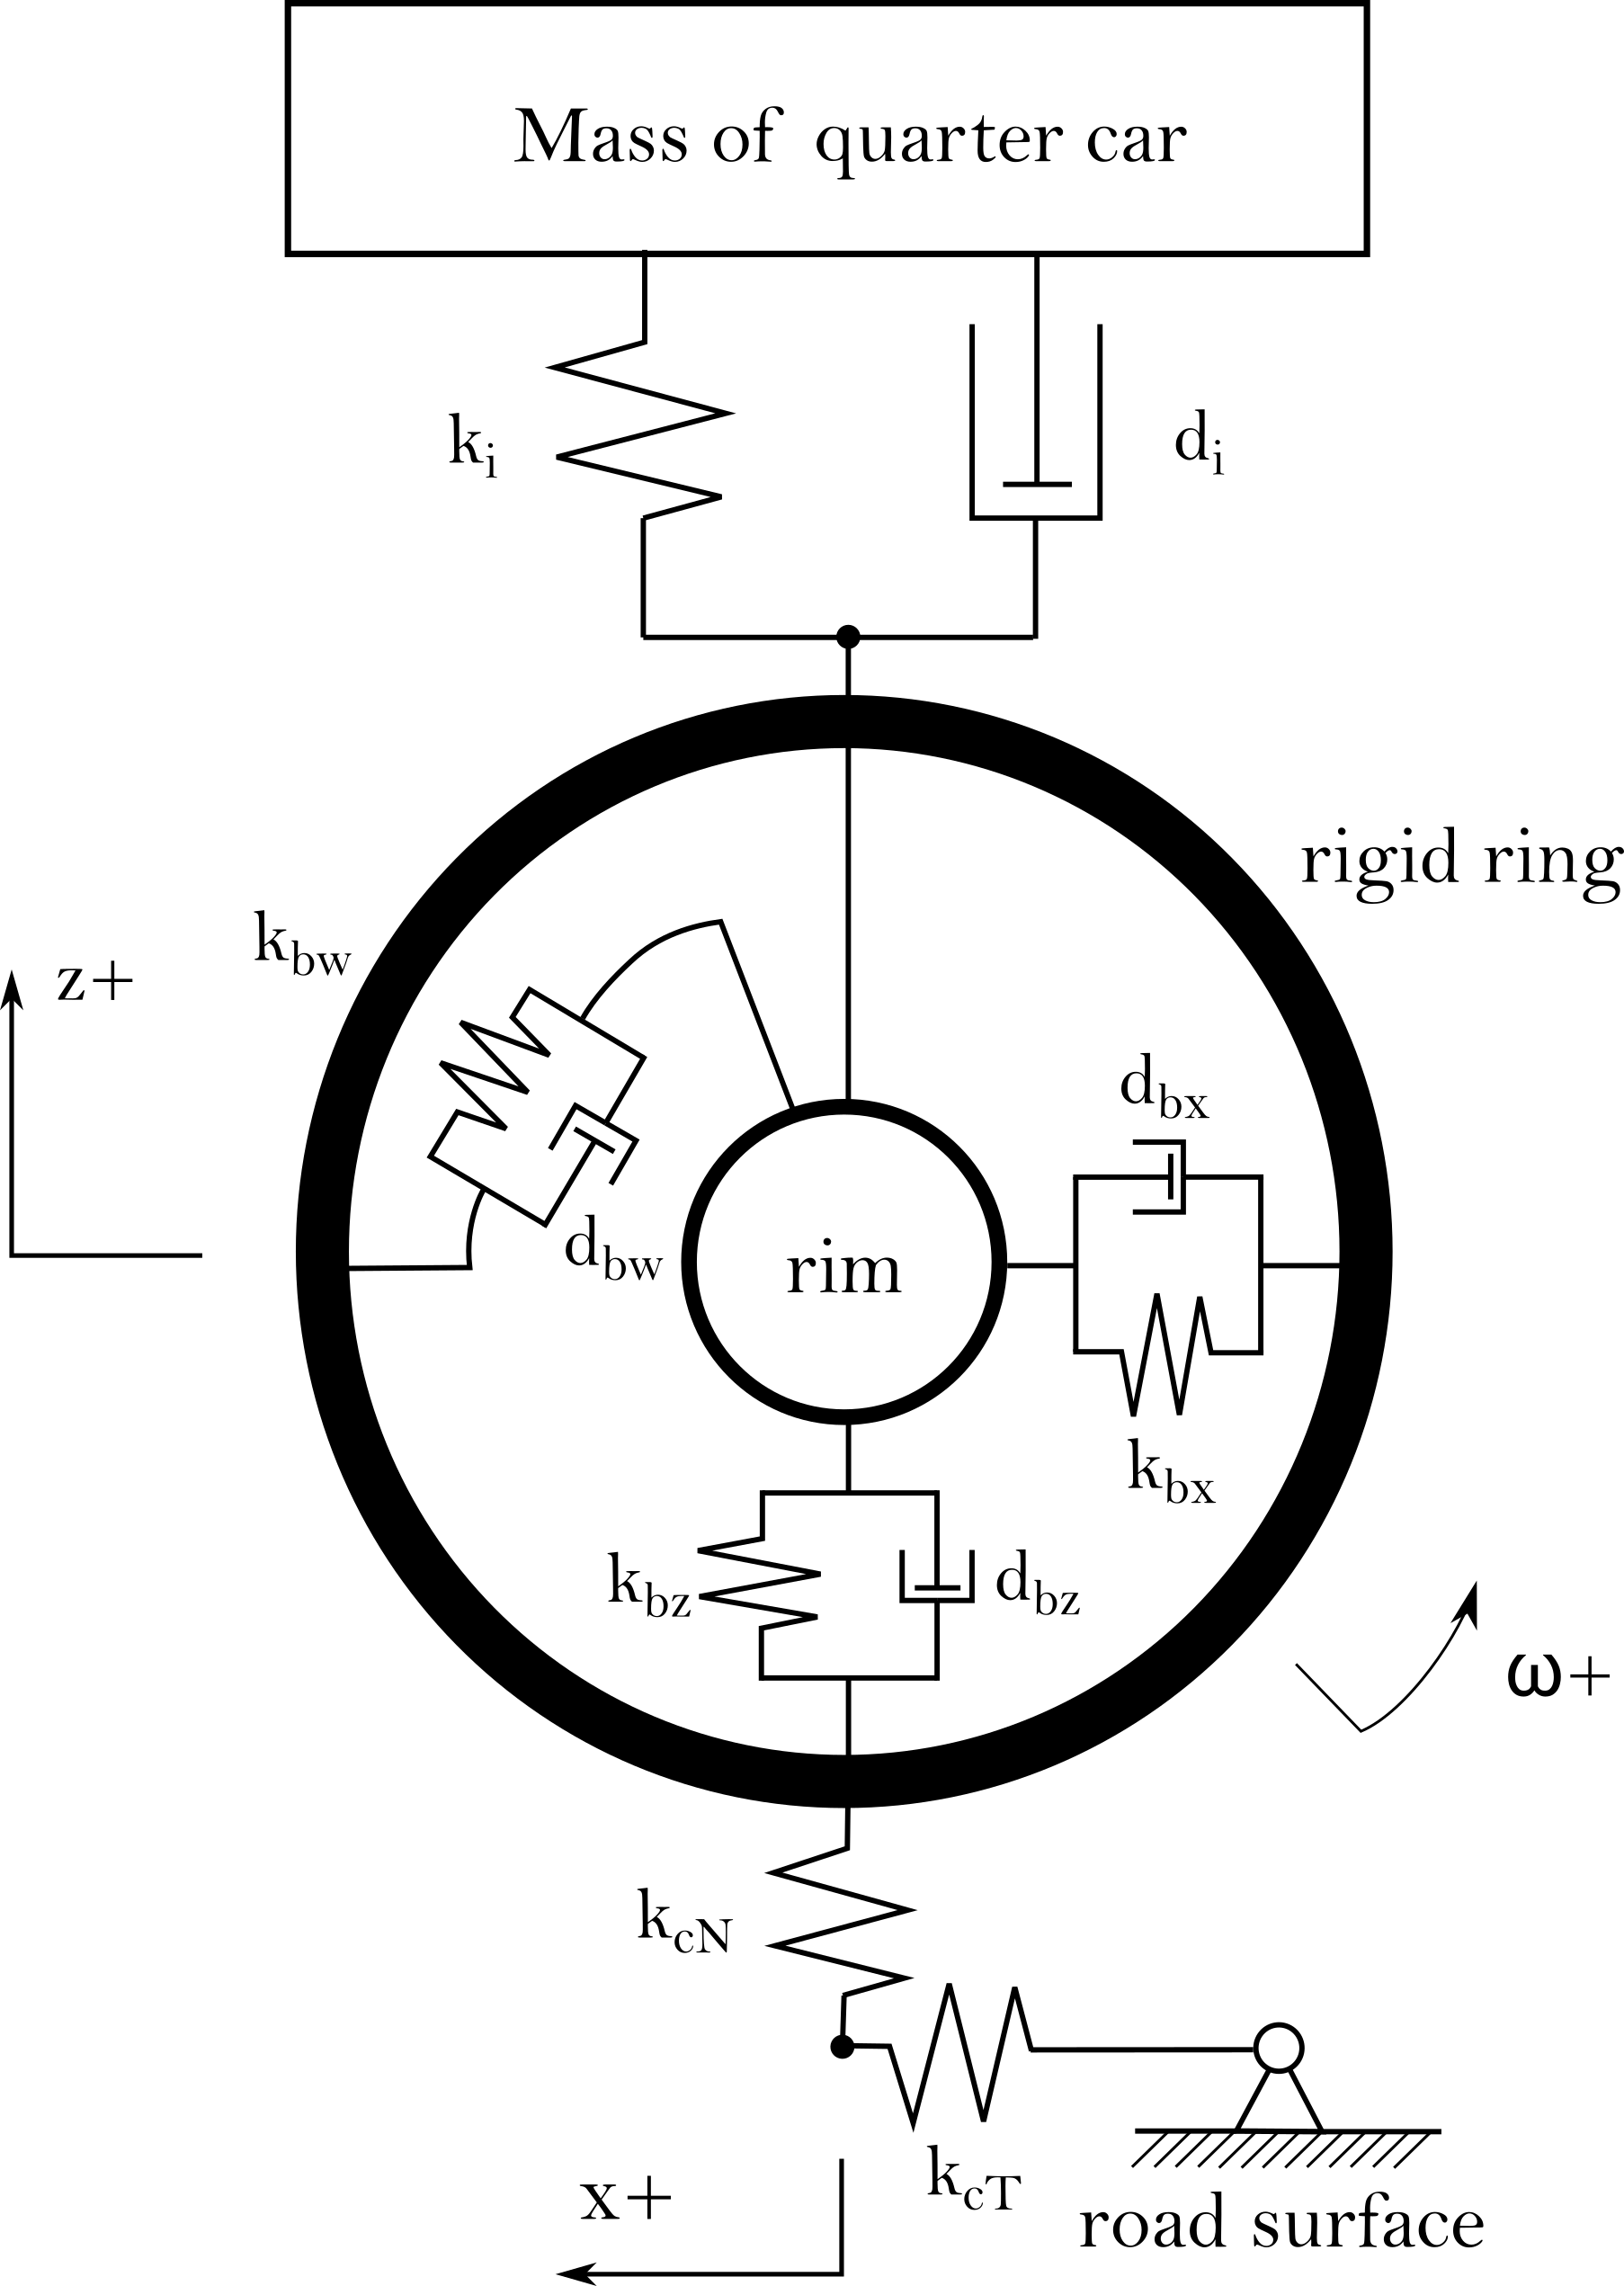
\includegraphics[width=0.4\textwidth]{bilder/rrm.png}
 \caption{Rigid ring model.}
 \label{fig:rrm}
 \end{figure}

The equations of motion for the rigid ring are

\begin{align}
\label{equ:rr}
m_b\ddot{x_b}+k_{bx}(x_b-x_r)+d_{bx}(\dot{x_b}-\dot{x_r}) &= cos\beta F_{cT}-sin\beta F_{cN} \\
m_b\ddot{z_b}+k_{bz}(z_b-z_r)+d_{bz}(\dot{z_b}-\dot{z_r}) &= -sin\beta F_{cT}-cos\beta F_{cN}\\
I_{by}\ddot{\omega_b}+k_{b\omega}(\omega_b-\omega_r)+d_{b\omega}(\dot{\omega_b}-\dot{\omega_r}) &=-r_eF_{ct}
\end{align}

where $k$ is the stiffness coefficient, $d$ is the damping coefficient, $F_{c}$ is the force from the contact patch, which $F_{cN}$ is the normal component and %F_{cT} is the tangential component.
%
$\omega$ is the effective road surface angle, and $r_e$ is the tire loaded radius.
%
The subscript 'r', 'b' and 'c' indicates the component rim, rigid ring and the contact patch).
%
The mass of the three components is denoted by $m$, the moment of inertia by $I_y$.

To implement the rigid ring tire model to the car model, we still need to build a force model for the $F_c$.
%
The normal force is the combination of the normal forces between the ground surface and the tread block due to the static quarter weight of the vehicle and the spring displacement and velocity damping between the ring and the tread block normal to the effective ground plane~\cite{na2016rigid}.
%
If the stiffness coefficient of the contact patch $k_cN$ and $k_cT$ are already known or can be measured.
%
The force $F_c$ is as

\begin{align}
\label{equ:contact_patch}
F_{cN} = k_{cN}(x_r-x_c)sin\beta+k_{cN}(z_r-z_c)cos\beta+Mg cos\beta \\
F_{cT} = k_{cT}(x_r-x_c)cos\beta+k_{cT}(z_r-z_c)sin\beta
\end{align}

If the stiffness coefficient of the contact patch is unknown or hard to measure.
%
\cite{zegelaar1998dynamic} introduces a way to describe the force of the contact patch, in which a residual deflection $\rho_{zr}$ is used to achieve a realistic overall tire stiffness.
%
The vertical force of the contact patch is resulted as

\begin{equation}
F_{cz} = q_{Fzr3}\rho_{zr}^3+q_{Fzr2}\rho^2+q_{Fzr1}\rho_{zr}+q_{V1}\Omega^2
\end{equation}

where $q$ indicate the coefficients set in~cite{} and $\Omega$ is the rim rotational velocity.
%
The residual deflection is as

\begin{equation}
\rho_{zr}=r-z_b+q_{V1}\Omega^2
\end{equation}

where $w$ is the effective road surface height.
%
The longitudinal force of the contace patch can be derived from the empirical Pacejka model.

\begin{equation}
F_{cx} = Asin(Barctan(Cs_x))
\end{equation}

where parameter $A,B,C$ have no direct physical meaing and are set from the system identification.
%
$s_l$ is the slip of the tire in the longitudinal direction and can be represented as

\begin{equation}
s_x=\frac{\dot{x_b}-r_e(\Omega+\dot{\theta_b})}{\dot{x_b}}
\end{equation}

Replacing the $m_ui$ as $m_r$ in the \ac{FCM} in Sec.~\ref{sec:active full car model}, then add the equation~\ref{equ:rr} of the rigid ring and the force model of the contact patch which is introduced in Equ.~\ref{equ:contact_patch} or in~cite{}, the rigid ring tire model is implemented in the \ac{FCM}.
%
It can be seen that in the rigid ring model the motion in the longitudinal direction is took into consideration, which is the advantage with the point contact tire model.
 
Besides, a more detailed and accuracy rigid ring model which is attended with a two or five point follower is introduced in \cite{na2016rigid}.
 
 
\subsection{Modified Point Contact Tire Model}
\label{sec:improved_pcm}
 
The rigid ring tire model is simple and efficient, but one additional consideration for developing the improved model is its suitability for using standard laboratory tests to measure the required lumped parameters for vertical, longitudinal, and torsional sidewall stiffness as well as tread, rigid ring, and bead/sidewall mass elements of four tires~\cite{na2016rigid}.

Cause the test laboratory is not available in the thesis, a modified point contact model is proposed to compromise the accuracy of the model and the financial situation.

The gain {$K$} is introduced to tune that is described as a function of the ratio {$e$} and the velocity of the vehicle {$v$}.


 \begin{equation}
 K=\begin{cases}
    a_0+a_1\cdot e^{a_2}\cdot v^{a_3} & (e < 1) \\
    1 & (e \geq 1)
 \end{cases}
 \end{equation}
 \label{form:K}
 
where

\begin{equation}
    e = \frac{l_{obstacle}}{l_{contact patch}}
\end{equation}

is the ratio between the length of obstacles and the tire contact patch.
%
$a_0, a_1, a_2, a_3$ are the factors of the description of the gain $K$.

When the tire crosses a obstacle, whose profile is below the road surface and its length is smaller than the tire contact patch, e.g a small and deep pothole or railway crossing, the height of the obstacle will be decreased in some degree by the gain.
%
The reason is that in this situation the real displacement of the wheel rim due to the elasticity of the rubber cannot be the same as the depth of the obstacles.

The situation is represented in Fig.~\ref{fig:tire}.
%
The real displacement of the wheel rim $\Delta z_u$ is smaller than the irregularity of the road profile $\Delta r$.
%
The less the ratio $e$ which represents a shorter obstacle wavelength, the slighter the influence from the obstacle on the displacement of the wheel rim.

 \begin{figure}
 \centering
 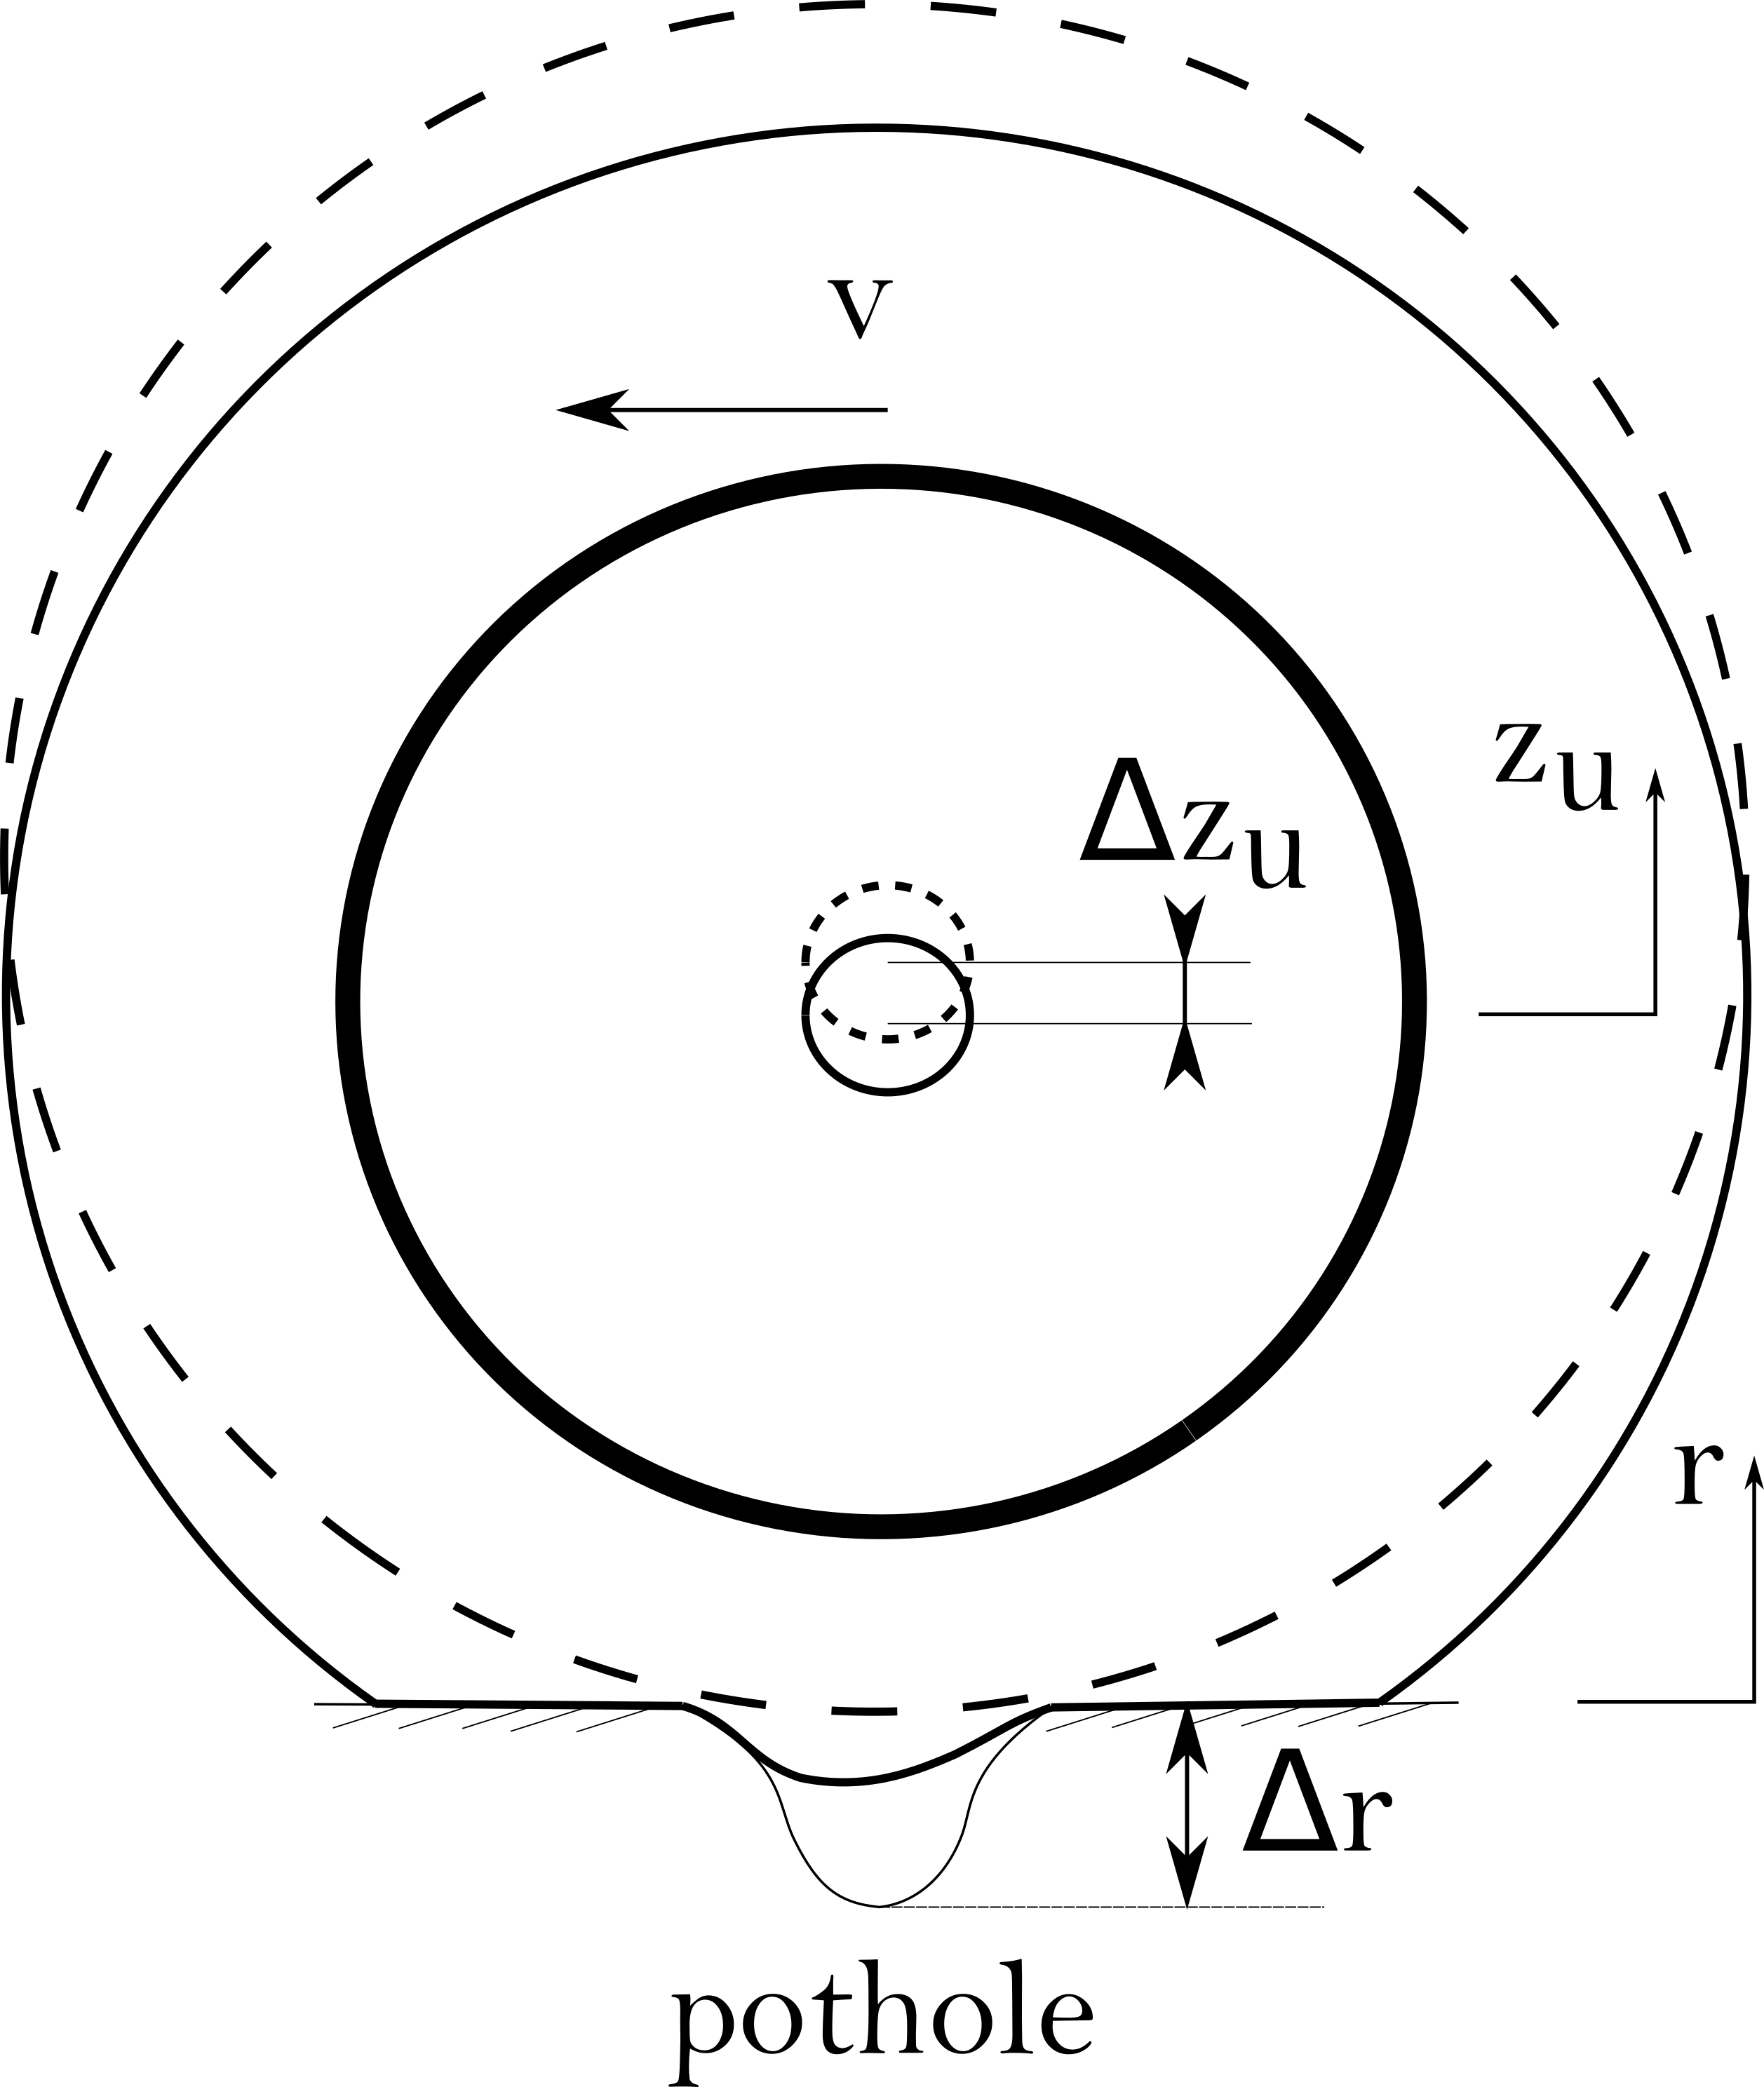
\includegraphics[width=0.3\textwidth]{bilder/tire.png}
 \caption{Contact situation with a short pothole.}
 \label{fig:tire}
 \end{figure}

While the tires crosses the obstacle whose profile is above the road surface and is steep, e.g a cleat or a step, the amplitude of the signal will be increased by $K$.
%
Except the vertical component of the velocity which will give an additional velocity to the wheel rim in vertical direction, the force that is generated during the crash by the obstacle has also a impact on the vehicle. 
%
The strength of the impact is related to the velocity of the vehicle.
%
The faster the velocity of the vehicle crosses the obstacle, the stronger the vibration is generated from the obstacle on the vehicle.

With this method the motion in the longitudinal direction and the interaction of the tire and the road have been considered in a simplified way.
%
The parameters {$a_0$}, {$a_1$}, {$a_2$}, {$a_3$} will be identified in Sections~\ref{sec:identification and validation}.	
	\chapter{Identification and validation}
 \label{sec:identification and validation}

 The model verification addresses the question whether the implemented model as a whole and its components conceptionally meet its criteria. 
 %
 According to the aim of the simulation that is to model the reality as perfect as possible, a real scenario in the simulation environment is exactly reproduced, including the elimination of errors in the model and the fine tuning of the parameters that were not available in the literature or through measurements. 
 %
 Considering the manufacturing and measurement tolerances, the model and the simulation will never be exactly the same. The claim for the simulation should thus be the qualitatively correct depiction of the trend shown by the real measurement. 
 
 Here the validation consist of two parts: Firstly, the identification of the damping coefficient and validation of the time response while traversing the speed bump with different velocities. Secondly, the identification of the parameters for formula~\ref{form:K} and validation of the vehicle vibration while traversing different obstacles with different velocities.
 %
 The real measurements are performed with a BMW 116d.
 
 
 \section{Identification and validation of the damping ratio}
 
 In one of the real measurements the vehicle drives at the speed of $20km/h$ across a speed bump which is $13mm$ high and $70mm$ wide on only one side of the road and the sensor is in the glove compartment (S4 in Sec.~\ref{sec:positionofoutput}). 
 %
 According to the principle of the validation, the situation should be identically reproduced in the simulation. 
 %
 The \ac{FCM} which will be used in the validation is with the basic point contact tire model because the parameter in \ref{form:K} is till unknown.
 %
 As what is mentioned in Sec.~\ref{sec:tire_model}, the point contact tire model performs good only when the wavelength of the obstacle greater than the contact patch, which is about $150mm$ long.
 
 Fig.~\ref{fig:tire_bump} shows the geometric relationship when the tire just meets the speed bump.
 %
 It can be seen that the tire has already touched the speed bump before the vehicle arrives the start point of it ($C$).
 %
 Hence in the simulation the start point of the speed bump should be at $D$, not $C$.
 %
 On the basis of the trigonometric function it is known that

 \begin{align}
    |AC|&=\sqrt{|AB|^2+|BC|^2}=\sqrt{13^2+(70/2)^2}mm = 37.4mm \\
    \angle A &= arctan(\frac{|BC|}{|AB|}) = \ang{70} \\
    \angle O_2&= \pi - 2*\angle A = \ang{40}
 \end{align}
 
 With the law of sines,
 \begin{equation}
    \frac{|AC|}{\angle O_2} = \frac{r_2}{\angle A}
 \end{equation} 
 
 Thus $r_2 = 53.6mm$.
 
 The radius of tire $r_1$ can be read from the sidewall of the tire. 
 %
 From the last dimension listed in the size number '195/55R16' it is known that the diameter of the wheel rim is 16 inch.
 %
 According to \cite{Tire_calculator} the diameter of the tire $r_1$ is about $660mm$.
 
 It is easy to calculate the length $|O_2D| \doteq 100mm$.
 %
 Hence the complete length of the speed bump in the simulation should be $2\cdot |O_2D| = 200mm$, which is greater than the contact patch.
 %
 It means the use of the basic point contact tire model is feasible in this situation.
 
 The speed bump is modeled by a sine function which is shown in Fig.~\ref{fig:bump}.
 %
 Addition to the roughness of the asphalt surface ($IRI=1$), the road model is created.
 %
 Tuning the damping ratio of the suspensions to get the results that is most similar to the actual measurement, including the peak of the amplitude and the duration of the vibration.
 
 \begin{figure}
 \centering
 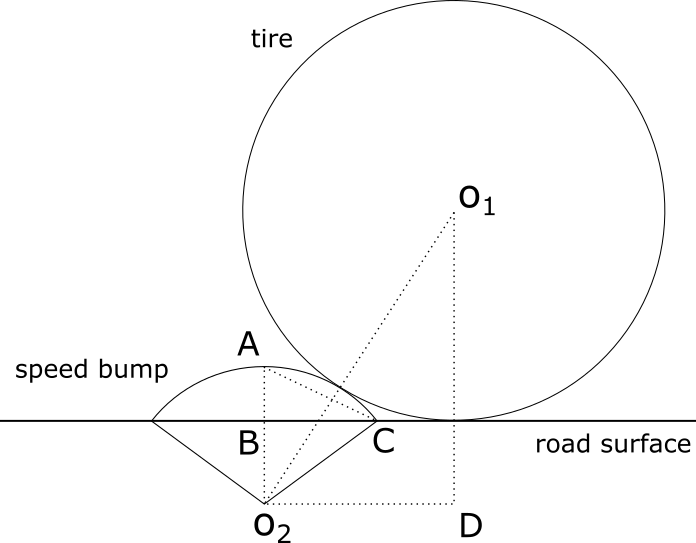
\includegraphics[width=0.5\textwidth]{bilder/validation.png}
 \caption{Geometric of the tire and speed bump.}
 \label{fig:tire_bump}
 \end{figure}
 
 
 
 \begin{figure}
 \centering
 \begin{tikzpicture}
 \begin{groupplot}[mygroupplot,
 group style={group name=my plots,group size= 1 by 1, horizontal sep=\myGroupSep,vertical sep=\myGroupVertSep},
 ]
 		
 	\nextgroupplot[
	ylabel= Height ($m$),
	xlabel= Length ($m$),
	%xmin=27,   
	%xmax=93,
   	ymin=0,   
   	%ymax=1.4,
% 	legend columns=1,
% 	legend entries={center of gravity, middle of left side},
% 	legend style={at={\myLegendPosition},anchor=south,name=leg},
    cycle list name=mycyclelist,
    ]
    \newcommand{\point}{1};
    \addplot+[no marks, each nth point=\point] table[x=r,y=h] {data/speed_bump.txt};
 
 \end{groupplot}
 \end{tikzpicture}
 \label{fig:bump}
 \caption{Profile of the simulated speed bump.}
 \end{figure}

 
 
 \begin{figure}
 \centering
 \begin{tikzpicture}
 \begin{groupplot}[mygroupplot,
 group style={group name=my plots,group size= 2 by 3, horizontal sep=\myGroupSep},
 ]
 		
 	\nextgroupplot[
	ylabel=Vertical acceleration ($g$),
	%xmin=27,   
	%xmax=93,
   	ymin=0.6,   
   	ymax=1.4,
% 	legend columns=1,
% 	legend entries={center of gravity, middle of left side},
% 	legend style={at={\myLegendPosition},anchor=south,name=leg},
    cycle list name=mycyclelist,
    ]
    \newcommand{\point}{1};
    \addplot+[no marks, each nth point=\point] table[x=x1,y=y3] {data/P3_20_Links3.txt};
    
    \nextgroupplot[
	%xmin=27,   
	%xmax=93,
   	ymin=0.6,   
   	ymax=1.4,
% 	legend columns=1,
% 	legend entries={center of gravity, middle of left side},
% 	legend style={at={\myLegendPosition},anchor=south,name=leg},
    cycle list name=mycyclelist,
    ]
    \newcommand{\point}{1};
    \addplot+[no marks, each nth point=\point] table[x=t,y=z] {data/validation_measure_data.txt};
    
    \nextgroupplot[
	%xlabel=Time ($s$),
	ylabel=Roll rate ($rad/s$),
	%xmin=27,   
	%xmax=93,
   	ymin=-0.04,   
  	ymax=0.06,
% 	legend columns=1,
% 	legend entries={center of gravity, middle of left side},
% 	legend style={at={\myLegendPosition},anchor=south,name=leg},
    cycle list name=mycyclelist,
    ]
    \newcommand{\point}{1};
    \addplot+[no marks, each nth point=\point] table[x=x1,y=y4] {data/P3_20_Links3.txt};
    
    \nextgroupplot[
	%xlabel=Time ($s$),
	%xmin=27,   
	%xmax=93,
    ymin=-0.04,   
  	ymax=0.06,
% 	legend columns=1,
% 	legend entries={center of gravity, middle of left side},
% 	legend style={at={\myLegendPosition},anchor=south,name=leg},
    cycle list name=mycyclelist,
    ]
    \newcommand{\point}{1};
    \addplot+[no marks, each nth point=\point] table[x=t,y=r] {data/validation_measure_data.txt};
    
    \nextgroupplot[
	xlabel=Time ($s$),
	ylabel=Pitch rate ($rad/s$),
	%xmin=27,   
	%xmax=93,
   	ymin=-0.04,   
  	ymax=0.04,
% 	legend columns=1,
% 	legend entries={center of gravity, middle of left side},
% 	legend style={at={\myLegendPosition},anchor=south,name=leg},
    cycle list name=mycyclelist,
    ]
    \newcommand{\point}{1};
    \addplot+[no marks, each nth point=\point] table[x=x1,y=y5] {data/P3_20_Links3.txt};
    
    \nextgroupplot[
	xlabel=Time ($s$),
	%xmin=27,   
	%xmax=93,
    ymin=-0.04,   
  	ymax=0.04,
% 	legend columns=1,
% 	legend entries={center of gravity, middle of left side},
% 	legend style={at={\myLegendPosition},anchor=south,name=leg},
    cycle list name=mycyclelist,
    ]
    \newcommand{\point}{1};
    \addplot+[no marks, each nth point=\point] table[x=t,y=p] {data/validation_measure_p.txt};
 
 \end{groupplot}
 
 \node[below = \myLabelSep of my plots c1r3.south] {(a) real measurements};
 \node[below = \myLabelSep of my plots c2r3.south] {(b) simulation};
 
 \end{tikzpicture}
 \label{fig:validation_bump}
 \caption{Comparison of the vehicle response to a speed bump.}
 \end{figure}
 

The identified coefficient of the damping is shown in table~\ref{tbl:damping}.
%
With those coefficient the comparison between the measured data and the simulation is shown in Fig.~\ref{fig:validation_bump}.
% 
It can be seen that although the value of the peaks do not complete match the reality, the general behaviour of the simulation is very similar to the actual measurement, which validates that the \ac{FCM} can correctly simulate the behaviour of a real vehicle.

\begin{table}
\centering
\caption{Stiffness and damping ratio of the full car model.}
\label{tbl:damping}
\begin{tabular}{lcccccccc}
\hline
variable & $k_1$ & $k_2$ & $k_3$ & $k_4$ & $d_1$ & $d_2$ & $d_3$ & $d_4$ \\
unit & \multicolumn{4}{c}{$[kN\cdot m^{-1}]$} & \multicolumn{4}{c}{[$kN\cdot s \cdot m^{-1}]$} \\
value & 16 & 16 & 16 & 16 & 1 & 1 & 1 & 1 \\ \hline
\end{tabular}
\end{table}
 
 
 
 
 
 
 \section{Identification and validation of the tire model}
 
 
 \begin{table}
 \centering
 \caption{Parameters for $K$ and size of different events.}
 \label{tbl:parameter of K}
 \begin{tabular}{lllllll}
 \hline
 events & $a_0$ & $a_1$ & $a_2$ & $a_3$ & $l/[m]$ & $h/[m]$ \\ \hline
 pothole & 0 & 0.03 & 1 & 1 & 0.5 & 0.02\\
 manhole cover & 0 & 0.015 & 0 & 1 & 0.5 & 0.01 \\
 cobbled road & 0 & 0.04 & 1 & 1 & 0.2 & 0.02 \\
 railway crossing & 0.02 & 0 & 0 & 0 & 1.45 & 0.1\\ \hline
 \end{tabular}
 \end{table}
 
 
 \begin{figure}
 \centering
 \begin{tikzpicture}
 \begin{groupplot}[mygroupplot,
 group style={group name=my plots,group size= 2 by 3, horizontal sep=\myGroupSep,vertical sep=\myGroupVertSep}]
 		
 	\nextgroupplot[
	ylabel=$\sigma$(vertical acceleration) ($m/s^2$),
	%xmin=27,   
	%xmax=93,
   	ymin=0,   
   	ymax=0.4,
   	cycle list name=mycyclelist,
    ]
    \newcommand{\point}{1};
    \addplot+[error bars/.cd, y dir=both,y explicit]
    coordinates {
    (8.3,0.027) +- (0.00085,0.00085)
    (11.1,0.036) +- (0.009,0.009)
    (13.9,0.0396) +- (0.0007,0.0007)
    (16.7,0.0476) +- (0.0012,0.0012)};
    %\addlegendentry{Asphalt}
    
    \addplot+[error bars/.cd, y dir=both,y explicit]
    coordinates {
    (8.3,0.04) +- (0.0005,0.0005)
    (11.1,0.046) +- (0.0037,0.00037)
    (13.9,0.048) +- (0.0035,0.0035)
    (16.7,0.05) +- (0.0041,0.0041)};
    %\addlegendentry{Railroad crossing}
    
    \addplot+[error bars/.cd, y dir=both,y explicit]
    coordinates {
    (8.3,0.045) +- (0.0034,0.0034)
    (11.1,0.059) +- (0.0036,0.0036)
    (13.9,0.074) +- (0.003,0.003)
    (16.7,0.1) +- (0.0028,0.0028)};
   % \addlegendentry{Manhole cover}

    \addplot+[error bars/.cd, y dir=both,y explicit]
    coordinates {
    (8.3,0.129) +- (0.0039,0.0039)
    (11.1,0.161) +- (0.0029,0.0029)
    (13.9,0.168) +- (0.001,0.001)
    (16.7,0.177) +- (0.0015,0.0015)};
    %\addlegendentry{Cobbled road}

    \addplot+[error bars/.cd, y dir=both,y explicit]
    coordinates {
    (8.3,0.18) +- (0.0072,0.0072)
    (11.1,0.28) +- (0.014,0.014)
    (13.9,0.3) +- (0.025,0.025)
    (16.7,0.3) +- (0.012,0.012)};
   % \addlegendentry{Pothole}

    \addplot+[error bars/.cd, y dir=both,y explicit]
    coordinates {
    (8.3,0.116) +- (0.0041,0.0041)
    (11.1,0.142) +- (0.0017,0.0017)
    (13.9,0.164) +- (0.0023,0.0023)
    (16.7,0.184) +- (0.002,0.002)};
    %\addlegendentry{Unevennesses}
    
    \nextgroupplot[
	%ylabel=$\sigma$(vertical acceleration) ($m/s^2$),
	%xmin=27,   
	%xmax=93,
   	ymin=0,   
   	ymax=0.4,
   	legend columns=3,
  	legend style={at={(-0.3,1.03)},anchor=south,name=leg},
  	cycle list name=mycyclelist,
    ]
    \newcommand{\point}{1};
    \addplot+[error bars/.cd, y dir=both,y explicit]
    table[x = v, y = m1, y error = e1]{data/ddz_obstacles_velocity.txt};
    \addlegendentry{asphalt}
    
    \addplot+[error bars/.cd, y dir=both,y explicit]
    table[x = v, y = m2, y error = e2]{data/ddz_obstacles_velocity.txt};
    \addlegendentry{railroad crossing}
    
    \addplot+[error bars/.cd, y dir=both,y explicit]
    table[x = v, y = m3, y error = e3]{data/ddz_obstacles_velocity.txt};
    \addlegendentry{manhole cover}

    \addplot+[error bars/.cd, y dir=both,y explicit]
    table[x = v, y = m4, y error = e4]{data/ddz_obstacles_velocity.txt};
   \addlegendentry{cobbled road}

    \addplot+[error bars/.cd, y dir=both,y explicit]
    table[x = v, y = m5, y error = e5]{data/ddz_obstacles_velocity.txt};
   \addlegendentry{pothole}

    \addplot+[error bars/.cd, y dir=both,y explicit]
    table[x = v, y = m6, y error = e6]{data/ddz_obstacles_velocity.txt};
   \addlegendentry{unevenness}
    
    \nextgroupplot[
	%xlabel=Velocity ($m/s$),
	ylabel=$\sigma$(roll rate) ($rad/s$),
	%xmin=27,   
	%xmax=93,
   	ymin=0,   
   	ymax=0.05,
% 	legend columns=1,
% 	legend entries={center of gravity, middle of left side},
% 	legend style={at={\myLegendPosition},anchor=south,name=leg},
    cycle list name=mycyclelist,
    ]
    \newcommand{\point}{1};
    \addplot+[error bars/.cd, y dir=both,y explicit]
    coordinates {
	(8.3,0.0034) +- (0.00014,0.00014)
	(11.1,0.0040) +- (0.000082,0.000082)
	(13.9,0.00453) +- (0.000062,0.000062)
	(16.7,0.0061) +- (0.00027,0.00027)};
	%\addlegendentry{Asphalt}
 
    \addplot+[error bars/.cd, y dir=both,y explicit]
    coordinates {
    (8.3,0.0081) +- (0.0006,0.0006)
    (11.1,0.0088) +- (0.00027,0.00027)
    (13.9,0.008) +- (0.00055,0.00055)
    (16.7,0.0088) +- (0.00044,0.00044)};
    %\addlegendentry{Railroad crossing}
    
    \addplot+[error bars/.cd, y dir=both,y explicit]
    coordinates {
    (8.3,0.00945) +- (0.00027,0.00027)
    (11.1,0.0139) +- (0.00064,0.00064)
    (13.9,0.015) +- (0.0011,0.0011)
	(16.7,0.028) +- (0.00028,0.00028)};
	%\addlegendentry{Manhole cover}
	
	\addplot+[error bars/.cd, y dir=both,y explicit]
	coordinates {
	(8.3,0.0192) +- (0.0003,0.0003)
	(11.1,0.024) +- (0.00045,0.00045)
	(13.9,0.0275) +- (0.00022,0.00022)
	(16.7,0.0299) +- (0.00033,0.00033)};
	%\addlegendentry{Cobbled road}
	
	\addplot+[error bars/.cd, y dir=both,y explicit]
	coordinates {
	(8.3,0.0288) +- (0.00045,0.00045)
	(11.1,0.036) +- (0.0011,0.0011)
	(13.9,0.046) +- (0.0008,0.0008)
	(16.7,0.04) +- (0.0002,0.0002)};
	%\addlegendentry{Pothole}
	
	\addplot+[error bars/.cd, y dir=both,y explicit]
	coordinates {
	(8.3,0.0187) +- (0.00012,0.00012)
	(11.1,0.0224) +- (0.0004,0.0004)
	(13.9,0.0245) +- (0.00027,0.00027)
	(16.7,0.027) +- (0.0005,0.0005)};
	%\addlegendentry{Unevennesses}
	
	\nextgroupplot[
	%xlabel=Velocity ($m/s$),
	%ylabel=$\sigma$(roll rate) ($rad/s$),
	%xmin=27,   
	%xmax=93,
   	ymin=0,   
   	ymax=0.05,
% 	legend columns=1,
% 	legend entries={center of gravity, middle of left side},
% 	legend style={at={\myLegendPosition},anchor=south,name=leg},
    cycle list name=mycyclelist,
    ]
    \newcommand{\point}{1};
    \addplot+[error bars/.cd, y dir=both,y explicit]
    table[x = v, y = m1, y error = e1]{data/ddr_obstacles_velocity.txt};
    %\addlegendentry{Asphalt}
    
    \addplot+[error bars/.cd, y dir=both,y explicit]
    table[x = v, y = m2, y error = e2]{data/ddr_obstacles_velocity.txt};
    %\addlegendentry{Railroad crossing}
    
    \addplot+[error bars/.cd, y dir=both,y explicit]
    table[x = v, y = m3, y error = e3]{data/ddr_obstacles_velocity.txt};
    %\addlegendentry{Manhole cover}

    \addplot+[error bars/.cd, y dir=both,y explicit]
    table[x = v, y = m4, y error = e4]{data/ddr_obstacles_velocity.txt};
    %\addlegendentry{Cobbled road}

    \addplot+[error bars/.cd, y dir=both,y explicit]
    table[x = v, y = m5, y error = e5]{data/ddr_obstacles_velocity.txt};
    %\addlegendentry{Pothole}

    \addplot+[error bars/.cd, y dir=both,y explicit]
    table[x = v, y = m6, y error = e6]{data/ddr_obstacles_velocity.txt};
    %\addlegendentry{Unevennesses}
    
    
     \nextgroupplot[
	xlabel=Velocity ($m/s$),
	ylabel=$\sigma$(pitch rate) ($rad/s$),
	%xmin=27,   
	%xmax=93,
   	ymin=0,   
   	ymax=0.07,
% 	legend columns=1,
% 	legend entries={center of gravity, middle of left side},
% 	legend style={at={\myLegendPosition},anchor=south,name=leg},
    cycle list name=mycyclelist,
    ]
    \newcommand{\point}{1};
    \addplot+[error bars/.cd, y dir=both,y explicit]
    coordinates {
	(8.3,0.0064) +- (0.00003,0.00003)
	(11.1,0.00675) +- (0.0001,0.0001)
	(13.9,0.008) +- (0.0002,0.0002)
	(16.7,0.0097) +- (0.0001,0.0001)};
	%\addlegendentry{Asphalt}
 
    \addplot+[error bars/.cd, y dir=both,y explicit]
    coordinates {
    (8.3,0.011) +- (0.00035,0.00035)
	(11.1,0.0129) +- (0.00039,0.00039)
	(13.9,0.0125) +- (0.00052,0.00052)
	(16.7,0.0113) +- (0.0013,0.0013)};
    %\addlegendentry{Railroad crossing}
    
    \addplot+[error bars/.cd, y dir=both,y explicit]
    coordinates {
    (8.3,0.0167) +- (0.00096,0.00096)
	(11.1,0.0176) +- (0.00021,0.00021)
	(13.9,0.022) +- (0.001,0.001)
	(16.7,0.034) +- (0.001,0.001)};
	%\addlegendentry{Manhole cover}
	
	\addplot+[error bars/.cd, y dir=both,y explicit]
	coordinates {
	(8.3,0.0326) +- (0.0002,0.0002)
	(11.1,0.0355) +- (0.00023,0.00023)
	(13.9,0.0371) +- (0.0003,0.0003)
	(16.7,0.0382) +- (0.00012,0.00012)};
	%\addlegendentry{Cobbled road}
	
	\addplot+[error bars/.cd, y dir=both,y explicit]
	coordinates {
	(8.3,0.051) +- (0.0016,0.0016)
	(11.1,0.061) +- (0.0018,0.0018)
	(13.9,0.065) +- (0.004,0.004)
	(16.7,0.063) +- (0.001,0.001)};
	%\addlegendentry{Pothole}
	
	\addplot+[error bars/.cd, y dir=both,y explicit]
	coordinates {
	(8.3,0.0291) +- (0.00023,0.00023)
	(11.1,0.033) +- (0.0003,0.0003)
	(13.9,0.0373) +- (0.0005,0.0005)
	(16.7,0.041) +- (0.00028,0.00028)};
	%\addlegendentry{Unevennesses}
	
	\nextgroupplot[
	xlabel=Velocity ($m/s$),
	%ylabel=$\sigma$(roll rate) ($rad/s$),
	%xmin=27,   
	%xmax=93,
   	ymin=0,   
   	ymax=0.07,
% 	legend columns=1,
% 	legend entries={center of gravity, middle of left side},
% 	legend style={at={\myLegendPosition},anchor=south,name=leg},
    cycle list name=mycyclelist,
    ]
    \newcommand{\point}{1};
    \addplot+[error bars/.cd, y dir=both,y explicit]
    table[x = v, y = m1, y error = e1]{data/ddp_obstacles_velocity.txt};
    %\addlegendentry{Asphalt}
    
    \addplot+[error bars/.cd, y dir=both,y explicit]
    table[x = v, y = m2, y error = e2]{data/ddp_obstacles_velocity.txt};
    %\addlegendentry{Railroad crossing}
    
    \addplot+[error bars/.cd, y dir=both,y explicit]
    table[x = v, y = m3, y error = e3]{data/ddp_obstacles_velocity.txt};
    %\addlegendentry{Manhole cover}

    \addplot+[error bars/.cd, y dir=both,y explicit]
    table[x = v, y = m4, y error = e4]{data/ddp_obstacles_velocity.txt};
    %\addlegendentry{Cobbled road}

    \addplot+[error bars/.cd, y dir=both,y explicit]
    table[x = v, y = m5, y error = e5]{data/ddp_obstacles_velocity.txt};
    %\addlegendentry{Pothole}

    \addplot+[error bars/.cd, y dir=both,y explicit]
    table[x = v, y = m6, y error = e6]{data/ddp_obstacles_velocity.txt};
    %\addlegendentry{Unevennesses}
 
 \end{groupplot}
 
\node[below = \myLabelSep of my plots c1r3.south] {(a) real measurements};
\node[below = \myLabelSep of my plots c2r3.south] {(b) simulation};
 
 \end{tikzpicture}
 \label{fig:validation_events}
 \caption{Comparison of the standard deviation $\sigma$ of vertical acceleration, roll rate and pitch rate between real measurement and simulated results.}
 \end{figure}
 
 
 
 To identify the parameter in the formula~\ref{form:K}, different obstacles with different wavelength should be tested.
 %
 In the real driving test the the BMW 116d crosses six different events including asphalt road, pothole, manhole cover, railway crossing, cobbled road and evenness at four different velocities form $20km/h$ to $60km/h$
 
 All of the following outputs are measured at the center of gravity. 
 %
 For each velocity and each measuring event four runs are conducted and then the averaged value of the parameter is reported.
 %
 The error bars show the standard deviation of the obtained values.
 
 The best situation is that the modified point contact model can be applied in all different obstacles after the identification.
 %
 However, it hard to fulfill due to the simply structure an principle of the model.
 %
 The dynamic process between the obstacle and tire is so complicated that it is difficult to build a accuracy model with the point contact model an only two variables $e$ and $v$.
 
 Thus, for different obstacles different parameters of formula~\ref{form:K} should be identified separately to describe the real motion of the tire and the road.
 %
 Although the amount of the labor has increased, the results proves to be satisfied. 
 %
 The result of the measured data and the simulation after the identification are shown in Fig.~\ref{fig:validation_events}.
 %
 And the identified parameters of the filer are shown in table~\ref{tbl:parameter of K}. 
 
 It is observed that the simulated results have a very similar distribution as the measured data. 
 %
 Despite some simulated value has a deviation from the real data, the tendency and the relative position of different outputs by different obstacles are in general the same as the results of the measurement.
 %
 These clearly and correctly divided data has a positive influence on the accuracy of the classification.
 
 After the vehicle model and road model have been appropriately identified, the outputs provides not only a generally accuracy of the value e.g. the vertical acceleration, roll rate and pitch rate, also performs a similar features and relations compared with the actual data e.g. the duration of the signal and the standard deviations of different signals.
 
 In conclusion, the data which has been simulated by the road- and vehicle model is proved to be in the line with the facts.
 %
 Thus, the results and accuracy of the data processing in the next chapters shall be reasonable and well-founded.
 
 
 	
	\chapter{Methodology}

\section{Data processing}

\begin{figure}
\centering
\footnotesize
\begin{tikzpicture}[node distance = 2cm]

\tikzstyle{block} = [rectangle, draw, text width=10em, text centered, rounded corners, minimum height=4em]
\tikzstyle{line} = [draw, -latex']
\tikzstyle{cloud} = [draw, ellipse, minimum height=3em,text width=5em, text centered]
\tikzstyle{do} = [draw, dashed, ellipse, minimum height=3em, minimum width=6em, text centered]


\node [cloud] (sensor) {Data};
\node [block, below= of sensor] (extract) {Feature extraction};
\node [block, below= of extract] (selection) {Feature selection};
\node [block, below= of selection] (aggregation) {Feature aggregation};
\node [block, below= of aggregation] (classification) {Classification};
\node [cloud, below= of classification] (output) {Output};

\node [do, above right = 2em and 2em of classification, node distance=1.5cm] (testing) {Training};
\node [do, below right = 2em and 2em of classification, node distance=1.5cm] (training) {Testing};

    
\path [line] (sensor) -- node [left] {Vehicle dynamic} node [right] {matrix} (extract);

\path [line] (extract) -- node[left] {$n$-dimension features} node[right] {vector} (selection);

\path [line] (selection) -- node [left, fill=white] {$\tilde{n}$-dimension features} node [right, fill=white] {vector ($\tilde{n} \leq n$)} (aggregation);

\path [line] (aggregation) -- node[left] {$\mathring{n} $-dimension features} node[right] {vect. ($\mathring{n} \leq \tilde{n})$} (classification);

\path [line] (classification) -- node[left] {Class $K_i$} node[right] {$i=1,...,k$} (output);  
 

 \path [line,dashed] (training) -- (classification);
 \path [line,dashed] (testing) -- (classification);

\end{tikzpicture}

\caption{Overview of the method to predict road features of class $K_i$ based on vehicle dynamic data from simulation.}%
\label{fig:flowchart}%
\end{figure}

The goal is to find a function $f_X$, which classifies the road infrastructure, e.g. the road condition, based on the vehicle dynamic data from the simulation.
%
A supervised learning approach and a \ac{SVM} is used to find such a function.
%
\ac{SVM} is a supervised learning technique that can only be used for classification and regression
tasks.
%
The biggest advantage of a \ac{SVM} is that it is the only technique that is explicitly based on
learning theory.
%
Other techniques like neuronal networks and decision trees have local minima as problems, which the SVM does not have, as it always tries to separate the data points with maximum margin and hence always finds the global minimum.
%
A basic \ac{SVM} is a binary, linear classifier, meaning it can only distinguish between two different classes that are linearly separable.
%
For the use in problems that can not be separated with a straight line, the kernel-trick is applied to map the data points in a higher dimensional space where they can again be separated by a line.

It is often used for problems with a high number of features, as its performance is not affected by the number of features.
%
Features are extracted from the raw data to reduce the dimension and to characterize the vehicle response due to various road obstacles and builds derived values intended to be informative and non-redundant.
%
Besides, each feature set must be labeled with the ground truth data, otherwise the features are meaningless.

Determining a subset of the initial features is called feature selection.
%
The selected features are expected to contain the relevant information from the input data, so that the desired task can be performed by using this reduced representation instead of the complete initial data \cite{alpaydin2014introduction}.
%
The central premise when using a feature selection technique is that the data contains many features that are either redundant or irrelevant, and can thus be removed without incurring much loss of information~\cite{bermingham2015application}.
%
Redundant or irrelevant features are two distinct notions, since one relevant feature may be redundant in the presence of another relevant feature with which it is strongly correlated.
This results in a $n$-dimensional feature vector, which dimension can be reduced with feature selection and feature aggregation~\cite{guyon2003introduction}.
%
With statistical methods, redundant or irrelevant features can be eliminated, which enhances the generalization and avoids over-fitting.
%
In this thesis \ac{MANOVA} is used to select the best features.

The dimension of the feature vector can be further reduced through feature aggregation.
%
For this purpose \ac{LDA} is applied.
%
After the classifier is trained, the model can be tested with new labeled data.
%
Figure~\ref{fig:flowchart} summarizes the methods to process the vehicle dynamic data.

From the correct and false predicted instances, we can calculate a confusion matrix $M=(m_{ij})\in \mathbb{N}^{k \times k}$ for classes $K_i, i=1,\dotsc,k$.
%
In the confusion matrix, $m_{ii}$ presents the \textit{true positives} for class $i$. 
%
The other elements in column $j$ are called \textit{false negatives}, in row $i$ \textit{false positives} and in the diagonal \textit{true negatives}. 

From the confusion matrix, one can calculate multiple performance measures to evaluate the model, such as recall with $\frac{m_{ii}}{\sum_{j=1}^n{m_{ji}}}$ for class $K_i$, the overall accuracy of the classifier with $\frac{\sum_{i=1}^n{m_{ii}}}{\sum_{i=1}^n\sum_{j=1}^n{m_{ij}}}$, or the precision $\frac{m_{ij}}{\sum_{j=1}^n{m_{ij}}} = \pi_{ij}$. 
%
The precision presents the fraction of retrieved instances that are relevant and can be seen as the probability $\pi_{ij}$ of the classifier to predict class $i$ as class $j$ for $i,j=1,\dotsc,l$.
%
An overview for performance measures for different calculation problems can be found in \cite{Sokolova2009427}.
%
The data is processed with the \textsc{SciXMiner} toolbox for \textsc{Matlab}~\cite{mikut2017matlab}.




 
 \section{Road events and data labelling}
 
 The Data which is used for the training and testing for the classifier is simulated by the different road model and vehicle model which is introduced in chapter \ref{chaptr:simulation}.
 %
 There are six classes of the events including asphalt road, pothole, manhole cover, railway crossing and unevenness road used in the simulation.
 %
 Each of the events represents a type of obstacle is labeled from 1 to 6 as the output variables for the classification of training and as the ground truths in the process of testing.
 %
 The length and height of the events can be randomly varied from 0.5 to 2.5 times over the road profile.
 %
 This road model is described in Sec.~\ref{sec:roadmodel}.
 %
 For training and testing several road profiles with multiple road events are created as the input variables of the simulation.
 %
 Particularly, the profiles of the road model for testing are randomly created to investigate the robustness of the classifier which is trained by a fixed road model with a amount of variations.





 
 \section{Feature extraction}
 \label{sec:feature_ex}

 With the road model as the input of the full car model we can get the response outputs including vertical acceleration, roll acceleration and pitch acceleration of the vehicle body in time or space domain. 
 %
 The advantage of the space domain over the time domain is that every event is located at the same spot no matter how fast the car is driving, which makes it convenient and efficient to divide the windows of the data.
 %
 Furthermore, the vehicle vibration is dependent on the velocity, which can be minimized by transforming the time series data into space series data \cite{ward_speed-independent_2009}.

 The features should carry the representative information of the current road segment and be able to distinguish the difference of the response of each event.
 %
 All the 98 extracted features are calculated in a certain window length of $5m$ and overlap $50\%$ from the whole response outputs. 
 %
 The features include the mean velocity of the vehicle; maximum, minimum and mean value of the signals; range between the maximum and minimum; duration between the two extreme, \ac{RMS} which is defined as the square root of the mean square, and \ac{Std}.
 %
 These features can reflect the character of the data in the space domain.
 
 As well as \ac{intBP} from $1Hz$ to $30Hz$ with the interval $2Hz$ which indicates the weight of the selected frequency in all the pass band, \ac{maxBP} from $1Hz$ to $30Hz$ with the interval $2Hz$ which indicates the maximum magnitude of the selected frequency, \ac{PSD} which describes the distribution of power into frequency components, and the spectral centroid which indicates where the ’center of mass’ of the spectrum is and hence represents the the most common frequency in this window.
 %
 These features can reflect the character of the data in the frequency domain.
 


\section{Display and evaluation of the classification}
\label{sec:evaluation}
 
The results will be evaluated in this chapter by the confusion matrix and graphics.
%
In the display of the graphic the axles represent the selected features, the color of the point cloud represents different events.
%
The clouds may be overlapped or separated, which represent the performance of the classifier with those selected features.

In the confusion matrix each class has one row and one column in this matrix and they are arranged in the same order.
%
The rows represent the actual class membership and columns represent the predicted class.
%
This means that all correctly classified data points are the diagonal elements of the matrix.
%
While other points are classified false.
%
An example of a confusion matrix is presented in table \ref{tbl:confusion_matrix}.

\begin{table}[]
\centering
\caption{Example of a confusion matrix}
\label{tbl:confusion_matrix}
\begin{tabular}{cccc}
\hline
 & \multicolumn{3}{c}{Prediction} \\ \hline
 &  & + & - \\
Actual class & + & true positive & false negative \\
 & - & false positive & true negative \\ \hline
\end{tabular}
\end{table}

There are three performance measures to get meaningful information from the confusion matrix.
%
The first measure is 'Precision'.
%
This measure represents for each class the percentage of correctly classified members of this class among all points that were predicted as members of this class by the classifier.
%
Take the confusion matrix \ref{tbl:confusion_matrix} as the example of calculation

\begin{equation}
    Precision_{+} = \frac{\Sigma true~Positives}{\Sigma predicted~condition~positive}
\end{equation}

The second measure is 'Recall'.
%
It represents for each class the percentage of correctly classified members of this class among all actual members of this class.

\begin{equation}
    Recall_{+} = \frac{\Sigma true~positives}{\Sigma total~number~of~actual~Positives}
\end{equation}

The last measure is 'Accuracy'.
%
It is a general evaluation of the performance of a classifier.

\begin{equation}
    Accuracy = \frac{\Sigma true~positives + \Sigma true~negatives}{\Sigma total~number~of~data~point}
\end{equation}

From these performance measures it can be seen whether the classifier performs good for all classes or only several classes.

In supervised learning applications in machine learning and statistical learning theory, generalization error is a measure of how accurately an algorithm is able to predict outcome values for previously unseen data.
%
Because learning algorithms are evaluated on finite samples, the evaluation of a learning algorithm may be sensitive to sampling error.
%
As a result, measurements of prediction error on the current data may not provide much information about predictive ability on new data.
 
The generalization error $G$ is the difference between the expected error $I[f_n]$ and empirical error $I_S[f_n]$.
 
 \begin{equation}
    G=I[f_n]-I_S[f_n]
 \end{equation}
 
 Generalization error can be minimized by avoiding overfitting or overtraining in the learning algorithm.
 %
 In general, this error should shrink with the amount of training data before the testing.
 
 
 
 
 \section{Variation of simulation}
 
 There are many parameters influencing the classification process.
 %
 Regarding the variation of the vehicles, the model and physical parameters of the vehicle, the type of suspension e.g. passive suspension, passive suspension with anti-roll bar and active suspension as well as different loads e.g. passengers and goods in the vehicle while driving all have a influence on the collected data.
 
 How does the classifier perform when the load of the vehicle changes.
 %
 Whether a classifier which is trained by one model of vehicle can be general applied on another vehicle.
 %
 What if, when a classifier trained by the data of the passive suspension is used on a vehicle with active suspension.
 %
 In terms of the those questions, the simulation of the classification with different vehicle models need to be executed.
 
 The size and physical parameters of different vehicles are shown in table~\ref{tbl:different vehicle}.
 %
 The $load_1$ and $load_2$ has an additional mass of 200~$kg$ and 400~$kg$ on the vehicle respectively.
 %
 Besides, the stiffness of the tire $k_{tire}$ is represented as $k_{front}/k_{rear}$.
 %
 Inclusive the length, width and mass of the chassis, it represents the difference of different models.
 %
 Furthermore, the \ac{FCM} with passive suspension, anti-roll bar and active suspension in \ref{sec:full car model} to \ref{sec:active full car model} are implemented to test the performance of the classifier on different type of suspensions.
 
 \begin{table}
 \centering
 \caption{Parameter of 3 vehicles}
 \label{tbl:different vehicle}
 \begin{tabular}{lccccccc}
 \hline
 & $l$ & $b$ & $M$ & $k$ & $d$ & $m_{tire}$ & $k_{tire}$ \\ 
 & $[m]$ & $[m]$ & $[kg]$ & $[N/m]$ & $[N\cdot s/m]$ & $[kg]$ & $[N/m]$ \\ \hline
 BMW 116d & 2.69 & 1.71 & 1400 & 160000 & 1000 & 22.5 & 36689/35902 \\
 BMW 116d $load_1$ & 2.69 & 1.71 & 1600 & 160000 & 1000 & 22.5 & 36689/35902 \\ 
 BMW 116d $load_2$ & 2.69 & 1.71 & 1800 & 160000 & 1000 & 22.5 & 36689/35902 \\
 S-Klasse W220 & 2.97 & 1.57 & 2000 & 180000 & 3900 & 22.5 & 61356/54908 \\
 Sprinter & 3.67 & 1.9 & 2100 & 180000 & 3900 & 25 & 36300/36300 \\ \hline
 \end{tabular}
 \end{table}
 
 Not only the variation of the vehicle, different position of the outputs which is introduced in Sec.~\ref{sec:positionofoutput} has also a influence on the classification because the outputs can provide different amount of information in different position of the vehicle.
 %
 The \ac{FCM} with different position of outputs e.g. center, axle, side and corner of the vehicle which are indicated by S1, S2, S3 and S4 respectively are implemented to find the best position of the output dependent on the accuracy of the classifier.
 %
 The coordinates $(a,b,0)$ of the four positions in the coordinate system of \ac{FCM} are represented in the table~\ref{tbl:position of outputs}.
 
 As stated before, Other important options is the setting of the number of selected features, which is a crucial step for the classification.
 %
 Processing with the same data, the accuracy of classifiers which contain different selected features will be compared to determine the best setting of the feature selection.
 %
 Another important option is the order of the polynomial kernel for the \ac{SVM}.
 %
 This means the order of separation function, which will be calculated by the \ac{SVM}.
 %
 A kernel order of one results in a linear separation function in the input space and a kernel order of two in a parabolic separation function.
 %
 By comparing the generalization error which measures the accuracy of the classifier to predict outcome values for previously unseen data, the influence of those variations and the best matched settings for the classification can be determined.	
	\chapter{Implementation}

Another feature of mechatronic systems is integrated digital information processing~\cite{isermann2007mechatronische}.
%
For this purpose some software is used to solve problems.
%
Consequently, the work on the employed software will be explained in this chapter.

\section{Introduction of the software}

\textsc{Matlab} is a numerical solution software environment for many technical and scientific problems.
%
It's suitable for quick analysis and synthesis dynamic processes in research and industry.
%
Meanwhile it has become the standard tool for many types of technical calculations as well as simulations in system dynamics, control engineering, aviation and vehicle developing.
%

\textsc{Matlab} comes with a basic set of tools for visualizing data and for performing calculations on matrices and vectors.
%
For specific technologies, it provides toolboxes, which add to the basic functionality.
%
The toolboxes used in this work are

\begin{itemize}
\item Control System Toolbox™
\item Signal Processing Toolbox™
\item Robust Control Toolbox™ 
\item \textsc{ScixMiner} (available under \url{https://sourceforge.net/projects/scixminer/})
\end{itemize}

Control System Toolbox™ provides algorithms and apps for systematically analyzing, designing, and tuning linear control systems.
%
We can specify the system as a transfer function, state-space, zero-pole-gain, or frequency-response model and analyze, visualize the system behavior in the time and frequency domains~\cite{Mathworks_cst}.

Signal Processing Toolbox™ provides functions and apps to generate, measure, transform, filter, and visualize signals.
%
The toolbox includes algorithms for resampling, smoothing, and synchronizing signals, designing and analyzing filters, estimating power spectra, and measuring peaks, bandwidth, and distortion.
%
We can use Signal Processing Toolbox to analyze and compare signals in time, frequency, and time-frequency domains, identify patterns and trends, extract features, and develop and validate custom algorithms to gain insight into the data~\cite{Mathworks_spt}.

Robust Control Toolbox™ provides functions and blocks for analyzing and tuning control systems for performance and robustness in the presence of plant uncertainty.
%
We can analyze the impact of plant model uncertainty on control system performance, and identify worst-case combinations of uncertain elements.
%
H-infinity and mu-synthesis techniques can maximize the robust stability and performance of the controllers~\cite{Mathworks}.

\section{Explanation of the scripts in \textsc{Matlab}}

Here the basic part and the used commands in the script will be explained.
%
The version of \textsc{Matlab} which is used for the thesis is 2016a.
%
The details are hidden by abridgments due to the limit of the space.

The road model is wrote as a function which can create a road profile with the given roughness and random number of obstacles that are distributed on the random position on the road.

\begin{lstlisting}[caption={Function of the road model},label=code:road]
function profile = road_model(typ)
...
% PSD is a function for creating a random road.
% road is an empty matrix for storing the value of the desired road.
roughness = PSD(IRI,L);
road = zeros(size(roughness));
...
% cut the road into 100 pieces for inserting obstacles
interval = L/100/dr;
% random number of the obstacles (from 5 to 20)
n = randi([5 20],1);
% random position of the n obstacles on the road
position = randi([1 100],[1 n]);
% random gain (0.5 to 2.5) for shape of the obstacle
k = 0.5+2*rand(2,n);
...
for i = 1:n
    if strcmp(typ,'pothole')
        % a/b is the length/height of the obstacle which are modified by k
        a = k(1,n)*0.3;
        b = k(2,n)*0.05;
        % function of the pothole
        obstacle = pothole(a,b);
    elseif strcmp(typ,'manhole cover')
        ...
    end
    % insert the obstacle at the corresponding position
    road(interval*(n-1)+1:interval*(n-1)+length(obstacle)) = obstacle;
end
% add the roughness
road = road + roughness;
...
end

\end{lstlisting}

where 'typ' is the type of the obstacle including 'pothole', 'manhole\_cover', 'cobbled\_road', 'railway\_crossing' etc.
%
'dr' is the sampling length of the road. 
%
'PSD' and 'pothole' are the function of the random road which are explained in Sec.~\ref{sec:roadmodel}
%
The output 'profile' is a matrix with two rows which store the information of the road profiles under the left and right wheels separately.

The \ac{FCM} is also wrote as a function.
%
Here the road model which contains the road profiles of both side is as the input of the function.
%
The output of the function is the desired accelerations such as $\ddot{z}$, $\ddot{\phi}$ and $\ddot{\theta}$ etc.

\begin{lstlisting}[caption={Function of the \ac{FCM}},label=code:fcm]
function Output = FCM_passive(road_left,road_right,V,auto)
...
if strcmp(auto,'BMW_116d')
    % body mass
    Ms=1400;
    % tire spring of front-right
    Kwr1=160000;
    % suspension damper of front-right
    Csr1=1000;
    ...
elseif strcmp(auto,'S-Klasse_W220')
    ...
end
...
% sampling time
dt = dr/V;
% running time of the simulation
tmax = L/V;
% time array
t = 0:dt:tmax; 
% length of the car
car = round((Lf+Lr)/dr);
% front axle is one car ahead of the rear axle
left1 = road_left(car+1:end);
right1 = road_right(car+1:end);
left2 = road_left(1:end-car);
right2 = road_right(1:end-car);
...
% to implement the dynamic system as a state space model
fcm = ss(A,B,C,D);
% input is the road profile of each wheel
input = [right1;left1;right2;left2];
% solve the system with the input in time 't'
output = lsim(fcm,input,t);
...
end

\end{lstlisting}

where 'V' is the setting velocity of the vehicle.
%
'auto' is the model of the selected vehicle.
%
'A', 'B', 'C' and 'D' are the Matrices of the state space which is introduced in Sec.~\ref{sec:full car model}.
%
The command 'ss' and 'lsim' in the Control System Toolbox™ are used to create and solve the dynamic system.

Besides the road model and \ac{FCM} there are also several commands that will be used for the modelling and data processing.

To design a filter for the feature extraction in Sec.~\ref{sec:feature_ex} and the weighting function in Sec.~\ref{sec:active full car model}, the Butterworth filer is chosen for its flat pass bands and wide transition bands.

\begin{lstlisting}[caption={Butterworth filter design in Matlab},label=code:butter]
[b,a] = butter(n,Wn,ftype)
\end{lstlisting}

It designs a lowpass, highpass, bandpass, or bandstop Butterworth filter, depending on the value of 'ftype' and the number of elements of ‘Wn'.
%
The resulting bandpass and bandstop designs are of order $2n$.
%
'b' and 'a' are the transfer function coefficients of the filter.

To build the model of the \ac{FCM} with active suspension, the command below is used in Sec.~\ref{sec:active full car model} to compute q stabilizing $H\infty$ optimal controller.

\begin{lstlisting}[caption={$H\infty$ controller design in Matlab},label=code:h8]
K = hinfsyn(P,NMEAS,NCON)
\end{lstlisting}

where 'K' is the desired controller.
%
'P' is the plant including the weighting functions.
%
'NMEAS' and 'NCON' are the numbers of control signals and measurement signals.

\section{Working with \textsc{ScixMiner}}

\textsc{ScixMiner} bases on \textsc{Matlab} is designed for the visualization and analysis of time series and features with a special focus to data mining problems including classification, regression, and clustering~\cite{SciXMiner}.
%
It was developed at the Institute of Applied Computer Science of the Karlsruhe Institute of Technology.

The graphical user interface of \textsc{ScixMiner} contains menu items and control elements like listboxes, checkboxes and text fields.
%
\textsc{ScixMiner} use the project file $*.prjz$ as the import of data, which can be generated by the function
\texttt{generate\_new\_scixminer\_project}.

Apply the design with the appropriately setting of the features selection e.g. \ac{MANOVA}, number of the features and type of classifier, the classification will be executed.
%
This process can be also automatically completed by macros, which are files containing sequences of clicked menu items and control elements.

\begin{lstlisting}[caption={Marcos of the \textsc{ScixMiner}},label=code:scix]

%% training %%

% Selection of single features
% {'MANOVA'}
set_textauswahl_listbox(gaitfindobj('CE_Klassifikation_Merkmalsauswahl'),{'MANOVA'});eval(gaitfindobj_callback('CE_Klassifikation_Merkmalsauswahl'));

% Number of selected features
set(gaitfindobj('CE_Anzahl_Merkmale'),'string','15');eval(gaitfindobj_callback('CE_Anzahl_Merkmale'));

% Chosen classifier
% {'Support Vector Machine'}
set_textauswahl_listbox(gaitfindobj('CE_Klassifikation_Klassifikator'),{'Support Vector Machine'});eval(gaitfindobj_callback('CE_Klassifikation_Klassifikator'));

% Kernel order
% 1
set(gaitfindobj('CE_SVM_Ordnung'),'string','1');eval(gaitfindobj_callback('CE_SVM_Ordnung'));

% Graphical evaluation of classification results
set(gaitfindobj('CE_Anzeige_KlassiErg'),'value',1);eval(gaitfindobj_callback('CE_Anzeige_KlassiErg'));

% Save confusion matrix in file
set(gaitfindobj('CE_Konfusion_Datei'),'value',1);eval(gaitfindobj_callback('CE_Konfusion_Datei'));

%% Classification,  Data mining,  Design and apply 
eval(gaitfindobj_callback('MI_EMKlassi_EnAn'));

%% Data mining,  File,  Save classifier 
eval(gaitfindobj_callback('MI_Classifier_Export'));


%% testing %%

%% Data mining,  File,  Load classifier 
eval(gaitfindobj_callback('MI_Classifier_Import'));

%% Classification,  Data mining,  Apply 
eval(gaitfindobj_callback('MI_EMKlassi_An'));

\end{lstlisting}

In the macro, the method of the feature selection is set as \ac{MANOVA}, the number of the selected features is 15, the method of the classification is set as \ac{SVM} and the order of the kernel is one.

After the processing of the data, the results will be graphical evaluated and the confusion matrix will be saved in files.
Besides, the trained classifier will also be saved and be applied to the testing process.
	\chapter{Results}


\section{Variation of vehicle parameters}
\label{sec:var_vehicle}

Here the performance of the classifiers applied in same or different vehilces will be analysised.
%
To better compare the variation of vehicles, the setting of the classification in \textsc{ScixMiner} is set to be invariant.
%
The number of the selected feature is set to 15 and the oder of the kernel is set to one.
%
The position of the output is at the middle point of the front axle.

\subsection{Classification accuracy}
\label{subsec:accuracy}

In this part the classifier is trained by the data which is simulated from the BMW 116d passive full car model driving on a $4km$-long road with fixed size of events.
%
The number of overdrives is approximately equally distributed over the events.
%
The accuracy is 98.2~\% on average.
%
The confusion matrix of the training is shown in table~\ref{tbl:fcm_passiv}.
%
It can be seen that there is some missclassification among asphalt, manhole cover and railway crossing.
%
The outliers may caused by the similar distribution of the response signals when traversing the asphalt, manhole cover and railway crossing in the validation process, which is shown fig.~\ref{fig:validation_events}.
%
In general, the classifier can tell the difference of these classes clearly.

Fig.~\ref{fig:aggregated_features} shows the classes in feature space, described by two aggregated features from 15 single features.
%
The figure indicates, that the road features pothole and cobbled stones are clearly separable to the other classes.
%
Unevenness is close to the road features railway and cobbled stones but still good divisible. 
%
However, railway crossing, manhole cover and smooth asphalt are very close and show some missclassifications.
%
The aggregated features are good for graphic representation but difficult to interpret.
%
The most important selected single features for this classification problem are discussed in Section~\ref{subsec:variationfeatureselection}.



\begin{table}
\centering
\caption{Confusion matrix of the training with BMW 116d passive suspention}
\label{tbl:fcm_passiv}
\begin{tabular}{llllllll}
\hline
true class & \multicolumn{6}{c}{prediction}  & recall 
 \\
                 & as.  & ph.  & m.c. & c.r. & r.c.  & un.   &     
 \\ \hline
asphalt          & 231  & 0    & 9   & 0    & 1     & 0     & 96\%        \\
pothole          & 0    & 206  & 0    & 0    & 0     & 0     & 100\%        \\
manhole cover    & 10   & 0    & 226  & 10   & 0     & 0     & 96\%        \\
cobbled road     & 0   & 0    & 0    & 316   & 0     & 0     & 100\%        \\
railway crossing & 2    & 0    & 0    & 0    & 234   & 0     & 99\%       \\
unevenness       & 0    & 0    & 0    & 0    & 0     & 316   & 100\%       \\ \hline
precision        & 95\% & 100\% & 96\% & 97\% & 99\% & 100\% & 98.2\%   
 \\ \hline
\end{tabular}
\end{table}



\begin{figure}
 \centering
 \begin{tikzpicture}
 \begin{groupplot}[mygroupplot,width=7cm,height=4cm,
 group style={group name=my plots,group size= 1 by 1}
 ]
 		

    \nextgroupplot[
	xlabel=aggregated feature 1,
	ylabel=aggregated feature 2,
	%xmin=27,   
	%xmax=93,
   	%ymin=0,   
   	%ymax=30,
 	legend columns=3,
 	legend entries={pothole~, manhole~, cobbled~, railway~, unevenness~, asphalt~},
 	legend style={at={(0.5,1.03)},anchor=south,name=leg},
 	legend style={/tikz/every even column/.append style={column sep=0.5cm}},
 	cycle list name=mycyclelist,
    ]
    \newcommand{\point}{1};
    \newcommand{\mysize}{1pt};
    
    \addplot+[only marks, mark size=\mysize, each nth point=\point] table[x=y,y=x] {data/aggregatedfeatures_class02.txt};
    \addplot+[only marks, mark size=\mysize, each nth point=\point] table[x=y,y=x] {data/aggregatedfeatures_class03.txt};
    \addplot+[only marks, mark size=\mysize, each nth point=\point] table[x=y,y=x] {data/aggregatedfeatures_class04.txt};
    \addplot+[only marks, mark size=\mysize, each nth point=\point] table[x=y,y=x] {data/aggregatedfeatures_class05.txt};
    \addplot+[only marks, mark size=\mysize, each nth point=\point] table[x=y,y=x] {data/aggregatedfeatures_class06.txt};
    \addplot+[only marks, mark size=\mysize, each nth point=\point] table[x=y,y=x] {data/aggregatedfeatures_class01.txt};

 
 \end{groupplot}
 \end{tikzpicture}
 \label{fig:aggregated_features}
 \caption{Classes separated by two aggregated features from 15 single features.}
 \end{figure}

The process of training and testing is also applied in othre different types of vehicles and vehicle set-ups.
%
The results are shown in Table~\ref{tbl:vehicle train test}.
%
It is obvious that the separately trained classifiers reach a good accuracy in the testing.
%
Overall, the generalization error remain good with a maximum of 10.2~\%.
%
It signifies the feasibility of method using the data-mining to classify the acceleration signals.

\begin{table}
\centering
\caption{Performance of classifiers for different vehicles.}
\label{tbl:vehicle train test}
\begin{tabular}{llcccc}
\hline
\multirow{2}{*}{Vehicle} & & \multirow{2}{*}{Precision} & \multirow{2}{*}{Recall} & \multirow{2}{*}{Accuracy} & Generalization \\ 
 & & & & & error \\ \hline
\multirow{2}{*}{BWM 116d} & training & 98.6 \% & 98.6 \% & 98.2 \% & \multirow{2}{*}{7.6 \%} \\
 & testing & 90.4 \% & 90.8 \% & 90.6 \% &  \\ \hline
\multirow{2}{*}{BMW 116d anti-roll bar} & training & 99.1 \% & 99.3 \% & 99.2 \% &  \multirow{2}{*}{9.1 \%} \\
 & testing & 88.5\% & 91.6\% & 90.1\% &  \\ \hline
\multirow{2}{*}{BMW 116d act. susp.} & training & 99.4 \% & 100 \% & 99.7 \% &  \multirow{2}{*}{8.5 \%} \\
 & testing & 90.8 \% & 91.6 \% & 91.2 \% &  \\ 
 \hline
\multirow{2}{*}{S-Klasse W220} & training & 98.2 \% & 97.4 \% & 97.8 \% &  \multirow{2}{*}{10.2 \%} \\
 & testing & 86.1\% & 89.0\% & 87.6\% &  \\ \hline
\multirow{2}{*}{Sprinter} & training & 99.9 \% & 99.8 \% & 99.9 \% &  \multirow{2}{*}{5.0 \%} \\ 
 & testing & 94.9 \% & 94.9 \% & 94.9 \% &  \\ \hline
\end{tabular}
\end{table}


\subsection{Feature selection}
\label{subsec:variationfeatureselection}

The results of three different classifier which have been trained respectively by \ac{FCM} with passive suspension, passive suspension with anti-roll bar and active suspension is shown in fig.~\ref{fig:feature selection}.
%
The data is classified by the best three features among the 15 features which are selected by \ac{MANOVA}, which is indicated by the three axle.
%
It is observed that the points are divided into different parts in the space, despite there are some overlaps.
%
Those overlaps shall be separated in the classification of other features. 

The most important factors of the classification in passive suspension are range of the pitch acceleration, \ac{intBP} of the roll acceleration from $5Hz$ to $7Hz$ and \ac{intBP} of the roll acceleration from $9Hz$ to $11Hz$. 
%
These are most important features to separate the six classes.
%
The range of the pitch acceleration of pothole due to the greater and longer excitation in vertical direction are obviously larger than others.
%
The \ac{intBP} of the roll acceleration is the critical criterion to classify other classes because the roll acceleration of cobbled road and unevenness due to the irregular distribution are lager than that of asphalt, manhole cover and railway crossing.
%
The length of the cobble and unevenness correspond to different frequencies of the output signals.
%
The cobbled road with small cobbles has a greater part of \ac{intBP} from $9Hz$ to $11Hz$, while unevenness with long curves has a greater part of \ac{intBP} from $5Hz$ to $7Hz$.

Instead of \ac{intBP} of roll acceleration, the \ac{intBP} of pitch acceleration plays an important role in the classification while the response of the roll acceleration is significantly reduced by the anti-roll bar.
%
The range of the pitch acceleration classifies the pothole and unevenness from others clearly.
%
The value of the \ac{intBP} from $5Hz$ to $7Hz$ of pitch acceleration is much smaller than that of roll acceleration before, which classifies the cobbled road, railway crossing, manhole cover and asphalt.
%
Due to the wider band-pass caused by the random shape of the cobbles, the \ac{intBP} of cobbled road has higher values than others.
%
Besides, the unevenness has the most part of the \ac{intBP} in high frequencies ($15Hz$ to $17Hz$).

The features of the classification with active suspension are different to the previous simulations.
%
The response of vertical-, roll- and pitch acceleration have been reduced by the regulation of the controller.
%
The maximum value of pitch acceleration, \ac{Std} of vertical acceleration and the centroid of roll acceleration are selected as the most important features to represent the difference of classes.
%
Moreover, the distribution of the classes is not as well as above, which indicates the difficulty of the classification for \ac{FCM} with active suspension.


\begin{figure}
 \centering
 \begin{tikzpicture}
 \begin{groupplot}[mygroupplot,
 group style={group name=my plots,group size= 3 by 1, horizontal sep=\myGroupSep, 
 vertical sep=\myGroupVertSep},
 ]
 		
 	\nextgroupplot[
 	view={30}{25},
	xlabel=range p,
	ylabel=int.BP r 5-7,
	ylabel style={rotate=-90},
	zlabel=int.BP r 9-11,
	zmode = log,
	xmin=0,
	cycle list name=mycyclelist,
% 	legend columns=1,
% 	legend entries={center of gravity, middle of left side},
% 	legend style={at={\myLegendPosition},anchor=south,name=leg},
    ]
    \newcommand{\point}{1};
    \addplot3[
        scatter,only marks,scatter src=explicit symbolic,
        scatter/classes={
            1={mark=*,mark size=0.5,red},
            2={mark=*,mark size=0.5,green},
            3={mark=*,mark size=0.5,blue},
            4={mark=*,mark size=0.5,magenta},
            5={mark=*,mark size=0.5,gray},
            6={mark=*,mark size=0.5,cyan}
        }
    ]
    table[x=x,y=y,z=z,meta=label]{data/feature_passive.txt};
    
    \nextgroupplot[
 	view={30}{30},
	xlabel=range p,
	ylabel=int.BP p 15-17,
	ylabel style={rotate=-90},
	zlabel=int.BP p 5-7,
	zmode = log,
	ymode=log,
	xmin=0,
	cycle list name=mycyclelist,
% 	legend columns=1,
% 	legend entries={center of gravity, middle of left side},
% 	legend style={at={\myLegendPosition},anchor=south,name=leg},
    ]
    \newcommand{\point}{1};
    \addplot3[
        scatter,only marks,scatter src=explicit symbolic,
        scatter/classes={
            1={mark=*,mark size=0.5,red},
            2={mark=*,mark size=0.5,green},
            3={mark=*,mark size=0.5,blue},
            4={mark=*,mark size=0.5,magenta},
            5={mark=*,mark size=0.5,gray},
            6={mark=*,mark size=0.5,cyan}
        }
    ]
    table[x=x,y=y,z=z,meta=label]{data/feature_arb.txt};
    
    \nextgroupplot[
 	view={30}{30},
	xlabel=max p,
	ylabel=std z,
	ylabel style={rotate=-90},
	zlabel=centroid r,
	xmin=0,
	cycle list name=mycyclelist,
% 	legend columns=1,
% 	legend entries={center of gravity, middle of left side},
% 	legend style={at={\myLegendPosition},anchor=south,name=leg},
    ]
    \newcommand{\point}{1};
    \addplot3[
        scatter,only marks,scatter src=explicit symbolic,
        scatter/classes={
            1={mark=*,mark size=0.5,red},
            2={mark=*,mark size=0.5,green},
            3={mark=*,mark size=0.5,blue},
            4={mark=*,mark size=0.5,magenta},
            5={mark=*,mark size=0.5,gray},
            6={mark=*,mark size=0.5,cyan}
        }
    ]
    table[x=x,y=y,z=z,meta=label]{data/feature_active.txt};
    

 \end{groupplot}
 
 \node[below = \myLabelSep of my plots c1r1.south] {(a) passive suspension};
 \node[below = \myLabelSep of my plots c2r1.south] {(b) pass. with anti-roll bar};
 \node[below = \myLabelSep of my plots c3r1.south] {(c) active suspension};
 
 \end{tikzpicture}
 \label{fig:feature selection}
 \caption{The classification with best 3 features of different suspensions}
 \end{figure}


\subsection{Application of the classifier}

From \ref{subsec:accuracy} it is known that the classifier has a satisfied accuracy when it is only tested on the data of the same source.
%
That is to say, in the application every different vehicle needs a different classifier which is specially trained for itself.
%
It seems to be laborious and time-consuming.

Then we use the classifier which is trained by BMW 116d to predict unseen data, which are simulated by other different vehicles, loads and suspensions.
%
In the simulation the \ac{FCM} drives on a $2km$-long road model with random size of events.
%
The testing results are shown in table~\ref{tbl:vehicle variation}.

\begin{table}
\centering
\caption{Performance of the classifier for BMW 116d applied on different vehicles.}
\label{tbl:vehicle variation}
\begin{tabular}{lcccc}
\hline
\multirow{2}{*}{Vehicle} & \multirow{2}{*}{Precision} & \multirow{2}{*}{Recall} & \multirow{2}{*}{Accuracy} & Generalization \\
 & & & & error \\ \hline
BMW 116d $200kg$ loaded & 87.1 \% & 88.3 \% & 87.7 \% & 10.5 \% \\
BMW 116d $400kg$ loaded & 81.2 \% & 80.8 \% & 81.0 \% & 17.2 \% \\
BMW 116d anti-roll bar & 82.1 \% & 80.7 \% & 81.4 \% & 16.8 \% \\
BMW 116d act. susp. & 42.7 \% & 38.0 \% & 40.4 \% & 57.8 \% \\ 
S-Klasse W220 & 77.2 \% & 68.4 \% & 72.8 \% & 25.4 \% \\
Sprinter & 75.6 \% & 68.5 \% & 72.1 \% & 26.1 \% \\ \hline
\end{tabular}
\end{table}

It can be seen when the classifier applies on the same vehicle but with different loads, the accuracy of the testing declines from $90.6\%$ to $87.7\%$ till $81.0\%$ with the increasing of the load on the vehicle.
%
This means that the classifier is not robust enough because its performance is affected by the changing load, which is very common in daily life.

When the classifier is applied on the same vehicles but with different type of suspension, the accuracy falls down especially on the active suspension.
%
This may due to the different selected features in the respective classification.
%
As mentioned in Sec. \ref{subsec:variationfeatureselection}, the best features of the three different suspension and the distribution of the data in the space are not same cause the different dynamic of different suspensions.
%

When the classifier is applied on other vehicles, e.g. S-Klasse W220 and Sprinter, the accuracy of the classifier also declines, which means the mass, size and parameters of spring and damping all has an individual effect on the accuracy of the classifier.

With the current features it is hard to implement the classifier into other occasions.
%
Thus except the the 98 extracted features, the load on the vehice, the paramter of the veicle and the type of the chassis which have unignored influences on the classification should be also considered as the inputs of the data.
%
The three variatons will be extracted as three new features: load, vehicle and suspension which represent the current load on the vehicle, the model of vehicle that is driving on the road and the suspention type of it.

To get the data of all variations, a simulation including the six different road events, loads from $0kg$ to $400kg$, chassis with anti-roll bar, passive and active suspensions and vehicles including BWM 116d, S-Klasse W220 and Sprinter have been executed.
%
The total length of the simulated distance is $180km$ and  the result of the classification is shown in table~\ref{tbl:class_all}.

\begin{table}
\centering
\caption{Confusion matrix of the training with all variations}
\label{tbl:class_all}
\begin{tabular}{llllllll}
\hline
true class & \multicolumn{6}{c}{prediction}  & recall 
 \\
                 & as.  & ph.  & m.c. & c.r. & r.c.  & un.   &     
 \\ \hline
asphalt          & 6107  & 0    & 13  & 0    & 0     & 0     & 99.8\%        \\
pothole          & 180    & 2880  & 0    & 0    & 0     & 0     & 94.0\%        \\
manhole cover    & 36   & 0    & 2844  & 10   & 0     & 0     & 98.8\%        \\
cobbled road     & 0   & 0    & 0    & 4140   & 0     & 0     & 100\%        \\
railway crossing & 0    & 0    & 0    & 0    & 3060   & 0     & 100\%       \\
unevenness       & 0    & 0    & 0    & 0    & 0     & 4140   & 100\%       \\ \hline
precision        & 96.6\% & 100\% & 99.5\% & 100\% & 100\% & 100\% & 99.2\%   
 \\ \hline
\end{tabular}
\end{table}

The accuracy of the new trained classifier is $99.2\%$.
%
Then apply it in all the occasions which are already tested in table \ref{tbl:vehicle variation}.
%
The new result of the testing is shown in table \ref{tbl:new_feature}.
 
\begin{table}
\centering
\caption{Testing results of the classifier of all variations}
\label{tbl:new_feature}
\begin{tabular}{lcccc}
\hline
\multirow{2}{*}{Vehicle} & \multirow{2}{*}{Precision} & \multirow{2}{*}{Recall} & \multirow{2}{*}{Accuracy} & Generalization \\
 & & & & error \\ \hline
BMW 116d $200kg$ loaded & 73.5 \% & 75.9 \% & 74.7 \% &  24.5\% \\
BMW 116d $400kg$ loaded & 82.2 \% & 79.4 \% & 80.8 \% &  18.4\% \\
BMW 116d anti-roll bar & 82.0 \% & 77.2 \% & 79.1 \% &  20.1\% \\
BMW 116d act. susp. & 80.4 \% & 78.0 \% & 79.2 \% &  20.0\% \\ 
S-Klasse W220 & 81.4 \% & 74.0 \% & 77.7 \% & 21.5 \% \\
Sprinter & 73.8 \% & 76.2 \% & 75.0 \% &  22.2\% \\ \hline
\end{tabular}
\end{table} 
 

It can be seen that several accuracies of the classifier are probably not as good as the classifier in table \ref{tbl:new_feature}, but the performance of the classifier is much robuster even it is applied on different chassis and vehicles.
%
What's more, the accuracy of the test on the active suspension is two times better than before.
%
It shows that the performance and robustness of the classifier has improved with the additional features.
%
Furthermore, all the results are based on the setting of 15 selected features and one order of kernel.
%
There is still room for improvement with a better settings of the classification.

 
\section{Variation of simulation}


\begin{figure}
 \centering
 \begin{tikzpicture}
 \begin{groupplot}[mygroupplot,width=3cm,
 group style={group name=my plots,group size= 1 by 1, horizontal sep=17pt}
 ]
 		
% 	\nextgroupplot[
%	xlabel=Number of selected feature,
%	ylabel=Missclassification ($\%$),
%	%xmin=27,   
%	%xmax=93,
%   	ymin=0,   
%   	ymax=30,
%% 	legend columns=1,
%% 	legend entries={center of gravity, middle of left side},
%% 	legend style={at={\myLegendPosition},anchor=south,name=leg},
%    cycle list name=mycyclelist,
%    ]
%    \newcommand{\point}{1};
%    \addplot+[smooth,tension=0.1,no marks, each nth point=\point] table[x=n,y=mis_train] {data/feature_number_accuracy.txt};
%    \addplot+[smooth,tension=0.1,no marks, each nth point=\point] table[x=n,y=mis_test] {data/feature_number_accuracy.txt};
%    \addplot+[smooth,tension=0.1,no marks, each nth point=\point] table[x=n,y=ge] {data/feature_number_accuracy.txt};
%    
%    
%    \nextgroupplot[
%	xlabel=Kernel order,
%	%ylabel=Missclassification ($\%$),
%	%xmin=27,   
%	%xmax=93,
%   	ymin=0,   
%   	ymax=30,
% 	legend columns=3,
% 	legend entries={training data,testing data,generalization error},
% 	legend style={at={(0.5,1.03)},anchor=south,name=leg},
%  	cycle list name=mycyclelist,
%    ]
%    \newcommand{\point}{1};
%    \addplot+[smooth,tension=0.1,no marks, each nth point=\point] table[x=n,y=mis_train] {data/kernel_number_accuracy.txt};
%    \addplot+[smooth,tension=0.1,no marks, each nth point=\point] table[x=n,y=mis_test] {data/kernel_number_accuracy.txt};
%    \addplot+[smooth,tension=0.1,no marks, each nth point=\point] table[x=n,y=ge] {data/kernel_number_accuracy.txt};
%    
%%     \nextgroupplot[
%% 	xlabel=\ac{SNR},
%% 	ylabel=Missclassification ($\%$),
%% 	%xmin=27,   
%% 	%xmax=93,
%%   	ymin=0,   
%%   	ymax=40,
%%   	cycle list name=mycyclelist,
%%     ]
%%     \newcommand{\point}{1};
%%     \addplot+[smooth,tension=0.1,no marks, each nth point=\point] table[x=n,y=mis_train] {data/snr_accuracy.txt};
%%     \addplot+[smooth,tension=0.1,no marks, each nth point=\point] table[x=n,y=mis_test] {data/snr_accuracy.txt};
%%     \addplot+[smooth,tension=0.1,no marks, each nth point=\point] table[x=n,y=ge] {data/snr_accuracy.txt};
    
    
    \nextgroupplot[
	xlabel=Position,
	ylabel=Missclassification ($\%$),
	xtick=data,
	xticklabels={S1,S2,S3,S4},
	%xmin=27,   
	%xmax=93,
    ymin=0,   
  	ymax=20,
 	legend columns=3,
 	legend entries={training data,testing data,generalization error},
 	legend style={at={(0.5,1.03)},anchor=south,name=leg},
    cycle list name=mycyclelist,
    ]
    \newcommand{\point}{1};
    \addplot+[smooth,tension=0.1,only marks, each nth point=\point] table[x=n,y=mis_train] {data/position_accuracy.txt};
    \addplot+[smooth,tension=0.1,only marks, each nth point=\point] table[x=n,y=mis_test] {data/position_accuracy.txt};
    \addplot+[smooth,tension=0.1,only marks, each nth point=\point] table[x=n,y=ge] {data/position_accuracy.txt};
    
 
 \end{groupplot}
 \end{tikzpicture}
 \label{fig:simulation variation}
 \caption{Influence of different position on the accuracy of the classification.}
 \end{figure}
 
 
The influences of the position in the simulation is shown in Fig.~\ref{fig:simulation variation}. 
%
It is observed that the best accuracy can be achieved with output obtaining from position S2.
%
Because in this position the output signal provides the most information in the frequency domain, which offers the classification more options and potentiality.

Besides the position of outputs, the number of selected features and the order of kernel have also affected the accuracy of the classification.
%
In the practical application on the vehicle, the classifier should at least maintain at a high level no matter how the load of the vehicle changes.
%
Thus each data flow contains the output simulated by a selected vehicle model driving across different road events with a series of loads from $0kg$ to $400kg$.
%
The number of selected features is set from 10 to 30.
%
The order of the kernel is set from 1 to 5.
%
Test the data with every association of those settings separately.
%
The results are represented in the blow five tables.

\begin{table}
\centering
\caption{Missclassification of application in BWM 116d with passive suspension}
\label{tbl:setting_1}
\begin{tabular}{llllll}
\hline
{[}\%{]} & \multicolumn{5}{l}{number of selected features} \\ \hline
kernel oder & 10 & 15 & 20 & 25 & 30 \\
1 & 27.46 & 25.77 & 25.62 & 18.46 & 20.23 \\
2 & 24.85 & 21.92 & 20.15 & \cellcolor{blue!25}13.08 & 18.00 \\
3 & 25.69 & 19.62 & 16.00 & \cellcolor{blue!50}13.38 & 16.23 \\
4 & 26.15 & 19.46 & 18.23 & 15.85 & 15.38 \\
5 & 26.00 & 20.23 & 19.08 & 16.31 & 16.46 \\ \hline
\end{tabular}
\end{table}

\begin{table}
\centering
\caption{Missclassification of application in BWM 116d with anti-roll bar}
\label{tbl:setting_2}
\begin{tabular}{llllll}
\hline
{[}\%{]} & \multicolumn{5}{l}{number of selected features} \\ \hline
kernel oder & 10 & 15 & 20 & 25 & 30 \\ 
1 & 23.00 & 19.77 & 21.31 & 15.62 & 19.38 \\
2 & 21.92 & 18.23 & 17.54 & \cellcolor{blue!25}13.85 & 17.46 \\
3 & 22.77 & 17.62 & 16.62 & \cellcolor{blue!50}14.38 & 15.92 \\
4 & 23.08 & 18.08 & 16.62 & 16.08 & 16.62 \\
5 & 23.31 & 18.54 & 17.72 & 17.23 & 17.15 \\ \hline
\end{tabular}
\end{table}

\begin{table}
\centering
\caption{Missclassification of application in BWM 116d with active suspension}
\label{tbl:setting_3}
\begin{tabular}{llllll}
\hline
{[}\%{]} & \multicolumn{5}{l}{number of selected features} \\ \hline
kernel oder & 10 & 15 & 20 & 25 & 30 \\ 
1 & 24.46 & 21.23 & 22.15 & 19.38 & 19.23 \\
2 & 23.00 & 18.92 & 17.54 & \cellcolor{blue!25}17.54 & 17.69 \\
3 & 23.63 & 17.85 & 17.54 & \cellcolor{blue!50}15.17 & 16.46 \\
4 & 24.23 & 17.46 & 16.23 & 16.08 & 16.62 \\
5 & 24.23 & 17.15 & 17.15 & 15.54 & 17.23 \\ \hline
\end{tabular}
\end{table}

\begin{table}
\centering
\caption{Missclassification of application in S-Klasse W220 with passive suspension}
\label{tbl:setting_4}
\begin{tabular}{llllll}
\hline
{[}\%{]} & \multicolumn{5}{l}{number of selected features} \\ \hline
kernel oder & 10 & 15 & 20 & 25 & 30 \\ 
1 & 23.37 & 23.38 & 23.54 & 15.92 & 15.38 \\
2 & 21.54 & 23.38 & 19.77 & \cellcolor{blue!25}12.37 & 18.62 \\
3 & 25.62 & 22.00 & 18.37 & \cellcolor{blue!50}12.37 & 18.77 \\
4 & 27.62 & 23.08 & 22.69 & 15.23 & 21.15 \\
5 & 28.39 & 25.00 & 24.85 & 14.92 & 24.00 \\ \hline
\end{tabular}
\end{table}

\begin{table}
\centering
\caption{Missclassification of application in Sprinter with passive suspension}
\label{tbl:setting_5}
\begin{tabular}{llllll}
\hline
{[}\%{]} & \multicolumn{5}{l}{number of selected features} \\ \hline
kernel oder & 10 & 15 & 20 & 25 & 30 \\ 
1 & 23.23 & 24.92 & 24.62 & 15.69 & 19.38 \\
2 & 22.54 & 29.54 & 27.46 & \cellcolor{blue!25}14.77 & 23.00 \\
3 & 22.62 & 28.80 & 17.08 & \cellcolor{blue!50}15.46 & 25.08 \\
4 & 23.85 & 28.54 & 28.92 & 17.37 & 25.38 \\
5 & 24.23 & 28.31 & 29.92 & 17.77 & 26.92 \\ \hline
\end{tabular}
\end{table}

The best result of all the five tables is located in the column that indicates the setting of 25 selected features.
%
As to the setting of the kernel oder, the order two has a good accuracy which is close or even better than that of kernel order three.
%
However, the missclassification of the vehicle with active suspension is obvious higher ($17.54\%$) than kernel oder three ($15.17\%$).

Hence, the the best setting of the classifier are
\begin{itemize}
\item 25 selected features
\item kernel order three
\item the data collected at the position S2
\end{itemize}

With this setting the total accuracy of the classifier applied in different vehicles and different suspensions with variant loads is above $84.83\%$. 
Cause the limitation of the time and computing resource, the data may not be enough for a comprehensive training.
%
But it is believed that with more variations, detailed parameters and longer simulation the accuracy of the classifier still has the potential to improve. 	
	\chapter{Summary and outlook}

In this thesis, the full car model with 7 \ac{DOF} is implemented to simulate the vibration of the vehicle caused by road infrastructure.
%
Different models of road features e.g. pothole, manhole cover, railway crossing and cobbled road as well as the components of the vehicle such as the anti-roll bar and active suspension have been investigated and developed to expand the diversity of data for machine learning.
%
Besides, the representation of the full car model has been converted from the state space to the transfer function, which makes the analysis of the inputs to any single output in frequency domain easier.
%
To describe the complicated contact between the road and tire, several commonly used tire models have been analysised and a concise way has been found: a modified point contact tire model which is relative to the vehicle velocity and the length of obstacles.

After the identification of parameters the results of simulation match the actual measured data accurately and show a reasonable behavior in different situations.
%
Then several representative features have been extracted to simplify and divide the data which is simulated by different vehicles traversing different roads into different dimensions.
%
Additional, the loads, vehicles and suspensions are also regarded as the input of the classification.
%
Following this, different classifiers have been trained and tested by the simulated data and the corresponding ground truth.
%
Furthermore, the possibility of the application of the classifier on different vehicles has been analyzed.
%
Moreover, the influence of the variations e.g. the number of selected feature, the kernel order and the position of the output have also been investigated.

With the comparison of the simulated results to the measured results the full car model and road model are proved to be valid.
%
Thus the data simulated from the model shall also be effective and could be applied in the machine learning.
%
From the results of the simulation with different situations it is proved that the data processing method using inertial sensors has a good performance in the road infrastructure monitoring. 
%
The data can be good classified with different selected features and the accuracy of the classifier which is trained and tested by the data in the same condition is very high ($>90\%$). 
%
With respect to the application, the classifier trained with the data of all variations reaches a relative high accuracy ($>84\%$) regardless the variant loads on the vehicle, the type of the chassis or the model of vehicles.

Even though some good results have been achieved in the simulation, it is still essential to validate the accuracy of the classifier with the real measured data.
%
In case that the result of measured data is not as good as the simulation, introducing more signals e.g. the accelerations of the wheels and extracting new features in time and frequcency domain even the stiffness and damping ratios of the suspension etc. as well as expanding the variation or scale of the simulation may be a solution to improve the accuracy of the classifier.
%
Besides, further improvements of the model could be completed to make the simulation more detailed and accurate. 
%
As to the investigation of the full car model, the center of the gravity, pitch and roll are assumed to be coincide in one point, which ignores the additional pitch- and roll moment caused by the vehicle body. 
%
Due to the cost and time of this work, the rigid ring tire model has not been implemented into the full car model.
%
The tire model which considers not only the vertical also longitudinal dynamic has been shown to perform better and remain robust in the simulation of vertical spindle force.	
	
	
	%\include{./inhalt/06_validierung}
	
\appendix	% Schaltet in den Anhangsmodus (Kapitel mit Buchstaben benannt)

	%\include{./inhalt/zz_anhang_01}

\microtypesetup{protrusion=false}	% Ordnet die Seitenzahlen ordentlicher an
\listoffigures	% Abbildungsverzeichnis

\listoftables	% Tabellenverzeichnis
\microtypesetup{protrusion=true}

\backmatter		% Schaltet in den "Schlussmodus" des Dokuments ohne Nummerierung der Kapitel
%\printbibheading%[title=Blub]	% Schreibt den Übertitel des Literaturverzeichnis
%\printbibliography%[heading=subbibliography,title={Quellen}]% Alle Quellen außer Normen
%\printbibliography[heading=subbibliography,keyword=norm, title={Normen und Standards}] % Normen

\bibliographystyle{abbrv}
\bibliography{./quellen/quellen}

\printindex % Gibt den Index aus
	
\end{document} % Ende des Dokuments